\documentclass{report}
\usepackage[usenames]{color}
\usepackage[english]{babel}
\usepackage[nohyphen]{underscore}
\usepackage[hyper]{listings}
\usepackage{setspace}
\usepackage{graphicx}
\usepackage{alltt}
\usepackage{calc}
\usepackage{makeidx}
\usepackage{amsmath,amssymb,amsfonts,textcomp}
\usepackage{hyperref}
\usepackage{showkeys}
\usepackage{longtable}
\hypersetup{colorlinks=true, linkcolor=blue, filecolor=blue, urlcolor=blue}
% Text styles
\newcommand\textstyleInternetlink[1]{\textcolor{blue}{#1}}
\newcommand\textstyleFootnoteSymbol[1]{\textsuperscript{#1}}
% Outline numbering
\setcounter{secnumdepth}{0}
\newcommand{\superscript}[1]{\ensuremath{^{\textrm{#1}}}}
\newcommand{\subscript}[1]{\ensuremath{_{\textrm{#1}}}}
% Welcome to the 21\superscript{st} century.
\renewcommand{\th}[0]{\superscript{th}}
\newcommand{\st}[0]{\superscript{st}}
\newcommand{\nd}[0]{\superscript{nd}}
\newcommand{\rd}[0]{\superscript{rd}}
% Carl took 1\st place. Elly, Tom and Ann came in 2\nd, 3\rd and 4\th.

% Turn of making it permissible to break a word at an underscore.
% This is so the funcdef and funcdefv format correctly...
\makeatletter
\renewcommand{\BreakableUnderscore}{\leavevmode\nobreak
 \ifx\f@family\ttdefault \string_\else \textunderscore\fi
 \nobreak}
\makeatother

\newcommand{\texifylineno}[1]{{\footnotesize\hspace{-4em}\makebox[4em][r]{#1\hspace{1.5ex}}}}

\newcommand\dash{\raise2.1pt\hbox{\rule{5pt}{0.3pt}}\hspace{1pt}}
\newcommand{\gap}{\hspace{12pt}}
\newcommand{\param}[1]
   {\mbox{\tt #1\index{#1}}\null}
\newcommand{\cfunc}[1]
   {\lstinline[basicstyle=\normalsize]\!#1\!}
\newcommand{\cfuncref}[1]
   {\hyperlink{#1}{\lstinline[basicstyle=\normalsize]\!#1\!}}
\newcommand{\cfuncreftwo}[2]
   {\hyperlink{#1}{\lstinline[basicstyle=\normalsize]\!#1#2\!} [See Section~\ref{#1}]}
\newcommand{\dfunc}[1]
   {\lstinline[basicstyle=\normalsize]\!#1\!\index{#1!Deprecated}\index{Deprecated Functions!#1}}
\newcommand{\cmd}[1]
   {\mbox{\tt #1}\null}
\newcommand{\code}[1]
   {\mbox{\bf\tt #1}\null}
\newcommand{\file}[1]
   {\mbox{\bf\em #1}\null}

\newcommand{\funcdef}[2]
 {\label{#1}\color{BrickRed}\begin{tabular}{@{}l@{}p{0.5in}}\large\bf\tt int \hypertarget{#1}{#1}\enspace(&\large\bf\tt #2)\\\index{#1!Definition}\end{tabular}\color{black}}
\newcommand{\funcdefv}[2]
 {\label{#1}\color{BrickRed}\begin{tabular}{@{}l@{}p{0.5in}}\large\bf\tt void #1\enspace(&\large\bf\tt #2)\\\index{#1!Definition}\end{tabular}\color{black}}
%
% Set left margin and counter
\setlength{\oddsidemargin}{0.25in}
\setlength{\evensidemargin}{0.25in}
\setcounter{secnumdepth}{10}
\setcounter{tocdepth}{3}
\setlength{\textwidth}{6in}
\setlength{\topmargin}{-0.25in}
\setlength{\textheight}{8.5in}
\parskip 0.2cm
\parindent 0.0cm

\newcommand{\tab}{\hspace{5mm}}

\newcommand{\api}
   {\mbox{\em API Functions:\hspace{0.1in}}\null}

\newcommand{\exo}
   {\mbox{\sf EXODUS}\null}
\newcommand{\version}{4.72}
\newcommand{\versionud}{472}

\newcommand{\R}
   {\mbox{\sf[in]}\null}
\newcommand{\W}
   {\mbox{\sf[out]}\null}
\newcommand{\RW}
   {\mbox{\sf[inout]}\null}

\newcommand{\entrylabel}[1]{
   {\parbox[b]{\labelwidth-4pt}{\makebox[0pt][l]{\color{BrickRed}\tt\textbf{#1}}\vspace{1.0\baselineskip}}}}

\newenvironment{parameters}
{\begin{list}{}
  {
    \settowidth{\labelwidth}{80pt}
    \setlength{\leftmargin}{\labelwidth}
    \setlength{\parsep}{-10pt}
    \setlength{\itemsep}{24pt}  % Between items
    \renewcommand{\makelabel}{\entrylabel}
  }
}
{\end{list}}
\lstdefinelanguage{exodus}{
sensitive,%
morecomment=[s]{/*}{*/},%
morecomment=[l]//,% nonstandard
morestring=[b]",%
morestring=[b]',%
morekeywords=[1]{
ex_inquire_int,
ex_close,
ex_conv,
ex_copy,
ex_create,
ex_create_group,
ex_create_par,
ex_cvt_nodes_to_sides,
ex_err,
ex_get_all_times,
ex_get_attr,
ex_get_attr_names,
ex_get_attr_param,
ex_get_block,
ex_get_block_param,
ex_get_cmap_params,
ex_get_concat_node_sets,
ex_get_concat_sets,
ex_get_concat_side_set_node_count,
ex_get_concat_side_sets,
ex_get_conn,
ex_get_coord,
ex_get_coord_names,
ex_get_coordinate_frames,
ex_get_eb_info_global,
ex_get_elem_attr,
ex_get_elem_attr_names,
ex_get_elem_blk_ids,
ex_get_elem_block,
ex_get_elem_cmap,
ex_get_elem_conn,
ex_get_elem_map,
ex_get_elem_num_map,
ex_get_elem_type,
ex_get_elem_var,
ex_get_elem_var_tab,
ex_get_elem_var_time,
ex_get_entity_count_per_polyhedra,
ex_get_glob_var_time,
ex_get_glob_vars,
ex_get_group_id,
ex_get_group_ids,
ex_get_id_map,
ex_get_ids,
ex_get_info,
ex_get_init,
ex_get_init_ext,
ex_get_init_global,
ex_get_init_info,
ex_get_loadbal_param,
ex_get_map,
ex_get_map_param,
ex_get_n_attr,
ex_get_n_conn,
ex_get_n_coord,
ex_get_n_elem_attr,
ex_get_n_elem_conn,
ex_get_n_elem_num_map,
ex_get_n_elem_var,
ex_get_n_nodal_var,
ex_get_n_node_num_map,
ex_get_n_node_set,
ex_get_n_node_set_df,
ex_get_n_one_attr,
ex_get_n_side_set,
ex_get_n_side_set_df,
ex_get_n_var,
ex_get_name,
ex_get_names,
ex_get_nodal_var,
ex_get_nodal_var_time,
ex_get_node_cmap,
ex_get_node_map,
ex_get_node_num_map,
ex_get_node_set,
ex_get_node_set_dist_fact,
ex_get_node_set_ids,
ex_get_node_set_param,
ex_get_ns_param_global,
ex_get_nset_var,
ex_get_nset_var_tab,
ex_get_num_map,
ex_get_object_truth_vector,
ex_get_one_attr,
ex_get_one_elem_attr,
ex_get_partial_attr,
ex_get_partial_conn,
ex_get_partial_coord,
ex_get_partial_elem_attr,
ex_get_partial_elem_conn,
ex_get_partial_elem_map,
ex_get_partial_elem_num_map,
ex_get_partial_elem_var,
ex_get_partial_id_map,
ex_get_partial_nodal_var,
ex_get_partial_node_num_map,
ex_get_partial_node_set,
ex_get_partial_node_set_df,
ex_get_partial_num_map,
ex_get_partial_one_attr,
ex_get_partial_set_dist_fact,
ex_get_partial_side_set,
ex_get_partial_side_set_df,
ex_get_partial_var,
ex_get_processor_elem_maps,
ex_get_processor_node_maps,
ex_get_prop,
ex_get_prop_array,
ex_get_prop_names,
ex_get_qa,
ex_get_set,
ex_get_set_dist_fact,
ex_get_set_param,
ex_get_sets,
ex_get_side_set,
ex_get_side_set_dist_fact,
ex_get_side_set_ids,
ex_get_side_set_node_count,
ex_get_side_set_node_list,
ex_get_side_set_node_list_len,
ex_get_side_set_param,
ex_get_ss_param_global,
ex_get_sset_var,
ex_get_sset_var_tab,
ex_get_time,
ex_get_truth_table,
ex_get_var,
ex_get_var_name,
ex_get_var_names,
ex_get_var_param,
ex_get_var_tab,
ex_get_var_time,
ex_get_variable_name,
ex_get_variable_names,
ex_get_variable_param,
ex_inquire,
ex_ne_util,
ex_open,
ex_open_par,
ex_opts,
ex_put_all_var_param,
ex_put_all_var_param_ext,
ex_put_attr,
ex_put_attr_names,
ex_put_attr_param,
ex_put_block,
ex_put_block_param,
ex_put_cmap_params,
ex_put_cmap_params_cc,
ex_put_concat_all_blocks,
ex_put_concat_elem_block,
ex_put_concat_node_sets,
ex_put_concat_sets,
ex_put_concat_side_sets,
ex_put_concat_var_param,
ex_put_conn,
ex_put_coord,
ex_put_coord_names,
ex_put_coordinate_frames,
ex_put_eb_info_global,
ex_put_elem_attr,
ex_put_elem_attr_names,
ex_put_elem_block,
ex_put_elem_cmap,
ex_put_elem_conn,
ex_put_elem_map,
ex_put_elem_num_map,
ex_put_elem_var,
ex_put_elem_var_slab,
ex_put_elem_var_tab,
ex_put_entity_count_per_polyhedra,
ex_put_glob_vars,
ex_put_id_map,
ex_put_info,
ex_put_init,
ex_put_init_ext,
ex_put_init_global,
ex_put_init_info,
ex_put_loadbal_param,
ex_put_loadbal_param_cc,
ex_put_map,
ex_put_map_param,
ex_put_n_attr,
ex_put_n_coord,
ex_put_n_elem_attr,
ex_put_n_elem_conn,
ex_put_n_elem_num_map,
ex_put_n_nodal_var,
ex_put_n_node_num_map,
ex_put_n_node_set,
ex_put_n_node_set_df,
ex_put_n_one_attr,
ex_put_n_side_set,
ex_put_n_side_set_df,
ex_put_n_var,
ex_put_name,
ex_put_names,
ex_put_nodal_var,
ex_put_nodal_var_slab,
ex_put_node_cmap,
ex_put_node_map,
ex_put_node_num_map,
ex_put_node_set,
ex_put_node_set_dist_fact,
ex_put_node_set_param,
ex_put_ns_param_global,
ex_put_nset_var,
ex_put_nset_var_tab,
ex_put_num_map,
ex_put_one_attr,
ex_put_one_elem_attr,
ex_put_partial_attr,
ex_put_partial_coord,
ex_put_partial_elem_attr,
ex_put_partial_elem_conn,
ex_put_partial_elem_map,
ex_put_partial_elem_num_map,
ex_put_partial_id_map,
ex_put_partial_nodal_var,
ex_put_partial_node_num_map,
ex_put_partial_node_set,
ex_put_partial_node_set_df,
ex_put_partial_num_map,
ex_put_partial_one_attr,
ex_put_partial_set,
ex_put_partial_set_dist_fact,
ex_put_partial_side_set,
ex_put_partial_side_set_df,
ex_put_partial_var,
ex_put_processor_elem_maps,
ex_put_processor_node_maps,
ex_put_prop,
ex_put_prop_array,
ex_put_prop_names,
ex_put_qa,
ex_put_set,
ex_put_set_dist_fact,
ex_put_set_param,
ex_put_sets,
ex_put_side_set,
ex_put_side_set_dist_fact,
ex_put_side_set_param,
ex_put_ss_param_global,
ex_put_sset_var,
ex_put_sset_var_tab,
ex_put_time,
ex_put_truth_table,
ex_put_var,
ex_put_var_name,
ex_put_var_names,
ex_put_var_param,
ex_put_var_tab,
ex_put_variable_name,
ex_put_variable_names,
ex_put_variable_param,
ex_update,
ex_utils,
ex_init_params,
ex_block,
ex_set,
ex_block_params,
ex_set_params,
ex_var_params},
morekeywords=[2]{
EX_ABORT,
EX_ALL_INT64_API,
EX_ALL_INT64_DB,
EX_API_VERS,
EX_API_VERS_NODOT,
EX_BADFILEID,
EX_BADFILEMODE,
EX_BADPARAM,
EX_BULK_INT64_API,
EX_BULK_INT64_DB,
EX_CLOBBER,
EX_COORDINATE,
EX_DEBUG,
EX_DEFAULT,
EX_EDGE_BLOCK,
EX_EDGE_MAP,
EX_EDGE_SET,
EX_ELEM_BLOCK,
EX_ELEM_MAP,
EX_ELEM_SET,
EX_FACE_BLOCK,
EX_FACE_MAP,
EX_FACE_SET,
EX_GLOBAL,
EX_IDS_INT64_API,
EX_IDS_INT64_DB,
EX_INQ_API_VERS,
EX_INQ_COORD_FRAMES,
EX_INQ_DB_FLOAT_SIZE,
EX_INQ_DB_MAX_ALLOWED_NAME_LENGTH,
EX_INQ_DB_MAX_USED_NAME_LENGTH,
EX_INQ_DB_VERS,
EX_INQ_DIM,
EX_INQ_EB_PROP,
EX_INQ_EDGE,
EX_INQ_EDGE_BLK,
EX_INQ_EDGE_MAP,
EX_INQ_EDGE_PROP,
EX_INQ_EDGE_SETS,
EX_INQ_ELEM,
EX_INQ_ELEM_BLK,
EX_INQ_ELEM_MAP,
EX_INQ_ELEM_SETS,
EX_INQ_ELS_DF_LEN,
EX_INQ_ELS_LEN,
EX_INQ_ELS_PROP,
EX_INQ_EM_PROP,
EX_INQ_ES_DF_LEN,
EX_INQ_ES_LEN,
EX_INQ_ES_PROP,
EX_INQ_FACE,
EX_INQ_FACE_BLK,
EX_INQ_FACE_MAP,
EX_INQ_FACE_PROP,
EX_INQ_FACE_SETS,
EX_INQ_FILE_TYPE,
EX_INQ_FS_DF_LEN,
EX_INQ_FS_LEN,
EX_INQ_FS_PROP,
EX_INQ_FULL_GROUP_NAME,
EX_INQ_FULL_GROUP_NAME_LEN,
EX_INQ_GROUP_NAME,
EX_INQ_GROUP_NAME_LEN,
EX_INQ_GROUP_PARENT,
EX_INQ_GROUP_ROOT,
EX_INQ_INFO,
EX_INQ_INT64_API,
EX_INQ_INVALID,
EX_INQ_LIB_VERS,
EX_INQ_MAX_READ_NAME_LENGTH,
EX_INQ_NM_PROP,
EX_INQ_NODES,
EX_INQ_NODE_MAP,
EX_INQ_NODE_SETS,
EX_INQ_NS_DF_LEN,
EX_INQ_NS_NODE_LEN,
EX_INQ_NS_PROP,
EX_INQ_NUM_CHILD_GROUPS=,
EX_INQ_QA,
EX_INQ_SIDE_SETS,
EX_INQ_SS_DF_LEN,
EX_INQ_SS_ELEM_LEN,
EX_INQ_SS_NODE_LEN,
EX_INQ_SS_PROP,
EX_INQ_TIME,
EX_INQ_TITLE,
EX_INVALID,
EX_INVALID_ID,
EX_LARGE_MODEL,
EX_LOOKUPFAIL,
EX_MAPS_INT64_API,
EX_MAPS_INT64_DB,
EX_MEMFAIL,
EX_MPIIO,
EX_MPIPOSIX,
EX_MSG,
EX_NETCDF4,
EX_NOCLASSIC,
EX_NOCLOBBER,
EX_NODAL,
EX_NODE_BLOCK,
EX_NODE_MAP,
EX_NODE_SET,
EX_NORMAL_MODEL,
EX_NOSHARE,
EX_NOTROOTID,
EX_NULLENTITY,
EX_NULLVERBOSE,
EX_OPT_COMPRESSION_LEVEL,,
EX_OPT_COMPRESSION_SHUFFLE,,
EX_OPT_COMPRESSION_TYPE,,
EX_OPT_INTEGER_SIZE_API,,
EX_OPT_INTEGER_SIZE_DB,
EX_OPT_MAX_NAME_LENGTH,
EX_PNETCDF,
EX_PRTLASTMSG,
EX_READ,
EX_SHARE,
EX_SIDE_SET,
EX_VERBOSE,
EX_VERS EX_API_VERS,
EX_WRITE,
EX_WRONGFILETYPE,
MAX_LINE_LENGTH,
MAX_STR_LENGTH,
MAX_NAME_LENGTH,
MAX_ERR_LENGTH
}}


\newcommand\indexkeywords[1]{\index{{#1}}}
\newcommand\indexsymbols[1]{\index{{#1}}}
\definecolor{ForestGreen}{RGB}{34, 139, 34}
\definecolor{LightBlue}{RGB}{0,0,128}
\definecolor{BrickRed}{RGB}{200,26,26}
\definecolor{ListingBG}{RGB}{240,255,240}
\definecolor{RuleGreen}{RGB}{0,200,0}
\definecolor{NumberGrey}{RGB}{128,128,128}
\lstset{language=exodus,
backgroundcolor=\color{ListingBG},
basicstyle=\small\ttfamily,
keywordstyle=[0]\color{BrickRed}\textbf,
keywordstyle=[1]\color{BrickRed},
commentstyle=\color{LightBlue},
stringstyle=\color{ForestGreen},
numbers=left,numberstyle=\tiny\color{NumberGrey},
frame=leftline,framerule=3pt,rulecolor=\color{RuleGreen},
indexstyle=[1]\indexkeywords,
indexstyle=[2]\indexsymbols,
index=[1][keywords],
index=[2][keywords2]
}


\makeindex
\begin{document}
\begin{titlepage}
\begin{center}
SAND2008-xxxx\\
DRAFT\\
Draft Date: \today\\
\end{center}

\vspace{1.0in}

\begin{center}
{\Huge\bf EXODUS:\\ A Finite Element Data Model\\}
\vspace{1.0in}
{\large Gregory D. Sjaardema\\
	Larry A. Schoof\\
	Victor R. Yarberry\\
	Computational Mechanics and Visualization Department\\
	Sandia National Laboratories\\
	Albuquerque, NM 87185}
\end{center}
\vspace{1.0in}
\begin{center}
\large\bf Abstract	
\end{center}

\exo{} is a model developed to store and retrieve data for finite
element analyses. It is used for preprocessing (problem definition),
postprocessing (results visualization), as well as code to code data
transfer. An \exo{} data file is a random access, machine independent,
binary file that is written and read via C, C++, or Fortran library
routines which comprise the Application Programming Interface (API).

\end{titlepage}

\pagestyle{plain}
\cleardoublepage\tableofcontents
\newpage
\begin{center}
\vspace*{3in}
Intentionally Left Blank
\end{center}
\pagestyle{headings}
 \chapter{Introduction}

\exo{} is the successor of the widely used finite element 
(FE) data file format EXODUS [1] (henceforth referred to as EXODUS I)
developed by Mills-Curran and Flanagan. It continues the concept of a
common database for multiple application codes (mesh generators,
analysis codes, visualization software, etc.) rather than
code-specific utilities, affording flexibility and robustness for both
the application code developer and application code user. By using the
\exo{} data model, a user inherits the flexibility of using a large
array of application codes (including vendor-supplied codes) which
access this common data file directly or via translators.

The uses of the \exo{} data model include the following:

\begin{itemize}
 \item problem definition -- mesh generation, specification 
of locations of boundary conditions and load application, specification 
of material types.
\item simulation -- model input and results output.
\item visualization -- model verification, results postprocessing, 
data interrogation, and analysis tracking.
\end{itemize}

\section{License and Availability}
The \exo{} library is licensed under the BSD open source license.

Copyright~\copyright{} 2005 Sandia Corporation. Under the terms of
Contract DE-AC04-94AL85000 with Sandia Corporation, the
U.S. Government retains certain rights in this software.

Redistribution and use in source and binary forms, with or without
modification, are permitted provided that the following conditions are
met:
\begin{itemize}
\item Redistributions of source code must retain the above copyright notice,
this list of conditions and the following disclaimer.
\item Redistributions in binary form must reproduce the above copyright
notice, this list of conditions and the following disclaimer in the
documentation and/or other materials provided with the
distribution. -Neither the name of Sandia Corporation nor the names of
its contributors may be used to endorse or promote products derived
from this software without specific prior written permission.
\end{itemize}

THIS SOFTWARE IS PROVIDED BY THE COPYRIGHT HOLDERS AND CONTRIBUTORS
"AS IS" AND ANY EXPRESS OR IMPLIED WARRANTIES, INCLUDING, BUT NOT
LIMITED TO, THE IMPLIED WARRANTIES OF MERCHANTABILITY AND FITNESS FOR
A PARTICULAR PURPOSE ARE DISCLAIMED. IN NO EVENT SHALL THE COPYRIGHT
OWNER OR CONTRIBUTORS BE LIABLE FOR ANY DIRECT, INDIRECT, INCIDENTAL,
SPECIAL, EXEMPLARY, OR CONSEQUENTIAL DAMAGES (INCLUDING, BUT NOT
LIMITED TO, PROCUREMENT OF SUBSTITUTE GOODS OR SERVICES; LOSS OF USE,
DATA, OR PROFITS; OR BUSINESS INTERRUPTION) HOWEVER CAUSED AND ON ANY
THEORY OF LIABILITY, WHETHER IN CONTRACT, STRICT LIABILITY, OR TORT
(INCLUDING NEGLIGENCE OR OTHERWISE) ARISING IN ANY WAY OUT OF THE USE
OF THIS SOFTWARE, EVEN IF ADVISED OF THE POSSIBILITY OF SUCH DAMAGE.

The \exo{} library source code is available on Sourceforge at
\url{http://sourceforge.net/projects/exodusii}

For bug reports, documentation errors, and enhancement suggestions,
contact:
\begin{itemize}
   \item Gregory D. Sjaardema
   \item PHONE: (505) 844-2701
   \item EMAIL: \url{mailto:gdsjaar@sandia.gov}
\end{itemize}

\chapter{Development of \exo{}}


The evolution of the \exo() data model has been steered by 
FE application code developers who desire the advantages of a 
common data format. The \exo{} model has been designed to 
overcome deficiencies in the EXODUS I file format and meet the 
following functional requirements as specified by these developers:

\begin{itemize}
 \item random read/write access.

 \item application programming interface (API) -- provide 
routines callable from FORTRAN, C, and C++ application codes.

 \item extensible -- allow new data objects to be added 
without modifying the application programs that use the file 
format.

 \item {machine independent -- data should be independent 
of the machine which generated it.}

 \item {real time access during analysis -- allow access 
to the data in a file while the file is being created.}
\end{itemize}


To address these requirements, the public domain database library
netCDF [3] was selected to handle the low-level data storage. The
\exo{} library functions provide the mapping between FE data objects
and netCDF dimensions, attributes, and variables. (These mappings are
documented in Appendix A.) Thus, the code developer interacts with the
data model using the vocabulary of an FE analyst (element
connectivity, nodal coordinates, etc.) and is relieved of the details
of the data access mechanism. To provide machine independency, the
netCDF library stores data in eXternal Data Representation (XDR) [4]
format.


Because an \exo{} file is a netCDF file, an application program can
access data via the \exo{} API or via netCDF API function calls
directly. Although the latter two methods require more in-depth
understanding of netCDF, this capability is a powerful
feature that allows the development of auxiliary libraries of special
purpose functions not offered in the standard \exo() library. For
example, if an application required access to the coordinates of a
single node (the standard library function returns the coordinates for
all of the nodes in the model), a simple function could be written
that calls netCDF routines directly to read the data of interest.




\chapter{Description of Data Objects} 

\begin{tabular}{llll}
entity  & block         & set        & map    \\
node    &               & nodeset    & nodemap \\
edge    & edgeblock     & edgeset    & edgemap  \\
face    & faceblock     & faceset    & facemap   \\
element & element block & elementset & elementmap \\
\end{tabular}

The data in \exo{} files can be divided into three primary categories:
initialization data, model data, and results data.

Initialization data includes sizing parameters (number of 
nodes, number of elements, etc.), optional quality assurance 
information (names of codes that have operated on the data), 
and optional informational text.

The model is described by data which are static (do not change 
through time). This data includes nodal coordinates, element 
connectivity (node lists for each element), element attributes, 
and node sets and side sets (used to aid in applying loading 
conditions and boundary constraints). 

The results are optional and include five types of variables -- nodal,
element, nodeset, sideset, and global -- each of which is stored
through time. Nodal results are output (at each time step) for all the
nodes in the model. An example of a nodal variable is displacement in
the X direction. Element, nodeset, and sideset results are output (at
each time step) for all entities (elements, nodes, sides) in one or
more entity block. For example, stress may be an element
variable. Another use of element variables is to record element status
(a binary flag indicating whether each element is "alive" or "dead")
through time. Global results are output (at each time step) for a
single element or node, or for a single property. Linear momentum of a
structure and the acceleration at a particular point are both examples
of global variables. Although these examples correspond to typical FE
applications, the data format is flexible enough to accommodate a
spectrum of uses.

A few conventions and limitations must be cited:
\begin{itemize}
 \item {There are no restrictions on the frequency of results output
 except that the time value associated with each successive time step
 must increase monotonically.}

 \item {To output results at different frequencies (i.e., variable A
 at every simulation time step, variable B at every other time step)
 multiple \exo{} files must be used.}

 \item {There are no limits to the number of each type of results, but
 once declared, the number cannot change. }

 \item {If the mesh geometry changes in time (i.e., number of nodes
 increases, connectivity changes), the new geometry must be output to
 a new \exo{} file.}
\end{itemize}

The following sections describe the data objects that can be stored in
an \exo{} file. API functions that read / write the particular objects
are included for reference. API routines for the C binding are in
lower case. Refer to Section 4 on page 21 for a detailed description
of each API function.

\section{Global Parameters}
\api\cfuncref{ex_put_init}, \cfuncref{ex_get_init}

Every \exo{} file is initialized with the following parameters:

\begin{itemize}
 \item {Title -- data file title of length}
 \param{MAX_LINE_LENGTH}. Refer to discussion below for definition
 of \param{MAX_LINE_LENGTH}.

 \item {Number of nodes -- the total number of nodes in the model.}

 \item {Problem dimensionality -- the number of spatial coordinates
 per node (1, 2, or 3).}

 \item {Number of elements -- the total number of elements of all
 types in the file.}

 \item {Number of element blocks -- within the \exo{} data model,
 elements are grouped together into blocks. Refer to Section 3.8 on
 page 8 for a description of element blocks. }

 \item {Number of node sets -- node sets are a convenient method for
 referring to groups of nodes. Refer to Section 3.9 on page 11 for a
 description of node sets.}

 \item {Number of side sets -- side sets are used to identify elements
 (and their sides) for specific purposes. Refer to Section 3.11 on
 page 12 for a description of side sets.}

 \item Database version number -- the version of the data objects
 stored in the file. This document describes database version is
 \version{}.

 \item API version number -- the version of the \exo{} library
 functions which stored the data in the file. The API version can
 change without changing the database version and vice versa. This
 document describes API version \version{}.

 \item {I/O word size -- indicates the precision of the floating point
 data stored in the file. Currently, four- or eight-byte floating
 point numbers are supported. It is not necessary that an application
 code be written to handle the same precision as the data stored in
 the file. If required, the routines in the \exo{} library perform
 automatic conversion between four- and eight-byte numbers.}

 \item Length of character strings -- all character data stored in an
 \exo{} file is either of length \param{MAX_STR_LENGTH} or
 \param{MAX_LINE_LENGTH}. These two constants are defined in the
 file \file{exodusII.h}. Current values are 32 and
 80, respectively.

 \item Length of character lines -- see description above 
for length of character strings.
\end{itemize}


\section{Quality Assurance Data}

\begin{spacing}{1.5}
\api \cfuncref{ex_put_qa}, \cfuncref{ex_get_qa}
\end{spacing}

Quality assurance (QA) data is optional information that can be
included to indicate which application codes have operated on the data
in the file. Any number of QA records can be included, with each
record containing four character strings of length
\param{MAX_STR_LENGTH}. The four character strings are the following
(in order):

\begin{description}

\item[Code name] indicates the application code that has operated 
on the \exo{} file.

\item[Code QA descriptor] provides a location for a version 
identifier of the application code.

\item[Date] the date on which the application code was executed; 
should be in the format 20080331.

 \item[Time] the 24-hour time at which the application code 
was executed; should be in the format hours:minutes:seconds, 
such as 16:30:15.
 \end{description}


\section{Information Data}


\begin{spacing}{1.5}
\api \cfuncref{ex_put_info}, \cfuncref{ex_get_info}
\end{spacing}

This is for storage of optional supplementary text. Each text record
is of length \param{MAX_LINE_LENGTH}; there is no limit to the
number of text records.


\section{Nodal Coordinates}


\begin{spacing}{1.5}
\api \cfuncref{ex_put_coord}, \cfuncref{ex_get_coord}
\end{spacing}

The nodal coordinates are the floating point spatial coordinates of
all the nodes in the model. The number of nodes and the problem
dimension define the length of this array. The node index cycles
faster than the dimension index, thus the X coordinates for all the
nodes is written before any Y coordinate data are written. Internal
node numbers (beginning with 1) are implied from a nodes's place in
the nodal coordinates record. See Section~\ref{s:nnm} for a discussion
of internal node numbers.

\subsection{Coordinate Names}

\begin{spacing}{1.5}
\api \cfuncref{ex_put_coord_names}, \cfuncref{ex_get_coord_names}
\end{spacing}

The coordinate names are character strings of length
\param{MAX_STR_LENGTH} which name the spatial coordinates. There is
one string for each dimension in the model, thus there are one to
three strings.


\section{Node Number Map}\label{s:nnm}

\begin{spacing}{1.5}
\api \cfuncref{ex_put_node_num_map}, \cfuncref{ex_get_node_num_map}


\end{spacing}

Within the data model, internal node IDs are indices into 
the nodal coordinate array and internal element IDs are indices 
into the element connectivity array. Thus, internal node and 
element numbers (IDs) are contiguous (i.e., 1\ldots{number_of_nodes}
and 1\ldots{number_of_elements}, respectively). Optional 
node and element number maps can be stored to relate user-defined 
node and element IDs to these internal node and element numbers. 
The length of these maps are {number_of_nodes} and {number_of_elements}, 
respectively. As an example, suppose a database contains exactly 
one QUAD element with four nodes. The user desires the element 
ID to be 100 and the node IDs to be 10, 20, 30, and 40 as shown 
in  Figure~\ref{f:UserDefinedNodeElementIds}.
\begin{figure}[htbp]
\begin{center}
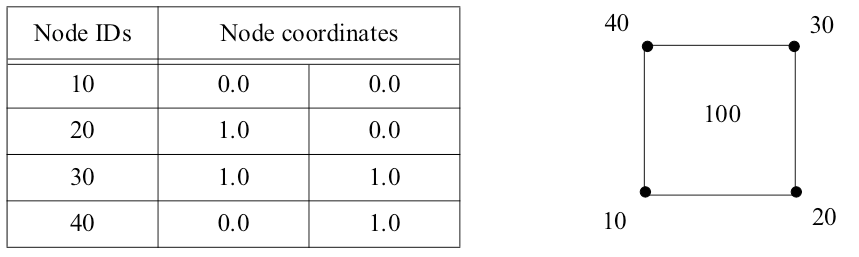
\includegraphics[width=5.972in, height=2.486in]{figures/UserDefinedNodeElementIds.png}
\caption{User-defined Node and Element IDs.}\label{f:UserDefinedNodeElementIds}
\end{center}
\end{figure}

The internal data structures representing the above model 
would be the following:


\begin{itemize}
 \item {nodal coordinate array}{:} {(0.0, 1.0, 1.0, 
0.0, 0.0, 0.0, 1.0, 1.0)}

 \item {connectivity array}{: (1, 2, 3, 4)}

 \item {node number map}{: (10, 20, 30, 40)}

 \item {element number map}{: (100)}
\end{itemize}


Internal (contiguously numbered) node and element IDs must be used for
all data structures that contain node or element numbers (IDs),
including node set node lists, side set element lists, and element
connectivity. Additionally, to inquire the value(s) of node or element
results variables, an application code must pass the internal node or
element number for the node or element of interest.




\section{Element Number Map}\label{s:enm}

\begin{spacing}{1.5}
\api \cfuncref{ex_put_elem_num_map}, \cfuncref{ex_get_elem_num_map}


\end{spacing}

{Refer to  Section 3.5 for a discussion of the optional element 
number map.}




\section{Optimized Element Order Map}\label{s:eom}

\begin{spacing}{1.5}
\api \cfuncref{ex_put_map}, \cfuncref{ex_get_map}


\end{spacing}

The optional element order map defines the element order in which a
solver (e.g., a wavefront solver) should process the elements. For
example, the first entry is the number of the element which should be
processed first by the solver. The length of this map is the total
number of elements in the model.

\section{Element Blocks}

For efficient storage and to minimize I/O, elements are grouped into
element blocks. Within an element block, all elements are of the same
type (basic geometry and number of nodes). This definition does not
preclude multiple element blocks containing the same element type
(i.e., ``QUAD'' elements may be in more than one element block); only
that each element block may contain only one element type.

The internal number of an element numbering is defined implicitly by
the order in which it appears in the file. Elements are numbered
internally (beginning with 1) consecutively across all element
blocks. See Section~\ref{s:enm} for a discussion of internal element
numbering.

\subsection{Element Block Parameters}\label{s:ebp}

\begin{spacing}{1.5}
\api \cfuncref{ex_put_elem_block}, \cfuncref{ex_get_elem_block}, \cfuncref{ex_get_elem_blk_ids}
\end{spacing}

The following parameters are defined for each element block:

\begin{itemize}
 \item element block ID -- an arbitrary, unique, positive integer
 which identifies the particular element block. This ID is used as a
 ``handle'' into the database that allows users to specify a group of
 elements to the application code without having to know the order in
 which element blocks are stored in the file.

 \item element type Element type -- a character string of length
 \param{MAX_STR_LENGTH} to distinguish element types. All elements
 within the element block are of this type. Refer to
 Table{\nobreakspace}1, ``Element Types and Attributes,'' on
 page{\nobreakspace}9 for a list of names that are currently
 accepted. It should be noted that the \exo{} library routines do not
 verify element type names against a standard list; the interpretation
 of the element type is left to the application codes which read or
 write the data. In general, the first three characters uniquely
 identify the element type. Application codes can append characters to
 the element type string (up to the maximum length allowed) to further
 classify the element for specific purposes.

 \item {Number of elements -- the number of elements in the 
element block.}

 \item {Nodes per element -- the number of nodes per element 
for the element block.}

 \item {Number of attributes -- the number of attributes per element
 in the element block. See below for a discussion of element
 attributes.}
\end{itemize}



\subsection{Element Connectivity}

\begin{spacing}{1.5}
\api \cfuncref{ex_put_elem_conn}, \cfuncref{ex_get_elem_conn}
\end{spacing}

The element connectivity contains the list of nodes (internal node
IDs; see Section~\ref{s:enm} for a discussion of node IDs) which
define each element in the element block. The length of this list is
the product of the number of elements and the number of nodes per
element as specified in the element block parameters. The node index
cycles faster than the element index. Node ordering follows the
conventions illustrated in Figure~\ref{f:NodeOrdering}, which includes ordering for
higher order elements. For lower order elements, simply omit the
unused nodes. These node ordering conventions follow the element
topology used in \code{PATRAN} [5]. Thus, for higher order elements than
those illustrated, use the ordering prescribed in the \code{PATRAN} User
Manual. For elements of type CIRCLE or SPHERE, the topology is one
node at the center of the circle or sphere element.
\begin{figure}[htbp]
\begin{center}
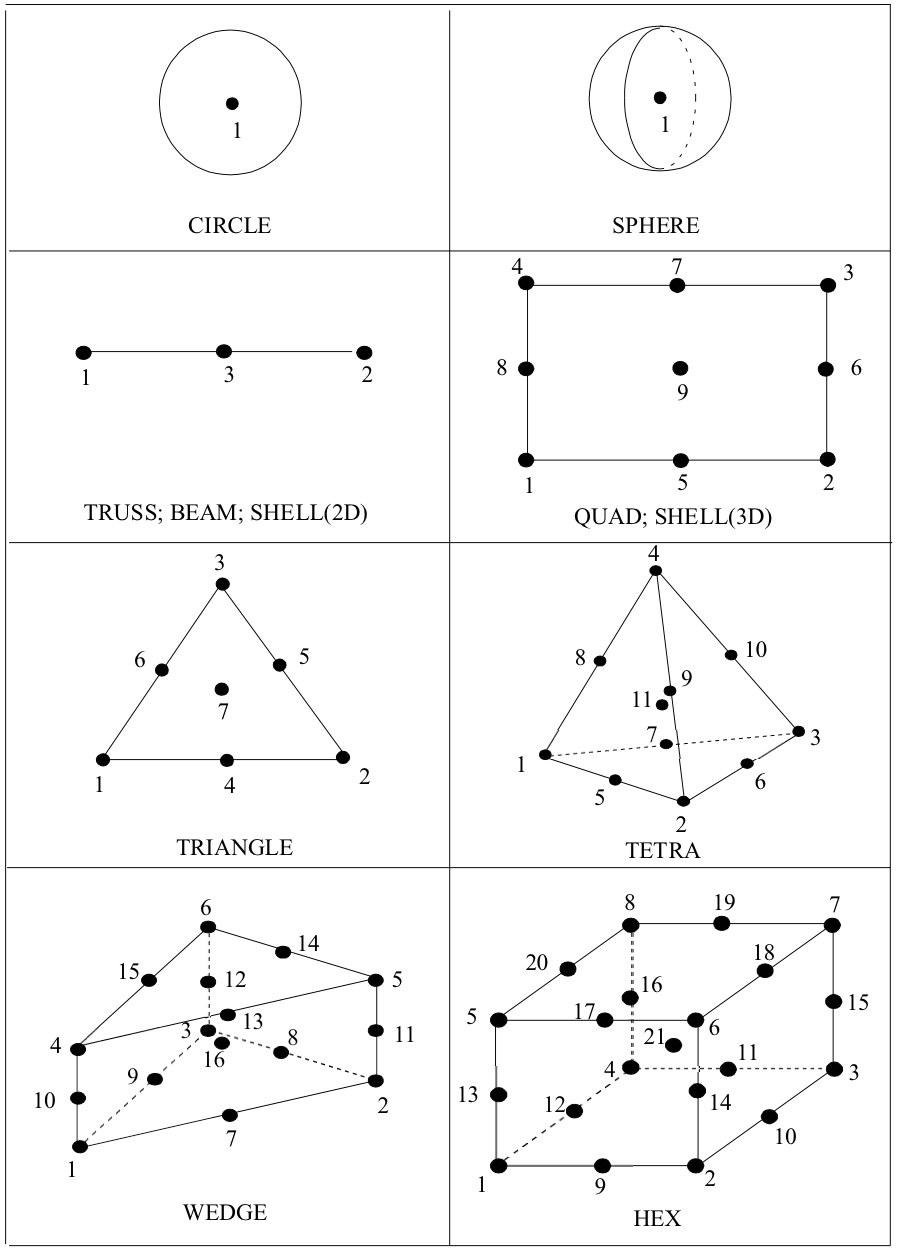
\includegraphics[width=6.250in, height=8.000in]{figures/NodeOrdering.png}
\caption{Node Ordering for Standard Element Types.}\label{f:NodeOrdering}
\end{center}
\end{figure}

\subsection{Element Attributes}

\begin{spacing}{1.5}
\api \cfuncref{ex_put_elem_attr}, \cfuncref{ex_get_elem_attr}
\end{spacing}

{Element attributes are optional floating point numbers that can be
assigned to each element. Every element in an element block must have
the same number of attributes (as specified in the element block
parameters) but the attributes may vary among elements within the
block. The length of the attributes array is thus the product of the
number of attributes per element and the number of elements in the
element block.  Table{\nobreakspace}1, ``Element Types and
Attributes,'' lists the standard attributes for the given element
types. }

\begin{table}[htbp]
\begin{center}
\begin{tabular}{|l|l|} \hline
Element Type & Attributes \\ \hline
CIRCLE   & R \\ \hline
SPHERE   & R \\ \hline
TRUSS    & A \\ \hline
BEAM     & 2D: A, I, J \\
         & 3D: A, $I_1$, $I_2$, J, $V_1$, $V_2$, $V_3$ \\ \hline
TRIANGLE & \\ \hline
QUAD     & \\ \hline
SHELL    & T \\ \hline
TETRA    & \\ \hline
PYRAMID  & \\ \hline
WEDGE    & \\ \hline
HEX      & \\ \hline
\end{tabular}
\end{center}
\end{table}

\section{Node Sets}

Node sets provide a means to reference a group of nodes with a single
ID. Node sets may be used to specify load or boundary
conditionsboundary conditions, or to identify nodes for a special
output request. A particular node may appear in any number of node
sets, but may be in a single node set only once. (This restriction is
not checked by \exo{} routines.) Node sets may be accessed
individually (using node set parameters, node set node list, and node
set distribution factors) or in a concatenated format (described in
Section 3.10 on page 11). The node sets data are stored identically in
the data file regardless of which method (individual or concatenated)
was used to output them.

\subsection{Node Set Parameters}

\begin{spacing}{1.5}
\api \cfuncref{ex_put_node_set_param}, \cfuncref{ex_get_node_set_param}, \cfuncref{ex_get_node_set_ids}
\end{spacing}

{The following parameters define each node set:}

\begin{itemize}
 \item {node set ID -- a unique positive integer that identifies the
 node set.}

 \item {Number of nodes -- the number of nodes in the node 
set.}

 \item {Number of node set distribution factors -- this should be zero
 if there are no distribution factors for the node set. If there are
 any distribution factors, this number must equal the number of nodes
 in the node set since the factors are assigned at each node. Refer to
 the discussion of distribution factors below.}
\end{itemize}



\subsection{Node Set Node List}

\begin{spacing}{1.5}
\api \cfuncref{ex_put_node_set}, \cfuncref{ex_get_node_set}
\end{spacing}

{This is an integer list of all the nodes in the node set. Internal
node IDs (see Section~\ref{s:enm}) must be used in this list.}



\subsection{Node Set Distribution Factors}

\begin{spacing}{1.5}
\api \cfuncref{ex_put_node_set_dist_fact}, \cfuncref{ex_get_node_set_dist_fact}
\end{spacing}

{This is an optional list of floating point factors associated with
the nodes in a node set. These data may be used as multipliers on
applied loads. If distribution factors are stored, each entry in this
list is associated with the corresponding entry in the node set node
list.}


\section{Concatenated Node Sets}

\begin{spacing}{1.5}
\api \cfuncref{ex_put_concat_node_sets}, \cfuncref{ex_get_concat_node_sets}
\end{spacing}

Concatenated node sets provide a means of writing/reading all node
sets with one function call. This is more efficient because it avoids
some I/O overhead, particularly when considering the intricacies of
the \code{NetCDF} library. (Refer to Appendix A for a discussion of
efficiency concerns.) This is accomplished with the following lists:

\begin{itemize}

 \item Node sets IDs -- list (of length number of node sets) 
of unique integer node set ID's. The \textit{{i}}\th{} entry in 
this list specifies the ID of the \textit{{i}}\th{} node set.

 \item Node sets node counts -- list (of length number of 
node sets) of counts of nodes for each node set. Thus, the \textit{{i}}\th{} 
entry in this list specifies the number of nodes in the \textit{{i}}\th{} 
node set.

 \item Node sets distribution factors counts -- list (of 
length number of node sets) of counts of distribution factors 
for each node set. The \textit{{i}}\th{} entry in this list specifies 
the number of distribution factors in the \textit{{i}}\th{} node 
set.

 \item Node sets node pointers -- list (of length number 
of node sets) of indices which are pointers into the node sets 
node list locating the first node of each node set. The \textit{{i}}\th{} 
entry in this list is an index in the node sets node list where 
the first node of the \textit{{i}}\th{} node set can be located.

 \item Node sets distribution factors pointers -- list (of 
length number of node sets) of indices which are pointers into 
the node sets distribution factors list locating the first factor 
of each node set. The \textit{{i}}\th{} entry in this list is an 
index in the node sets distribution factors list where the first 
factor of the \textit{{i}}\th{} node set can be located.

 \item Node sets node list -- concatenated integer list of the nodes
 in all the node sets. Internal node IDs (see Section~\ref{s:enm})
 must be used in this list. The node sets node pointers and node sets
 node counts are used to find the first node and the number of nodes
 in a particular node set.

 \item Node sets distribution factors list -- concatenated 
list of the (floating point) distribution factors in all the 
node sets. The node sets distribution factors pointers and node 
sets distribution factors counts are used to find the first factor 
and the number of factors in a particular node set.

\end{itemize}

To clarify the use of these lists, refer to the coding examples 
in  Section 4.2.25 and  Section 4.2.26.

\section{Side Sets}

Side sets provide a second means of applying load and boundary
conditions to a model. Unlike node sets, side sets are related to
specified sides of elements rather than simply a list of nodes. For
example, a pressure load must be associated with an element edge (in
2-d) or face (in 3-d) in order to apply it properly. Each side in a
side set is defined by an element number and a local edge (for 2-d
elements) or face (for 3-d elements) number. The local number of the
edge or face of interest must conform to the conventions as
illustrated in Figure~\ref{f:SideSetNumbering}.
\begin{figure}[htbp]
\begin{center}
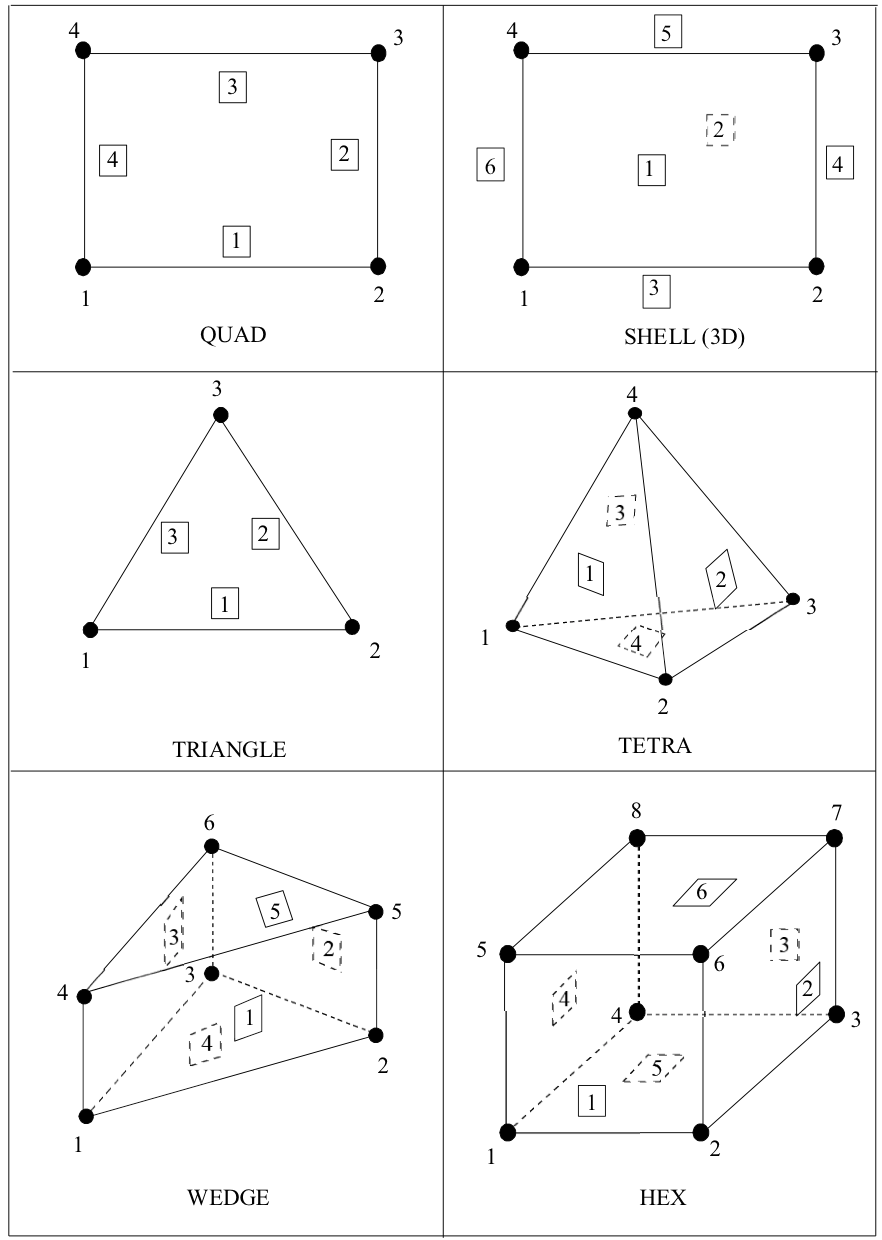
\includegraphics[width=6.250in, height=8.000in]{figures/SideSetNumbering.png}
\caption{Side Set Side Numbering.}\label{f:SideSetNumbering}
\end{center}
\end{figure}

 In this figure, side set side numbers are enclosed in boxes; only the
 essential node numbers to describe the element topology are shown. A
 side set may contain sides of differing types of elements that are
 contained in different element blocks. For instance, a single side
 set may contain faces of WEDGE elements, HEX elements, and TETRA
 elements.



\subsection{Side Set Parameters}



\begin{spacing}{1.5}
\api \cfuncref{ex_put_side_set_param}, \cfuncref{ex_get_side_set_param}, \cfuncref{ex_get_side_set_ids}
\end{spacing}

{The following parameters define each side set:}

\begin{itemize}
 \item {side set ID -- a unique positive integer that identifies the
 side set.}

 \item {Number of sides -- the number of sides in the side 
set.}

 \item {Number of side set distribution factors -- this should be zero
 if there are no distribution factors for the side set. If there are
 any distribution factors, they are assigned at the nodes on the sides
 of the side set. Refer to the discussion of distribution factors
 below.}
\end{itemize}

\subsection{Side Set Element List}



\begin{spacing}{1.5}
\api \cfuncref{ex_put_side_set}, \cfuncref{ex_get_side_set}
\end{spacing}

{This is an integer list of all the elements in the side set. 
Internal element IDs (see  Section~\ref{s:enm}) must be used 
in this list.}



\subsection{Side Set Side List}



\begin{spacing}{1.5}
\api \cfuncref{ex_put_side_set}, \cfuncref{ex_get_side_set}
\end{spacing}

{This is an integer list of all the sides in the side set. 
This list contains the local edge (for 2-d elements) or face 
(for 3-d elements) numbers following the conventions specified 
in  Figure 5.}



\subsection{Side Set Node List}



\begin{spacing}{1.5}
\api \cfuncref{ex_get_side_set_node_list}
\end{spacing}

It is important to note that the nodes on a side set are 
not explicitly stored in the data file, but can be extracted 
from the element numbers in the side set element list, local 
side numbers in the side set side list, and the element connectivity 
array. The node IDs that are output are internal node numbers 
(see  Section~\ref{s:nnm}). They are extracted according to 
the following conventions:


\begin{enumerate}
\item {All nodes for the first side (defined by the first element 
in the side set element list and the first side in the side set side
list) are output before the nodes for the second side. There is no
attempt to consolidate nodes; if a node is attached to four different
faces, then the same node number will be output four times -- once
each time the node is encountered when progressing along the side
list.}

\item {The nodes for a single face (or edge) are ordered to assist 
an application code in determining an ``outward'' direction. Thus, the
node list for a face of a 3-d element proceeds around the face so that
the outward normal follows the right-hand rule. The node list for an
edge of a 2-d element proceeds such that if the right hand is placed
in the plane of the element palm down, thumb extended with the index
(and other fingers) pointing from one node to the next in the list,
the thumb points to the inside of the element. This node ordering is
detailed in Table{\nobreakspace}2, ``Side Set Node Ordering,'' on
page{\nobreakspace}16.}

\item {The nodes required for a first-order element are output 
first, followed by the nodes of a higher ordered element. Again, this
is illustrated in Table{\nobreakspace}2, ``Side Set Node Ordering,'' }
\end{enumerate}

\begin{table}
\begin{center}
% use packages: array
\begin{tabular}{l|c|lll}
\hline \textbf{Element Type} & \textbf{Side \#}& \textbf{Node Order} \\ \hline
QUAD   & 1 & 1, 2, & 5 \\ 
(2D)   & 2 & 2, 3, & 6 \\ 
       & 3 & 3, 4, & 7 \\ 
       & 4 & 4, 1, & 8 \\ \hline
SHELL  & 1 & 1, 2, 3, 4, & 5, 6, 7, 8, & 9 \\ 
       & 2 & 1, 4, 3, 2, & 8, 7, 6, 5, & 9 \\ 
(Edges)& 3 & 1, 2, & 5 \\ 
       & 4 & 2, 3, & 6 \\ 
       & 5 & 3, 4, & 7 \\ 
       & 6 & 4, 1, & 8 \\ \hline
TRIANGLE&1 & 1, 2, & 4 \\ 
(2D)   & 2 & 2, 3, & 5 \\ 
       & 3 & 3, 1, & 6 \\ \hline
TRIANGLE& 1 & 1, 2, 3, & 4, 5, 6 \\ 
(Shell)& 2 & 1, 3, 2, & 6, 5, 4 \\ 
       & 3 & 1, 2,    & 4  \\
       & 4 & 2, 3,    & 5 \\
       & 5 & 3, 1,    & 6 \\ \hline
TETRA  & 1 & 1, 2, 4, & 5, 9, 8 \\ 
       & 2 & 2, 3, 4, & 6, 10, 9 \\ 
       & 3 & 1, 4, 3, & 8, 10, 7 \\ 
       & 4 & 1, 3, 2, & 7, 6, 5 \\ \hline
WEDGE  & 1 & 1, 2, 5, 4, & 7, 11, 13, 10 \\ 
       & 2 & 2, 3, 6, 5, & 8, 12, 14, 11 \\ 
       & 3 & 1, 4, 6, 3, & 10, 15, 12, 9 \\ 
       & 4 & 1, 3, 2, & 9, 8, 7 \\ 
       & 5 & 4, 5, 6, & 13, 14, 15 \\ \hline
HEX    & 1 & 1, 2, 6, 5, & 9, 14, 17, 13, & 26 \\ 
       & 2 & 2, 3, 7, 6, & 10, 15, 18, 14, & 25 \\ 
       & 3 & 3, 4, 8, 7, & 11, 16, 19, 15, & 27 \\ 
       & 4 & 1, 5, 8, 4, & 13, 20, 16, 12, & 24 \\ 
       & 5 & 1, 4, 3, 2, & 12, 11, 10, 9, & 22 \\ 
       & 6 & 5, 6, 7, 8, & 17, 18, 19, 20, & 23 \\ \hline
PYRAMID&1 & 1, 2, 5, & 6, 11, 10 \\ 
       & 2 & 2, 3, 5, & 7, 12, 11 \\ 
       & 3 & 3, 4, 5, & 8, 13, 12 \\ 
       & 4 & 4, 1, 5, & 9, 10, 13 \\ 
       & 5 & 1, 4, 3, 2, & 9, 8, 7, 6
\end{tabular}
\end{center}
\end{table}

\subsection{Side Set Node Count List}


\begin{spacing}{1.5}
\api \cfuncref{ex_get_side_set_node_list}
\end{spacing}

The length of the side set node count list is the length of the side
set element list. For each entry in the side set element list, there
is an entry in the side set side list, designating a local side
number. The corresponding entry in the side set node count list is the
number of nodes which define the particular side. In conjunction with
the side set node list, this node count array provides an unambiguous
nodal description of the side set.

\subsection{Side Set Distribution Factors}


\begin{spacing}{1.5}
\api \cfuncref{ex_put_side_set_dist_fact}, \cfuncref{ex_get_side_set_dist_fact}
\end{spacing}

This is an optional list of floating point factors associated with the
nodes on a side set. These data may be used for uneven application of
load or boundary conditions. Because distribution factors are assigned
at the nodes, application codes that utilize these factors must read
the side set node list. The distribution factors must be
stored/accessed in the same order as the nodes in the side set node
list; thus, the ordering conventions described above apply.


\section{Concatenated Side Sets}

\begin{spacing}{1.5}
\api \cfuncref{ex_put_concat_side_sets}, \cfuncref{ex_get_concat_side_sets}
\end{spacing}

Concatenated side sets provide a means of writing / reading all side
sets with one function call. This is more efficient because it avoids
some I/O overhead, particularly when considering the intricacies of
the \code{NetCDF} library. This is accomplished with the following
lists:
\begin{itemize}
 \item {Side sets IDs -- list (of length number of side sets) of
 unique positive integer side set ID's. The} \textit{{i}}{th entry in
 this list specifies the ID of the} \textit{{i}}{th side set.}

 \item {Side sets side counts -- list (of length number of side sets)
 of counts of sides for each side set. Thus, the} \textit{{i}}{th
 entry in this list specifies the number of sides in the}
 \textit{{i}}{th node set. This also defines the number of elements in
 each side set.}

 \item {Side sets distribution factors counts -- list (of length
 number of side sets) of counts of distribution factors for each side
 set. The} \textit{{i}}{th entry in this list specifies the number of
 distribution factors in the} \textit{{i}}{th side set.}

 \item {Side sets side pointers -- list (of length number of side
 sets) of indices which are pointers into the side sets element list
 (and side list) locating the first element (or side) of each side
 set. The} \textit{{i}}{th entry in this list is an index in the side
 sets element list (and side list) where the first element (or side)
 of the} \textit{{i}}{th side set can be located.}

 \item {Side sets distribution factors pointers -- list (of length
 number of side sets) of indices which are pointers into the side sets
 distribution factors list locating the first factor of each side
 set. The} \textit{{i}}{th entry in this list is an index in the side
 sets distribution factors list where the first factor of the}
 \textit{{i}}{th side set can be located.}

 \item {Side sets element list -- concatenated integer list of the
 elements in all the side sets.} {Internal element IDs (see
 Section~\ref{s:enm}) must be used in this list.} {The side sets side
 pointers and side sets side counts are used to find the first element
 and the number of elements in a particular side set.}

 \item {Side sets side list -- concatenated integer list of the sides
 in all the side sets. The side sets side pointers and side sets side
 counts are used to find the first side and the number of sides in a
 particular side set.}

 \item {Side sets distribution factors list -- concatenated list of
 the (floating point) distribution factors in all the side sets. The
 side sets distribution factors pointers and side sets distribution
 factors counts are used to find the first factor and the number of
 factors in a particular side set.}
\end{itemize}



\subsection{Object Properties}

Certain \exo{} objects (currently element blocks, node 
sets, and side sets) can be given integer properties, providing 
the following capabilitities:
\begin{enumerate}
\item assign a specific integer value to a named property of 
an object.

\item tag objects as members of a group. For example element 
blocks 1 and 3 and side sets 1 and 2 could be put in a group 
named ``TOP.''
\end{enumerate}

This functionality is illustrated in Table{\nobreakspace}3, ``Sample
Property Table,'' which contains the property values of a sample
\exo{} file with three element blocks, one node set, and two 
side sets. Note that an application code can define properties 
to be valid for only specified object types. In this example, 
``STEEL'' and ``COPPER'' are valid for all element blocks but are 
not defined for node sets and side sets. 

\begin{figure}[htbp]
\begin{center}
%\includegraphics[width=6.250in, height=2.722in]{exodusIIFig8.wmf}
\caption{exodusIIFig8.wmf about here.}
\end{center}
\end{figure}


{Interpretation of the integer values of the properties is left to the
application codes, but in general, a nonzero positive value means the
object has the named property (or is in the named group); a zero means
the object does not have the named property (or is not in the named
group). Thus, element block 1 has an ID of 10 (1 is a counter internal
to the data base; an application code accesses the element block using
the ID), node set 1 has an ID of 100, etc. The group ``TOP'' includes
element block 1, element block 3, and side sets 1 and 2.}



\subsection{Property Values}



\begin{spacing}{1.5}
\api \cfuncref{ex_put_prop}, \cfuncref{ex_get_prop}, \cfuncref{ex_put_prop_array}, \cfuncref{ex_get_prop_array}
\end{spacing}

Valid values for the properties are positive integers and
zero. Property values are stored in arrays in the data file but can be
written / read individually given an object type (i.e., element block,
node set, or side set), object ID, and property name or as an array
given an object type and property name. If accessed as an array, the
order of the values in the array must correspond to the order in which
the element blocks, node sets, or side sets were introduced into the
file. For instance, if the parameters for element block with ID 20
were written to a file, and then parameters for element block with ID
10, followed by the parameters for element block with ID 30, the
first, second, and third elements in the property array would
correspond to element block 20, element block 10, and element block
30, respectively. This order can be determined with a call to
\cfuncref{ex_get_elem_blk_ids} which returns an array of element
block IDs in the order that the corresponding element blocks were
introduced to the data file.

\section{Results Parameters}

\api\cfuncref{ex_put_variable_param}, \cfuncref{ex_get_variable_param}


The number of each type of results variables (element, nodal, 
and global) is specified only once, and cannot change through 
time.

\subsection{Results Names}

\begin{spacing}{1.5}
\api \cfuncref{ex_put_variable_names}, \cfuncref{ex_get_variable_names}
\end{spacing}

Associated with each results variable is a unique name of 
length \param{MAX_STR_LENGTH}.



\section{Results Data}


An integer output time step number (beginning with 1) is used as an
index into the results variables written to or read from an \exo{}
file. It is a counter of the number of ``data planes'' that have been
written to the file. The maximum time step number (i.e., the number of
time steps that have been written) is available via a call to the
database inquire function ( See Section~\ref{s:inquire}). For each
output time step, the following information is stored.

\subsection{Time Values}

\begin{spacing}{1.5}
\api \cfuncref{ex_put_time}, \cfuncref{ex_get_time}, \cfuncref{ex_get_all_times}
\end{spacing}

A floating point value must be stored for each time step to identify
the ``data plane.'' Typically, this is the analysis time but can be
any floating point variable that distinguishes the time steps. For
instance, for a modal analysis, the natural frequency for each mode
may be stored as a ``time value'' to discriminate the different sets
of eigen vectors. The only restriction on the time values is that they
must monotonically increase.

\subsection{Global Results}

\begin{spacing}{1.5}
\api \cfuncref{ex_put_glob_vars}, \cfuncref{ex_get_glob_vars}, \cfuncref{ex_get_glob_var_time}
\end{spacing}

This object contains the floating point global data for the time
step. The length of the array is the number of global variables, as
specified in the results parameters.


\subsection{Nodal Results}

\begin{spacing}{1.5}
\api \cfuncref{ex_put_nodal_var}, \cfuncref{ex_get_nodal_var}, \cfuncref{ex_get_nodal_var_time}
\end{spacing}

This object contains the floating point nodal data for the 
time step. The size of the array is the number of nodes, as specified 
in the global parameters, times the number of nodal variables.

\subsection{Element Results}

\begin{spacing}{1.5}
\api \cfuncref{ex_put_elem_var}, \cfuncref{ex_get_elem_var}, \cfuncref{ex_get_elem_var_time}
\end{spacing}

Element variables are output for a given element block and a given
element variable. Thus, at each time step, up to \textit{{m}} element
variable objects (where \textit{{m}} is the product of the number of
element blocks and the number of element variables) may be
stored. However, since not all element variables must be output for
all element blocks (see the next section), \textit{{m}} is the
\textit{{maximum}} number of element variable objects. The actual
number of objects stored is the number of unique combinations of
element variable index and element block ID passed to
\cfuncref{ex_put_elem_var} or the number of non-zero entries in the
element variable truth table (if it is used). The length of each
object is the number of elements in the given element block.


\section{Element Variable Truth Table}


\begin{spacing}{1.5}
\api \cfuncref{ex_put_elem_var_tab}, \cfuncref{ex_get_elem_var_tab}
\end{spacing}

Because some element variables are not applicable (and thus not
computed by a simulation code) for all element types, the element
variable truth table is an optional mechanism for specifying whether a
particular element result is output for the elements in a particular
element block. For example, hydrostatic stress may be an output result
for the elements in element block 3, but not those in element block 6.


It is helpful to describe the element variable truth 
table as a two-dimensional array, as shown in  Table{\nobreakspace}4, 
``Element Variable Truth Table,'' Each row of the array is associated 
with an element variable; each column of the array is associated 
with an element block. If a datum in the truth table is zero 
$(\textrm{table}(i,j)=0)$, then no results are output for the {i}\th{} 
element variable for the {j}\th{} element block. A nonzero 
entry indicates that the appropriate result will be output. In 
this example, element variable 1 will be stored for all element 
blocks; element variable 2 will be stored for element blocks 
1 and 4; and element variable 3 will be stored for element blocks 
3 and 4. The table is stored such that the variable index cycles 
faster than the block index.
\begin{figure}[htbp]
\begin{center}
%\includegraphics[width=6.250in, height=1.708in]{exodusIIFig9.wmf}
\caption{exodusIIFig9.wmf about here.}
\end{center}
\end{figure}

\chapter{Application Programming Interface (API)}


\exo{} files can be written and read by application codes 
written in C, C++, or Fortran via calls to functions in the application 
programming interface (API). Functions within the API are categorized 
as data file utilities, model description functions, or results 
data functions. 

In general, the following pattern is followed for writing 
data objects to a file:

\begin{enumerate}
\item create the file with \cfuncref{ex_create};
\item write out global parameters to the file using \cfuncref{ex_put_init};
\item write out specific data object parameters; for example, 
put out element block parameters with \cfuncref{ex_put_elem_block};
\item write out the data object; for example, put out the connectivity 
for an element block with \cfuncref{ex_put_elem_conn};
\item close the file with \cfuncref{ex_close}.
\end{enumerate}

Steps 3 and 4 are repeated within this pattern for each data object
(i.e., nodal coordinates, element blocks, node sets, side sets,
results variables, etc.). For some data object types, steps 3 and 4
are combined in a single call. For instance, \cfuncref{ex_put_qa}
writes out the parameters (number of QA records) as well as the data
object itself (the QA records). During the database writing process,
there are a few order dependencies (e.g., an element block must be
written before element variables for that element block are written)
which are documented in the description of each library function.


The invocation of the \exo{} API functions for reading 
data is order independent, providing random read access. The 
following steps are typically used for reading data:

\begin{enumerate}

\item open the file with \cfuncref{ex_open};

\item read the global parameters for dimensioning purposes with
\cfuncref{ex_get_init};

\item read specific data object parameters; for example, read 
node set parameters with \cfuncref{ex_get_node_set_param};

\item read the data object; for example, read the node set node 
list with \cfuncref{ex_get_node_set};

\item close the file with \cfuncref{ex_close}.
\end{enumerate}

Again, steps 3 and 4 are repeated for each object. For some object
parameters, step 3 may be accomplished with a call to \cfuncref{ex_inquire}
 to inquire the size of certain objects.


In developing applications using the \exo{} API, the following
points may prove beneficial:

\begin{itemize}

 \item All functions that write objects to the database begin with
 \cfuncref{ex_put_}; functions that read objects from
 the database begin with \cfuncref{ex_get_}.

 \item Function arguments are classified as readable \R{}, writable
 \W{}, or both \RW{}. Readable arguments are not modified by the API
 routines; writable arguments are modified; read-write arguments may
 be either depending on the value of the argument.

 \item All application codes which use the \exo{} API must include
 the file `exodusII.h' for C. This file defines constants that are
 used (1) as arguments to the API routines, (2) to set global
 parameters such as maximum string length and database version, and
 (3) as error condition or function return values.

 \item Throughout this section, sample code segments have been
 included to aid the application developer in using the API
 routines. These segments are not complete and there has been no
 attempt to include all calling sequence dependencies within
 them.

 \item Because 2-dimensional arrays cannot be statically dimensioned,
 either dynamic dimensioning or user indexing is required. Most of the
 sample code segments utilize user indexing within 1-dimensional
 arrays even though the variables are logically 2-dimensional.

 \item There are many \code{NetCDF} utilities that prove useful. ncdump,
 which converts a binary \code{NetCDF} file to a readable ASCII version of
 the file, is the most notable.

 \item Because \code{NetCDF} buffers I/O, it is important to flush
 all buffers with \cfuncref{ex_update} when debugging an
 application that produces an \exo{} file.
\end{itemize}

\section{Data File Utilities}\label{sec:utilities}

This section describes data file utility functions for creating /
opening a file, initializing a file with global parameters, reading /
writing information text, inquiring on parameters stored in the data
file, and error reporting.

\subsection{Create \exo{} File}

The function \cfuncref{ex_create} creates a new
\exo{} file and returns an ID that can subsequently be used to
refer to the file.

All floating point values in an \exo{} file are stored as either
4-byte (``float'') or 8-byte (``double'') numbers; no mixing
of 4- and 8-byte numbers in a single file is allowed. An application
code can compute either 4- or 8-byte values and can designate that the
values be stored in the \exo{} file as either 4- or 8-byte numbers;
conversion between the 4- and 8-byte values is performed automatically
by the API routines. Thus, there are four possible combinations of
compute word size and storage (or I/O) word size.

In case of an error, \cfuncref{ex_create} returns a negative
number. Possible causes of errors include:

\begin{itemize}

 \item Passing a file name that includes a directory that does not
 exist.

 \item Specifying a file name of a file that exists and also
 specifying a no clobber option.

 \item Attempting to create a file in a directory without permission
 to create files there.

 \item Passing an invalid file clobber mode.
\end{itemize}

\funcdef{ex_create}{char~*path, int~mode, int~*comp_ws, int~*io_ws}

\begin{parameters}
\item[{char* path \R{}}]
The file name of the new \exo{} file. This can be given as either an
absolute path name (from the root of the file system) or a relative
path name (from the current directory).


\item[{int mode \R{}}]
Mode. Use one of the following predefined constants:

\begin{description}
\item[\param{EX_NOCLOBBER}] 
To create the new file only if the given file name does not refer to a
file that already exists.

\item[\param{EX_CLOBBER}] 
To create the new file, regardless of whether a file with the same
name already exists. If a file with the same name does exist, its
contents will be erased.

\item[\param{EX_LARGE_MODEL}] 
To create a model that can store individual datasets larger than
2~gigabytes. This modifies the internal storage used by exodusII and
also puts the underlying \code{NetCDF} file into the ``64-bit offset''
mode. See Appendix~\ref{app:largemodel} for more details on this
mode.\footnote{A ``large model'' file will also be created if the
environment variable
\code{EXODUS_LARGE_MODEL}\index{Environment
Variable!EXODUS_LARGE_MODEL}\index{EXODUS_LARGE_MODEL} is defined
in the users environment. A message will be printed to standard output
if this environment variable is found.}

\item[\param{EX_NORMAL_MODEL}] 
Create a standard model.

\item[\param{EX_NETCDF4}] 
To create a model using the \code{HDF5}-based \code{NetCDF-4}
output. (Future capability)\footnote{\code{NetCDF-4} is currently in
beta mode; however, it will be used for ExodusII when available, so
this mode is being defined here for future completeness. An
\code{HDF5}-based \code{NetCDF-4} file will also be created if the
environment variable \code{EXODUS_NETCDF4}\index{Environment
Variable!EXODUS_NETCDF4}\index{EXODUS_NETCDF4} is defined in the
users environment. A message will be printed to standard output if
this environment variable is found.}

\item[\param{EX_NOSHARE}] 
Do not open the underlying \code{NetCDF} file in ``share'' mode. See the
\code{NetCDF} documentation for more details.

\item[\param{EX_SHARE}] 
Do open the underlying \code{NetCDF} file in ``share'' mode. See the \code{NetCDF}
documentation for more details.
\end{description}

\item[{int* comp_ws \RW{}}] 
{The word size in bytes (0, 4 or 8) of the floating point variables
used in the application program. If 0 (zero) is passed, the default
sizeof(float) will be used and returned in this variable. WARNING: all
\exo{} functions requiring floats must be passed floats declared with
this passed in or returned compute word size (4 or 8).}

\item[{int* io_ws \R{}}] {The word size in bytes (4 or 8) of the 
floating point data as they are to be stored in the \exo{} file.}
\end{parameters}

The following code segment creates an \exo{} file called \file{test.exo}:

\begin{lstlisting}
#include "exodusII.h"
int CPU_word_size, IO_word_size, exoid;
CPU_word_size = sizeof(float); /* use float or double */
IO_word_size = 8; /* store variables as doubles */

/* create \exo{} file */
exoid = ex_create ("test.exo"      /* filename path */
		    EX_CLOBBER,     /* create mode */
		    &CPU_word_size, /* CPU float word size in bytes */
	            &IO_word_size); /* I/O float word size in bytes */
\end{lstlisting}


\subsection{Open \exo{} File}

The function \cfuncref{ex_open} opens an existing \exo{} file and
returns an ID that can subsequently be used to refer to the file, the
word size of the floating point values stored in the file, and the
version of the \exo{} database (returned as a ``float'', regardless of
the compute or I/O word size). Multiple files may be ``open''
simultaneously.


In case of an error, \cfuncref{ex_open} returns a negative
number. Possible causes of errors include:

\begin{itemize}
\item The specified file does not exist.

 \item The mode specified is something other than the predefined 
constant \param{EX_READ} or \param{EX_WRITE}.


 \item Database version is earlier than 2.0.
\end{itemize}


\funcdef{ex_open}{char~*path, int~mode, int~*comp_ws, int~*io_ws, float~*version}

\begin{parameters}
\item[{char* path \R{}}]
The file name of the \exo{} file. This can be given as either an
absolute path name (from the root of the file system) or a relative
path name (from the current directory).

\item[{int mode \R{}}]
Access mode. Use one of the following predefined constants:

\begin{description}
 \item [EX_READ] To open the file just for reading.

 \item [EX_WRITE] To open the file for writing and reading.
\end{description}

\item[{int* comp_ws \RW{}}]
The word size in bytes (0, 4 or 8) of the floating point variables
used in the application program. If 0 (zero) is passed, the default
size of floating point values for the machine will be used and
returned in this variable. WARNING: all \exo{} functions requiring
reals must be passed reals declared with this passed in or returned
compute word size (4 or 8).


\item[{int* io_ws \RW{}}]
The word size in bytes (0, 4 or 8) of the floating 
point data as they are stored in the \exo{} file. If the word 
size does not match the word size of data stored in the file, 
a fatal error is returned. If this argument is 0, the word size 
of the floating point data already stored in the file is returned.

\item[{float* version \W{}}]
Returned \exo{} database version number. The current version is
\version{}
\end{parameters}

The following opens an \exo{} file named \file{test.exo} for read
only, using default settings for compute and I/O word sizes:

\begin{lstlisting}
#include "exodusII.h"
int CPU_word_size,IO_word_size, exoid;
float version;

CPU_word_size = sizeof(float);   /* float or double */
IO_word_size = 0;                /* use what is stored in file */

/* open \exo{} files */
exoid = ex_open ("test.exo",     /* filename path */
	         EX_READ,        /* access mode = READ */
		 &CPU_word_size, /* CPU word size */
		 &IO_word_size,  /* IO word size */
	         &version);      /* ExodusII library version */
\end{lstlisting}


\subsection{Close \exo{} File}

The function \cfuncref{ex_close} updates and
then closes an open \exo{} file.

In case of an error, \cfuncref{ex_close} returns a negative number; a
warning will return a positive number. Possible causes of errors
include:
\begin{itemize}
 \item data file not properly opened with call to \cfuncref{ex_create} or
 \cfuncref{ex_open}
\end{itemize}


\funcdef{ex_close}{int~exoid}

\begin{parameters}
\item[{int exoid \R{}}]
\exo{} file ID returned from a previous call to \cfuncref{ex_create} 
or \cfuncref{ex_open}.
\end{parameters}

The following code segment closes an open \exo{} file:

\begin{lstlisting}
int error,exoid;
error = ex_close (exoid);
\end{lstlisting}



\subsection{Write Initialization Parameters}

The function \cfuncref{ex_put_init} writes the
initialization parameters to the \exo{}
file. This function must be called once (and only once) before
writing any data to the file.


In case of an error, \cfuncref{ex_put_init} returns a negative number;
a warning will return a positive number.  Possible causes of errors
include:

\begin{itemize}
 \item data file not properly opened with call to \cfuncref{ex_create} or
 \cfuncref{ex_open}

 \item data file opened for read only.

 \item this routine has been called previously.
\end{itemize}


\funcdef{ex_put_init}{int~exoid, char~*title, int~num_dim, int~num_nodes, 
int~num_elem, int~num_elem_blk, int~num_node_sets, int~num_side_sets}

\begin{parameters}
\item[int exoid \R{}]
\exo{} file ID returned from a previous call to \cfuncref{ex_create} 
or \cfuncref{ex_open}.

\item[{char* titletitle \R{}}]
Database title. Maximum length is \param{MAX_LINE_LENGTH}.

\item[{int num_dim \R{}}]
The dimensionality of the database. This is the number of coordinates
per node.

\item[{int num_nodes \R{}}] 
The number of nodal points.

\item[{int num_elem \R{}}]
The number of elements.

\item[{int num_elem_blk \R{}}]
The number of element blocks.

\item[{int num_node_sets \R{}}]
The number of node sets.

\item[{int num_side_sets \R{}}]
The number of side sets.
\end{parameters}

The following code segment will initialize an open \exo{} file with
the specified parameters:

\begin{lstlisting}
int num_dim, num_nods, num_el, num_el_blk, num_ns, num_ss, error, exoid;

/* initialize file with parameters */
num_dim = 3; num_nods = 46; num_el = 5; num_el_blk = 5;
num_ns = 2; num_ss = 5;

error = ex_put_init (exoid, "This is the title", num_dim, 
                     num_nods, num_el,num_el_blk, num_ns, num_ss);
\end{lstlisting}


\subsection{Read Initialization Parameters}

The function \cfuncref{ex_get_init} reads the
initializationinitialization parameters from an opened
\exo{} file.

In case of an error, \cfuncref{ex_get_init} returns a negative number;
a warning will return a positive number. Possible causes of errors
include:

\begin{itemize}
 \item data file not properly opened with call to \cfuncref{ex_create} 
or \cfuncref{ex_open}.
\end{itemize}

\funcdef{ex_get_init}{int~exoid, char~*title, int~num_dim, int~num_nodes, 
int~num_elem, int~num_elem_blk, int~num_node_sets, int~num_side_sets}

\begin{parameters}
\item[{int exoid \R{}}]
\exo{} file ID returned from a previous call to \cfuncref{ex_create} 
or \cfuncref{ex_open}.

\item[{char* titletitle \W{}}]
Returned database title. String length may be up to
\param{MAX_LINE_LENGTH} bytes.

\item[{int* num_dim \W{}}]
Returned dimensionality of the database. This is the number of
coordinates per node.

\item[{int* num_nodes \W{}}]
Returned number of nodal points.

\item[{int* num_elem \W{}}]
Returned number of elements.

\item[{int* num_elem_blk \W{}}]
Returned number of element blocks.

\item[{int* num_node_sets \W{}}]
Returned number of node sets.

\item[{int* num_side_sets \W{}}]
Returned number of side sets.
\end{parameters}

The following code segment will read the initialization parameters
from the open \exo{} file:

\begin{lstlisting}
#include "exodusII.h"
int num_dim, num_nodes, num_elem, num_elem_blk,
    num_node_sets, num_side_sets, error, exoid;

char title[MAX_LINE_LENGTH+1];

/* read database parameters */
error = ex_get_init (exoid, title, &num_dim, &num_nodes, 
                     &num_elem, &num_elem_blk, &num_node_sets, &num_side_sets);
\end{lstlisting}


\subsection{Write Quality Assurance (QA) Records}


The function \cfuncref{ex_put_qa} writes the QA records to the
database. Each QA record contains four \param{MAX_STR_LENGTH}-byte
character strings. The character strings are:

\begin{itemize}
\item the analysis code name
\item the analysis code QA descriptor
\item the analysis date
\item the analysis time
\end{itemize}

In case of an error, \cfuncref{ex_put_qa} returns a negative number; a
warning will return a positive number. Possible causes of errors
include:

\begin{itemize}
 \item data file not properly opened with call to \cfuncref{ex_create} or
 \cfuncref{ex_open}

 \item data file opened for read only.

 \item QA records already exist in file.
\end{itemize}


\funcdef{ex_put_qa}{int~exoid, int~num_qa_records, char~*qa_record[][4]}

\begin{parameters}
\item[{int exoid \R{}}]
\exo{} file ID returned from a previous call to \cfuncref{ex_create} or
\cfuncref{ex_open}.

\item[{int num_qa_records \R{}}]
The number of QA records.

\item[{char* qa_record \R{}}]
Array containing the QA records.
\end{parameters}

The following code segment will write out two QA records:

\begin{lstlisting}
#include "exodusII.h"
int num_qa_rec, error, exoid;
char *qa_record[2][4];

/* write QA records */
num_qa_rec = 2;

qa_record[0][0] = "TESTWT1";
qa_record[0][1] = "testwt1";
qa_record[0][2] = "07/07/93";
qa_record[0][3] = "15:41:33";
qa_record[1][0] = "FASTQ";
qa_record[1][1] = "fastq";
qa_record[1][2] = "07/07/93";
qa_record[1][3] = "16:41:33";

error = ex_put_qa (exoid, num_qa_rec, qa_record);
\end{lstlisting}




\subsection{Read Quality Assurance (QA) Records}

The function \cfuncref{ex_get_qa} reads the QA records from the
database. Each QA record contains four \param{MAX_STR_LENGTH}-byte
character strings. The character strings are:

\begin{itemize}
\item the analysis code name
\item the analysis code QA descriptor
\item the analysis date
\item the analysis time
\end{itemize}

Memory must be allocated for the QA records before this call is
made. The number of QA records can be determined by invoking
\cfuncref{ex_inquire}.

In case of an error, \cfuncref{ex_get_qa} returns a negative number; a
warning will return a positive number.  Possible causes of errors
include:

\begin{itemize}
 \item data file not properly opened with call to \cfuncref{ex_create} or
 \cfuncref{ex_open}

 \item a warning value is returned if no QA records were stored.
\end{itemize}

\funcdef{ex_get_qa}{int~exoid, char~*qa_record[][4]}

\begin{parameters}
\item[{int exoid \R{}}]
\exo{} file ID returned from a previous call to \cfuncref{ex_create} 
or \cfuncref{ex_open}.

\item[{char* qa_record \W{}}]
Returned array containing the QA records.
\end{parameters}


The following will determine the number of QA records and 
read them from the open \exo{} file:

\begin{lstlisting}
#include "exodusII.h"
int num_qa_rec, error, exoid
char *qa_record[MAX_QA_REC][4];

/* read QA records */
num_qa_rec = ex_inquire_int(exoid, EX_INQ_QA);

for (i=0; i\texttt{<}num_qa_rec; i++) {
    for (j=0; j\texttt{<}4; j++)
    qa_record[i][j] = (char *) calloc ((MAX_STR_LENGTH+1), sizeof(char));
}
error = ex_get_qa (exoid, qa_record);
\end{lstlisting}


\subsection{Write Information Records}

The function \cfuncref{ex_put_info} writes information records to the
database. The records are MAX_LINE_LENGTH-character strings.

In case of an error, \cfuncref{ex_put_info} returns a negative number;
a warning will return a positive number. Possible causes of errors
include:

\begin{itemize}

 \item data file not properly opened with call to \cfuncref{ex_create}
 or \cfuncref{ex_open}

 \item data file opened for read only.

 \item information records already exist in file.
\end{itemize}

\funcdef{ex_put_info}{int~exoid, int~num_info, char~**info}


\begin{parameters}
\item[{int exoid \R{}}]
\exo{} file ID returned from a previous call to \cfuncref{ex_create} or
\cfuncref{ex_open}.


\item[{int num_info \R{}}]
The number of information records.


\item[{char** info \R{}}]
Array containing the information records.
\end{parameters}

The following code will write out three information records 
to an open \exo{} file:

\begin{lstlisting}
#include "exodusII.h"
int error, exoid, num_info;
char *info[3];

/* write information records */
num_info = 3;

info[0] = "This is the first information record.";
info[1] = "This is the second information record.";
info[2] = "This is the third information record.";

error = ex_put_info(exoid, num_info, info);
\end{lstlisting}

\subsection{Read Information Records}

The function \cfuncref{ex_get_info} reads information records from the
database. The records are \param{MAX_LINE_LENGTH}-character
strings. Memory must be allocated for the information records before
this call is made. The number of records can be determined by invoking
\cfuncref{ex_inquire} or \cfuncref{ex_inquire_int}.


In case of an error, \cfuncref{ex_get_info} returns a negative number;
a warning will return a positive number. Possible causes of errors
include:


\begin{itemize}
 \item data file not properly opened with call to \cfuncref{ex_create} or
 \cfuncref{ex_open}

 \item a warning value is returned if no information records were
 stored.
\end{itemize}



\funcdef{ex_get_info}{int~exoid, char`**info}


\begin{parameters}
\item[{int exoid \R{}}]
\exo{} file ID returned from a previous call to \cfuncref{ex_create} 
or \cfuncref{ex_open}.

\item[char** info \W{}]
Returned array containing the information records.
\end{parameters}

The following code segment will determine the number of information 
records and read them from an open \exo{} file:


\begin{lstlisting}
#include "exodusII.h"
int error, exoid, num_info;
char *info[MAXINFO];

/* read information records */
num_info = ex_inquire_int (exoid,EX_INQ_INFO);
for (i=0; i < num_info; i++) {
   info[i] = (char *) calloc ((MAX_LINE_LENGTH+1), sizeof(char));
}
error = ex_get_info (exoid, info);
\end{lstlisting}



\subsection{Inquire \exo{} Parameters}\label{s:inquire}


The function \cfuncref{ex_inquire} is used to inquire values of certain
data entities in an \exo{} file. Memory must be allocated for the
returned values before this function is invoked.query database


In case of an error, \cfuncref{ex_inquire} returns a negative 
number; a warning will return a positive number.
Possible causes of errors include:

\begin{itemize}
 \item data file not properly opened with call to \cfuncref{ex_create} or
 \cfuncref{ex_open}.
 \item requested information not stored in the file.
 \item invalid request flag.
\end{itemize}


\funcdef{ex_inquire}{int~exoid, ex_inquiry~req_info, int~*ret_int, float~*ret_float, char~*ret_char}

\begin{parameters}
\item[{int exoid \R{}}]
\exo{} file ID returned from a previous call to \cfuncref{ex_create} 
or \cfuncref{ex_open}.

\item[{ex_inquiry req_info \R{}}]
A flag which designates what information is requested. It must be one
of the following constants (predefined in the file
\file{exodusII.h}):

\begin{longtable}{@{}lp{4.4in}}
 \param{EX_INQ_API_VERS}& The \exo{} API version number is returned
 in \cmd{ret_float} and an ``undotted'' version number is returned in
 \cmd{ret_int}. The API version number reflects the release of the
 function library (i.e., function names, argument list, etc.). The
 current API version is {\version} or {\versionud}\footnote{The API
 and DB version numbers are synchronized and will always
 match. Initially, it was thought that maintaining the two versions
 separately would be a benefit, but that was more confusing than
 helpful, so the numbers were made the same awhile ago}.\\

 \param{EX_INQ_DB_VERS}& The \exo{} database version number is
 returned in \cmd{ret_float} and an ``undotted'' version number is
 returned in \cmd{ret_int}. The database version number reflects the
 version of the library that was used to write the file pointed to by
 \cmd{exoid}. The current database version is {\version} or
 {\versionud}.\\

 \param{EX_INQ_LIB_VERS}& The \exo{} library version number is
 returned in \cmd{ret_float} and an ``undotted'' version number is
 returned in \cmd{ret_int}. The API library version number reflects
 the version number of the \exo{} library linked with this
 application. The current library version is {\version} or
 {\versionud}\\

 \param{EX_INQ_TITLE}& The title stored in the database is returned
 in \cmd{ret_char}.\\

 \param{EX_INQ_DIM}& The dimensionality, or number of coordinates
 per node (1, 2 or 3), of the database is returned in
 \cmd{ret_int}.\\

 \param{EX_INQ_NODES}& The number of nodes is returned in
 \cmd{ret_int}.\\

 \param{EX_INQ_ELEM}& The number of elements is returned in
 \cmd{ret_int}.\\

 \param{EX_INQ_ELEM_BLK}& The number of element blocks is returned
 in \cmd{ret_int}.\\

 \param{EX_INQ_NODE_SETS}& The number of node sets is returned in
 \cmd{ret_int}.\\

 \param{EX_INQ_NS_NODE_LEN}& The length of the concatenated node
 sets node list is returned in \cmd{ret_int}.\\

 \param{EX_INQ_NS_DF_LEN}& The length of the concatenated node
 sets distribution list is returned in \cmd{ret_int}.\\

 \param{EX_INQ_SIDE_SETS}& The number of side sets is returned in
 \cmd{ret_int}.\\

 \param{EX_INQ_SS_ELEM_LEN}& The length of the concatenated side
 sets element list is returned in \cmd{ret_int}.\\

 \param{EX_INQ_SS_DF_LEN}& The length of the concatenated side
 sets distribution factor list is returned in \cmd{ret_int}.\\

 \param{EX_INQ_SS_NODE_LEN}& The aggregate length of all of the
 side sets node lists is returned in \cmd{ret_int}.\\

 \param{EX_INQ_EB_PROP}& The number of integer properties stored
 for each element block is returned in \cmd{ret_int}; this number
 includes the property named ``ID''.\\

 \param{EX_INQ_NS_PROP}& The number of integer properties stored
 for each node set is returned in \cmd{ret_int}; this number includes
 the property named ``ID''.\\

 \param{EX_INQ_SS_PROP}& The number of integer properties stored
 for each side set is returned in \cmd{ret_int}; this number includes
 the property named ``ID''.\\

 \param{EX_INQ_QA}& The number of QA records is returned in
 \cmd{ret_int}.\\

 \param{EX_INQ_INFO}& The number of information records is returned
 in \cmd{ret_int}.\\

 \param{EX_INQ_TIME}& The number of time steps stored in the
 database is returned in \cmd{ret_int}.\\

 \param{EX_INQ_EDGE_BLK} & The number of edge blocks is returned in
 \cmd{ret_int}.\\

 \param{EX_INQ_EDGE_MAP} & The number of edge maps is returned in
 \cmd{ret_int}.\\

 \param{EX_INQ_EDGE_PROP} & The number of properties stored per
 edge blockis returned in \cmd{ret_int}. \\

 \param{EX_INQ_EDGE_SETS} & The number of edge sets is returned in
 \cmd{ret_int}.\\

 \param{EX_INQ_EDGE} & The number of edges is returned in
 \cmd{ret_int}.\\

 \param{EX_INQ_FACE} & The number of faces is returned in
 \cmd{ret_int}.\\

 \param{EX_INQ_EB_PROP} & The number of element block properties is
 returned in \cmd{ret_int}.\\

 \param{EX_INQ_ELEM_MAP} & The number of element maps is returned
 in \cmd{ret_int}.\\

 \param{EX_INQ_ELEM_SETS} & The number of element sets is returned
 in \cmd{ret_int}.\\

 \param{EX_INQ_ELS_DF_LEN} & The length of the concatenated
 element set distribution factor list is returned in \cmd{ret_int}.\\

 \param{EX_INQ_ELS_LEN} & The length of the concatenated element
 set element list is returned in \cmd{ret_int}.\\

 \param{EX_INQ_ELS_PROP} & The number of properties stored per elem
 set is returned in \cmd{ret_int}.\\

 \param{EX_INQ_EM_PROP} & The number of element map properties is
 returned in \cmd{ret_int}.\\

 \param{EX_INQ_ES_DF_LEN} & The length of the concatenated edge
 set distribution factor list is returned in \cmd{ret_int}.\\

 \param{EX_INQ_ES_LEN} & The length of the concatenated edge set
 edge list is returned in \cmd{ret_int}.\\

 \param{EX_INQ_ES_PROP} & The number of properties stored per edge
 set is returned in \cmd{ret_int}.\\

 \param{EX_INQ_FACE_BLK} & The number of face blocks is returned in
 \cmd{ret_int}.\\

 \param{EX_INQ_FACE_MAP} & The number of face maps is returned in
 \cmd{ret_int}.\\

 \param{EX_INQ_FACE_PROP} & The number of properties stored per
 face block is returned in \cmd{ret_int}.\\

 \param{EX_INQ_FACE_SETS} & The number of face sets is returned in
 \cmd{ret_int}.\\

 \param{EX_INQ_FS_DF_LEN} & The length of the concatenated face
 set distribution factor list is returned in \cmd{ret_int}.\\

 \param{EX_INQ_FS_LEN} & The length of the concatenated face set
 face list is returned in \cmd{ret_int}.\\

 \param{EX_INQ_FS_PROP} & The number of properties stored per face
 set is returned in \cmd{ret_int}.\\

 \param{EX_INQ_NM_PROP} & The number of node map properties is
 returned in \cmd{ret_int}.\\

 \param{EX_INQ_NODE_MAP} & The number of node maps is returned in
 \cmd{ret_int}.\\
\end{longtable}

\item[{int* ret_int \W{}}]
Returned integer, if an integer value is requested according 
to \cmd{req_info}); otherwise, supply a dummy argument.

\item[float* ret_float \W{}]
Returned float, if a float value is requested (according 
to \cmd{req_info}); otherwise, supply a dummy argument\footnote{NOTE:
This argument is always a float even if the database IO and/or CPU word
size is a double.}.

\item[{char* ret_char \W{}}]
Returned character string, if a character value is requested according
to \cmd{req_info}); otherwise, supply a dummy argument.
\end{parameters}

As an example, the following will return the number of element 
block properties stored in the \exo{} file:

\begin{lstlisting}
#include "exodusII.h"
int error, exoid, num_props;
float fdum;
char *cdum;

/* determine the number of element block properties */
error = ex_inquire (exoid, EX_INQ_EB_PROP, &num_props, 
                    &fdum, cdum);
\end{lstlisting}


\subsection{Inquire \exo{} Integer Parameters}


The function \cfuncref{ex_inquire_int} is used to query or inquire
values of certain integer data entities in an \exo{} file. It is a
short-cut to the \cfuncref{ex_inquire} function defined in the previous
section.  If there is no error, the queried value will be returned as
a positive number. In case of an error, \cfuncref{ex_inquire} returns a
negative number.

\begin{itemize}
 \item data file not properly opened with call to \cfuncref{ex_create} or
 \cfuncref{ex_open}.
 \item requested information not stored in the file.
 \item invalid request flag.
\end{itemize}


\funcdef{ex_inquire_int}{int~exoid, ex_inquiry~req_info}

\begin{parameters}
\item[{int exoid \R{}}]
\exo{} file ID returned from a previous call to \cfuncref{ex_create} 
or \cfuncref{ex_open}.

\item[{ex_inquiry req_info \R{}}]
A flag which designates what information is requested. It must be one
of the following constants (predefined in the file
\file{exodusII.h}):

\begin{longtable}{@{}lp{4.4in}}
 \param{EX_INQ_API_VERS}& The ``undotted'' \exo{} API version
 number is returned. The API version number reflects the release of
 the function library (i.e., function names, argument list, etc.). The
 current ``undotted'' API version is {\versionud}.\\

 \param{EX_INQ_LIB_VERS}& The ``undotted'' \exo{} API library
 version number is returned. The API library version number reflects
 the format of the data as it is stored in the \code{NetCDF}
 database. The current API version is {\versionud}\\

 \param{EX_INQ_DB_VERS}& The ``undotted'' \exo{} database version
 number is returned. The database version number reflects the version
 of the library that was used to write the file pointed to by
 \cmd{exoid}. The current database version is {\versionud}.\\

 \param{EX_INQ_DIM}& The dimensionality, or number of coordinates
 per node (1, 2 or 3), of the database is returned.\\

 \param{EX_INQ_NODES}& The number of nodes is returned.\\

 \param{EX_INQ_ELEM}& The number of elements is returned.\\

 \param{EX_INQ_ELEM_BLK}& The number of element blocks is
 returned.\\

 \param{EX_INQ_NODE_SETS}& The number of node sets is returned.\\

 \param{EX_INQ_NS_NODE_LEN}& The length of the concatenated node
 sets node list is returned.\\

 \param{EX_INQ_NS_DF_LEN}& The length of the concatenated node
 sets distribution list is returned.\\

 \param{EX_INQ_SIDE_SETS}& The number of side sets is returned.\\

 \param{EX_INQ_SS_ELEM_LEN}& The length of the concatenated side
 sets element list is returned.\\

 \param{EX_INQ_SS_DF_LEN}& The length of the concatenated side
 sets distribution factor list is returned.\\

 \param{EX_INQ_SS_NODE_LEN}& The aggregate length of all of the
 side sets node lists is returned.\\

 \param{EX_INQ_EB_PROP}& The number of integer properties stored
 for each element block is returned; this number includes the property
 named ``ID''.\\

 \param{EX_INQ_NS_PROP}& The number of integer properties stored
 for each node set is returned; this number includes the property
 named ``ID''.\\

 \param{EX_INQ_SS_PROP}& The number of integer properties stored
 for each side set is returned; this number includes the property
 named ``ID''.\\

 \param{EX_INQ_QA}& The number of QA records is returned.\\

 \param{EX_INQ_INFO}& The number of information records is returned.\\

 \param{EX_INQ_TIME}& The number of time steps stored in the
 database is returned.\\

 \param{EX_INQ_EDGE_BLK} & The number of edge blocks is returned.\\

 \param{EX_INQ_EDGE_MAP} & The number of edge maps is returned.\\

 \param{EX_INQ_EDGE_PROP} & The number of properties stored per
 edge block is returned. \\

 \param{EX_INQ_EDGE_SETS} & The number of edge sets is returned.\\

 \param{EX_INQ_EDGE} & The number of edges is returned.\\

 \param{EX_INQ_FACE} & The number of faces is returned.\\

 \param{EX_INQ_EB_PROP} & The number of element block properties is
 returned.\\

 \param{EX_INQ_ELEM_MAP} & The number of element maps is returned.\\

 \param{EX_INQ_ELEM_SETS} & The number of element sets is returned.\\

 \param{EX_INQ_ELS_DF_LEN} & The length of the concatenated
 element set distribution factor list is returned.\\

 \param{EX_INQ_ELS_LEN} & The length of the concatenated element
 set element list is returned.\\

 \param{EX_INQ_ELS_PROP} & The number of properties stored per elem
 set is returned.\\

 \param{EX_INQ_EM_PROP} & The number of element map properties is
 returned.\\

 \param{EX_INQ_ES_DF_LEN} & The length of the concatenated edge
 set distribution factor list is returned.\\

 \param{EX_INQ_ES_LEN} & The length of the concatenated edge set
 edge list is returned.\\

 \param{EX_INQ_ES_PROP} & The number of properties stored per edge
 set is returned.\\

 \param{EX_INQ_FACE_BLK} & The number of face blocks is returned.\\

 \param{EX_INQ_FACE_MAP} & The number of face maps is returned.\\

 \param{EX_INQ_FACE_PROP} & The number of properties stored per
 face block is returned.\\

 \param{EX_INQ_FACE_SETS} & The number of face sets is returned.\\

 \param{EX_INQ_FS_DF_LEN} & The length of the concatenated face
 set distribution factor list is returned.\\

 \param{EX_INQ_FS_LEN} & The length of the concatenated face set
 face list is returned.\\

 \param{EX_INQ_FS_PROP} & The number of properties stored per face
 set is returned.\\

 \param{EX_INQ_NM_PROP} & The number of node map properties is
 returned.\\

 \param{EX_INQ_NODE_MAP} & The number of node maps is returned.\\
\end{longtable}
\end{parameters}

As an example, the following will return the number of nodes,
elements, and element blocks stored in the \exo{} file:

\begin{lstlisting}
#include "exodusII.h"
int exoid;
int num_nodes = ex_inquire_int(exoid, EX_INQ_NODES);
int num_elems = ex_inquire_int(exoid, EX_INQ_ELEM);
int num_block = ex_inquire_int(exoid, EX_INQ_ELEM_BLK);
\end{lstlisting}


\subsection{Error Reporting}


The function \cfuncref{ex_err} logs an error to \cmd{stderr}. It is intended
to provide explanatory messages for error codes returned from other
\exo{} routines.This function

The passed in error codes and corresponding messages are listed in
Appendix C. The programmer may supplement the error message printed
for standard errors by providing an error message. If the error code
is provided with no error message, the predefined message will be
used. The error code \param{EX_MSG} is available to log application
specific messages.



\funcdefv{ex_err}{char~*module_name, char~*message, int~err_num}

\begin{parameters}
\item[{char* module_name \R{}}]
{This is a string containing the name of the calling function.}

\item[{char* message \R{}}]
This is a string containing a message explaining the error 
or problem. If \param{EX_VERBOSE} (see \cfuncref{ex_opts}) is true, 
this message will be printed to \cmd{stderr}. Otherwise, 
nothing will be printed.

\item[{int err_num \R{}}]
This is an integer code identifying the error. \exo{} C functions
place an error code value in \cmd{exerrval}, an external int. Negative
values are considered fatal errors while positive values are
warnings. There is a set of predefined values defined in
\file{exodusII.h}. The predefined constant \param{EX_PRTLASTMSG} will
cause the last error message to be output, regardless of the setting
of the error reporting level (see \cfuncref{ex_opts}).
\end{parameters}

The following is an example of the use of this function:
\begin{lstlisting}
#include "exodusII.h"
int exoid, CPU_word_size, IO_word_size, errval;
float version;
char errmsg[MAX_ERR_LENGTH];

CPU_word_size = sizeof(float); 
IO_word_size = 0;

/* open \exo{} file */
if (exoid = ex_open ("test.exo", EX_READ, &CPU_word_size, 
                     &IO_word_size, &version)) {
   errval = 999;
   sprintf(errmsg,"Error: cannot open file test.exo");
   ex_err("prog_name", errmsg, errval);
}
\end{lstlisting}


\subsection{Set Error Reporting Level}

The function \cfuncref{ex_opts} is used to set message reporting
options.

In case of an error, \cfuncref{ex_opts} returns a negative number; a
warning will return a positive number.

\funcdef{ex_opts}{ex_options~option_val}

\begin{parameters}
\item[{int option_val \R{}}]
Integer option value. Current options are:

\begin{description}
\item[\param{EX_ABORT}] Causes fatal errors to force program 
exit. (Default is false.)

\item[\param{EX_DEBUG}] Causes certain messages to print 
for debug use. (Default is false.)

\item[\param{EX_VERBOSE}] Causes all error messages to 
print when true, otherwise no error messages will print. (Default 
is false.)
\end{description}
\end{parameters}


NOTE: Values may be OR'ed together to provide any combination 
of these capabilities.

For example, the following will cause all messages to print 
and will cause the program to exit upon receipt of fatal error:

\begin{lstlisting}
#include "exodusII.h"
ex_opts(EX_ABORT|EX_VERBOSE);
\end{lstlisting}

\section{Model Description}

The routines in this section read and write information which 
describe an \exo{} finite element model. This includes nodal 
coordinates, element order map, element connectivity arrays, 
element attributes, node sets, side sets, and object properties.

\subsection{Write Nodal Coordinates}

The function \cfuncref{ex_put_coord} writes the nodal coordinates of
the nodes in the model. The function \cfuncref{ex_put_init} must be
invoked before this call is made.

Because the coordinates are floating point values, the application
code must declare the arrays passed to be the appropriate type
(``float'' or ``double'') to match the compute word size passed
in \cfuncref{ex_create} or \cfuncref{ex_open}.

In case of an error, \cfuncref{ex_put_coord} returns a negative 
number; a warning will return a positive number. 
Possible causes of errors include:

\begin{itemize}
 \item data file not properly opened with call to \cfuncref{ex_create}
 or \cfuncref{ex_open}

 \item data file opened for read only.

 \item data file not initialized properly with call to
 \cfuncref{ex_put_init}.
\end{itemize}



\funcdef{ex_put_coord}{int~exoid, void~*x_coor, void~*y_coor, void~*z_coor}

\begin{parameters}
\item[{int exoid \R{}}]
\exo{} file ID returned from a previous call to \cfuncref{ex_create} 
or \cfuncref{ex_open}.

\item[{void* x_coor \R{}}]
The X-coordinates of the nodes. If this is \code{NULL}, the
X-coordinates will not be written.

\item[{void* y_coor \R{}}]
The Y-coordinates of the nodes. These are stored only if \cmd{num_dim} 
\texttt{>} 1; otherwise, pass in dummy address. If this is \code{NULL}, the
Y-coordinates will not be written.

\item[{void* z_coor \R{}}]
The Z-coordinates of the nodes. These are stored only if \cmd{num_dim} 
\texttt{>} 2; otherwise, pass in dummy address. If this is \code{NULL}, the
Z-coordinates will not be written.
\end{parameters}

The following will write the nodal coordinates to an open 
\exo{} file:

\begin{lstlisting}
int error, exoid;

/* if file opened with compute word size of sizeof(float) */
float x[8], y[8], z[8];

/* write nodal coordinates values to database */
x[0] = 0.0; y[0] = 0.0; z[0] = 0.0;
x[1] = 0.0; y[1] = 0.0; z[1] = 1.0;
x[2] = 1.0; y[2] = 0.0; z[2] = 1.0;
x[3] = 1.0; y[3] = 0.0; z[3] = 0.0;
x[4] = 0.0; y[4] = 1.0; z[4] = 0.0;
x[5] = 0.0; y[5] = 1.0; z[5] = 1.0;
x[6] = 1.0; y[6] = 1.0; z[6] = 1.0;
x[7] = 1.0; y[7] = 1.0; z[7] = 0.0;

error = ex_put_coord(exoid, x, y, z);

/* Do the same as the previous call in three separate calls */
error = ex_put_coord(exoid, x,    NULL, NULL);
error = ex_put_coord(exoid, NULL, y,    NULL);
error = ex_put_coord(exoid, NULL, NULL, z);
\end{lstlisting}


\subsection{Read Nodal Coordinates}




The function \cfuncref{ex_get_coord} reads the nodal coordinates of the
nodes. Memory must be allocated for the coordinate arrays (\cmd{x_coor},
\cmd{y_coor}, and \cmd{z_coor}) before this call is made. The length of each
of these arrays is the number of nodes in the mesh.

Because the coordinates are floating point values, the application
code must declare the arrays passed to be the appropriate type
(``float'' or ``double'') to match the compute word size passed in
\cfuncref{ex_create} or \cfuncref{ex_open}.


In case of an error, \cfuncref{ex_get_coord} returns a negative number;
a warning will return a positive number. Possible causes of errors
include:

\begin{itemize}
 \item data file not properly opened with call to \cfuncref{ex_create}
 or \cfuncref{ex_open}

 \item a warning value is returned if nodal coordinates were not
 stored.
\end{itemize}

\funcdef{ex_get_coord}{int~exoid, void~*x_coor, void~*y_coor, void~*z_coor}

\begin{parameters}
\item[{int exoid \R{}}]
\exo{} file ID returned from a previous call to \cfuncref{ex_create} 
or \cfuncref{ex_open}.

\item[{void* x_coor \W{}}]
Returned X coordinates of the nodes. If this is \code{NULL}, the
X-coordinates will not be read.

\item[{void* y_coor \W{}}]
Returned Y coordinates of the nodes. These are returned only if
{num_dim} \texttt{>} 1; otherwise, pass in a dummy address. If this
is \code{NULL}, the Y-coordinates will not be read.

\item[{void* z_coor \W{}}]
Returned Z coordinates of the nodes. These are returned only if
{num_dim} \texttt{>} 2; otherwise, pass in a dummy address. If this
is \code{NULL}, the Z-coordinates will not be read.
\end{parameters}

The following code segment will read the nodal coordinates 
from an open \exo{} file:

\begin{lstlisting}
int error, exoid;

float *x, *y, *z;

/* read nodal coordinates values from database */
x = (float *)calloc(num_nodes, sizeof(float));
y = (float *)calloc(num_nodes, sizeof(float));
if (num_dim >= 3)
   z = (float *)calloc(num_nodes, sizeof(float));
else
   z = 0;

error = ex_get_coord(exoid, x, y, z);

/* Do the same as the previous call in three separate calls */
error = ex_get_coord(exoid, x,    NULL, NULL);
error = ex_get_coord(exoid, NULL, y,    NULL);
if (num_dim >= 3)
   error = ex_get_coord(exoid, NULL, NULL, z);
\end{lstlisting}


\subsection{Write Coordinate Names}

\begin{itemize}
 \item data file not properly opened with call to \cfuncref{ex_create}
 or \cfuncref{ex_open}

 \item data file opened for read only.

 \item data file not initialized properly with call to
 \cfuncref{ex_put_init}.
\end{itemize}

\funcdef{ex_put_coord_names}{int~exoid, char~**coord_names}

\begin{parameters}
\item[{int exoid \R{}}]
\exo{} file ID returned from a previous call to \cfuncref{ex_create} 
or \cfuncref{ex_open}.

\item[{char** coord_names \R{}}]
Array containing \cmd{num_dim} names of length \param{MAX_STR_LENGTH} 
of the nodal coordinate arrays.
\end{parameters}

The following coding will write the coordinate names to an 
open \exo{} file:

\begin{lstlisting}
int error, exoid;

char *coord_names[3];
coord_names[0] = "xcoor";
coord_names[1] = "ycoor";
coord_names[2] = "zcoor";

error = ex_put_coord_names (exoid, coord_names);
\end{lstlisting}

\subsection{Read Coordinate Names}

The function \cfuncref{ex_get_coord_names} reads the names
(\param{MAX_STR_LENGTH}-characters in length) of the coordinate arrays
from the database. Memory must be allocated for the character strings
before this function is invoked.


In case of an error, \cfuncref{ex_get_coord_names} returns 
a negative number; a warning will return a positive number. 
Possible causes of errors include:


\begin{itemize}
 \item data file not properly opened with call to \cfuncref{ex_create}
 or \cfuncref{ex_open}

 \item a warning value is returned if coordinate names were not
 stored.
\end{itemize}

\funcdef{ex_get_coord_names}{int~exoid, char~**coord_names}

\begin{parameters}
\item[{int exoid \R{}}]
\exo{} file ID returned from a previous call to \cfuncref{ex_create} or
\cfuncref{ex_open}.

\item[{char** coord_names \W{}}]
Returned pointer to a vector containing \cmd{num_dim} names of the nodal
coordinate arrays.
\end{parameters}

The following code segment will read the coordinate names from an open
\exo{} file:

\begin{lstlisting}
int error, exoid;
char *coord_names[3];

for (i=0; i < num_dim; i++) {
   coord_names[i] = (char *)calloc((MAX_STR_LENGTH+1), sizeof(char));
}

error = ex_get_coord_names (exoid, coord_names);
\end{lstlisting}


\subsection{Write Node Number Map}

The function \cfuncref{ex_put_node_num_map} writes out the optional
node number map to the database. See Section~\ref{s:nnm} for a
description of the node number map. The function \cfuncref{ex_put_init}
must be invoked before this call is made.

In case of an error, \cfuncref{ex_put_node_num_map} returns a
negative number; a warning will return a positive number. Possible
causes of errors include:

\begin{itemize}
 \item data file not properly opened with call to \cfuncref{ex_create}
 or \cfuncref{ex_open}

 \item data file opened for read only.

 \item data file not initialized properly with call to \cfuncref{ex_put_init}.

 \item a node number map already exists in the file.
\end{itemize}


\funcdef{ex_put_node_num_map}{int~exoid, int~*node_map}

\begin{parameters}
\item[{int exoid \R{}}]
\exo{} file ID returned from a previous call to \cfuncref{ex_create} 
or \cfuncref{ex_open}.

\item[{int* node_map \R{}}]
The node number map.
\end{parameters}

The following code generates a default node number map and outputs it
to an open \exo{} file. This is a trivial case and included just for
illustration. Since this map is optional, it should be written out
only if it contains something other than the default map.

\begin{lstlisting}
int error, exoid;
int *node_map = (int *)calloc(num_nodes, sizeof(int));

for (i=1; i <= num_nodes; i++)
   node_map[i-1] = i;

error = ex_put_node_num_map(exoid, node_map);
\end{lstlisting}

\subsection{Read Node Number Map}

The function \cfuncref{ex_get_node_num_map} reads the optional node
number mapnode number map from the database. See Section~\ref{s:nnm} for a
description of the node number map. If a node number map is
not stored in the data file, a default array (1,2,3,. .. \cmd{num_nodes})
is returned. Memory must be allocated for the node number map array
({num_nodes} in length) before this call is made.

In case of an error, \cfuncref{ex_get_node_num_map} returns a
negative number; a warning will return a positive number. Possible
causes of errors include:

\begin{itemize}
 \item data file not properly opened with call to \cfuncref{ex_create}
 or \cfuncref{ex_open}

 \item if a node number map is not stored, a default map 
and a warning value are returned.
\end{itemize}


\funcdef{ex_get_node_num_map}{int~exoid, int~*node_map}

\begin{parameters}
\item[{int exoid \R{}}]
\exo{} file ID returned from a previous call to \cfuncref{ex_create} or
\cfuncref{ex_open}.

\item[{int* node_map \W{}}]
Returned node number map.
\end{parameters}

The following code will read a node number map from an open 
\exo{} file:

\begin{lstlisting}
int *node_map, error, exoid;

/* read node number map */
node_map = (int *)calloc(num_nodes, sizeof(int));
error = ex_get_node_num_map(exoid, node_map);
\end{lstlisting}

\subsection{Write Element Number Map}

The function \cfuncref{ex_put_elem_num_map} writes out the optional
element number map to the database. See Section~\ref{s:enm} for a
description of the element number map. The function
\cfuncref{ex_put_init} must be invoked before this call is made.

In case of an error, \cfuncref{ex_put_elem_num_map} returns a
negative number; a warning will return a positive number. Possible
causes of errors include:

\begin{itemize}

 \item data file not properly opened with call to \cfuncref{ex_create}
 or \cfuncref{ex_open}

 \item data file opened for read only.

 \item data file not initialized properly with call to
 \cfuncref{ex_put_init}.

 \item an element number map already exists in the file.
\end{itemize}



\funcdef{ex_put_elem_num_map}{int~exoid, int~*elem_map}

\begin{parameters}
\item[{int exoid \R{}}]
\exo{} file ID returned from a previous call to \cfuncref{ex_create} or
\cfuncref{ex_open}.

\item[{int* elem_map \R{}}]
The element number map.
\end{parameters}


The following code generates a default element number map and outputs
it to an open \exo{} file. This is a trivial case and included just
for illustration. Since this map is optional, it should be written out
only if it contains something other than the default map.

\begin{lstlisting}
int error, exoid;
int *elem_map = (int *)calloc(num_elem, sizeof(int));

for (i=1; i <= num_elem; i++)
   elem_map[i-1] = i;

error = ex_put_elem_num_map(exoid, elem_map);
\end{lstlisting}

\subsection{Read Element Number Map}

The function \cfuncref{ex_get_elem_num_map} reads the optional
element number map from the database. See Section~\ref{s:enm} for a
description of the element number map. If an element number map is not
stored in the data file, a default array (1,2,3,. .. \cmd{num_elem}) is
returned. Memory must be allocated for the element number map array
({num_elem} in length) before this call is made.

In case of an error, \cfuncref{ex_get_elem_num_map} returns a
negative number; a warning will return a positive number.  Possible
causes of errors include:

\begin{itemize}
 \item data file not properly opened with call to \cfuncref{ex_create}
 or \cfuncref{ex_open}

 \item if an element number map is not stored, a default map and a
 warning value are returned.
\end{itemize}



\funcdef{ex_get_elem_num_map}{int~exoid, int~*elem_map}

\begin{parameters}
\item[{int exoid \R{}}]
\exo{} file ID returned from a previous call to \cfuncref{ex_create} or
\cfuncref{ex_open}.

\item[{int* elem_map \W{}}]
Returned element number map.
\end{parameters}

The following code will read an element number map from an 
open \exo{} file:
\begin{lstlisting}
int *elem_map, error, exoid;

/* read element number map */
elem_map = (int *) calloc(num_elem, sizeof(int));
error = ex_get_elem_num_map (exoid, elem_map);
\end{lstlisting}

\subsection{Write Element Order Map}

The function \cfuncref{ex_put_map} writes out the optional element
order map to the database. See Section~\ref{s:eom} for a description
of the element order map. The function \cfuncref{ex_put_init} must be
invoked before this call is made.

In case of an error, \cfuncref{ex_put_map} returns a negative 
number; a warning will return a positive number. 
Possible causes of errors include:

\begin{itemize}
 \item data file not properly opened with call to \cfuncref{ex_create}
 or \cfuncref{ex_open}

 \item data file opened for read only.

 \item data file not initialized properly with call to
 \cfuncref{ex_put_init}.

 \item an element map already exists in the file.
\end{itemize}


\funcdef{ex_put_map}{int~exoid, int~*elem_map}

\begin{parameters}
\item[{int exoid \R{}}]
\exo{} file ID returned from a previous call to \cfuncref{ex_create} 
or \cfuncref{ex_open}.

\item[{int* elem_map \R{}}]
The element order map.
\end{parameters}

The following code generates a default element order map and outputs
it to an open \exo{} file. This is a trivial case and included just
for illustration. Since this map is optional, it should be written out
only if it contains something other than the default map.

\begin{lstlisting}
int error, exoid;
int *elem_map = (int *)calloc(num_elem, sizeof(int));
for (i=0; i < num_elem; i++) {
   elem_map[i] = i+1;
}
error = ex_put_map(exoid, elem_map);
\end{lstlisting}

\subsection{Read Element Order Map}

The function \cfuncref{ex_get_map} reads the element order mapelement
order map from the database. See Section~\ref{s:eom} for a description
of the element order map. If an element order map is not stored in the
data file, a default array (1,2,3,. .. \cmd{num_elem}) is
returned. Memory must be allocated for the element map array
({num_elem} in length) before this call is made.

In case of an error, \cfuncref{ex_get_map} returns a negative number; a
warning will return a positive number. Possible causes of errors
include:
\begin{itemize}
 \item data file not properly opened with call to \cfuncref{ex_create}
 or \cfuncref{ex_open}

 \item if an element order map is not stored, a default map and a
 warning value are returned.
\end{itemize}

\funcdef{ex_get_map}{int~exoid, int~*elem_map}

\begin{parameters}
\item[{int exoid \R{}}]
\exo{} file ID returned from a previous call to \cfuncref{ex_create} or
\cfuncref{ex_open}.

\item[{int* elem_map \W{}}]
Returned element order map.
\end{parameters}

The following code will read an element order map from an 
open \exo{} file:

\begin{lstlisting}
int *elem_map, error, exoid;

/* read element order map */
elem_map = (int *)calloc(num_elem, sizeof(int));

error = ex_get_map(exoid, elem_map);
\end{lstlisting}

\subsection{Write Element Block Parameters}\label{s:pebparam}

The function \cfuncref{ex_put_elem_block} writes the parameters used
to describe an element block.

In case of an error, \cfuncref{ex_put_elem_block} returns a negative
number; a warning will return a positive number. Possible causes of
errors include:

\begin{itemize}
 \item data file not properly opened with call to \cfuncref{ex_create}
 or \cfuncref{ex_open}

 \item data file opened for read only.

 \item data file not initialized properly with call to
 \cfuncref{ex_put_init}.

 \item an element block with the same ID has already been specified.

 \item the number of element blocks specified in the call to
 \cfuncref{ex_put_init} has been exceeded.
\end{itemize}

\funcdef{ex_put_elem_block}{int~exoid, int~elem_blk_id, 
char~*elem_type, int~num_elem_this_blk, int~num_nodes_per_elem, int~num_attr}

\begin{parameters}
\item[{int exoid \R{}}]
\exo{} file ID returned from a previous call to \cfuncref{ex_create} 
or \cfuncref{ex_open}.

\item[{int elem_blk_id \R{}}]
The element block ID.

\item[{char* elem_type \R{}}]
The type of elements in the element block. The maximum length of this
string is \param{MAX_STR_LENGTH}.

\item[{int num_elem_this_blk \R{}}]
The number of elements in the element block.

\item[{int num_nodes_per_elem \R{}}]
The number of nodes per element in the element block.

\item[{int num_attr \R{}}]
The number of attributes per element in the element block.
\end{parameters}

For example, the following code segment will initialize an 
element block with an ID of 10, write out the connectivity array, 
and write out the element attributes array:
\begin{lstlisting}
int id, error, exoid, num_elem_in_blk, num_nodes_per_elem,
    *connect, num_attr;

float *attrib;

/* write element block parameters */
id = 10;
num_elem_in_blk = 2;
num_nodes_per_elem = 4;   /* elements are 4-node shells */
num_attr = 1;             /* one attribute per element */

error = ex_put_elem_block(exoid, id, "SHEL", num_elem_in_blk, 
                          num_nodes_per_elem, num_attr);

/* write element connectivity */
connect = (int *)calloc(num_elem_in_blk*num_nodes_per_elem, sizeof(int));

/* fill connect with node numbers; nodes for first element*/
connect[0] = 1; connect[1] = 2; connect[2] = 3; connect[3] = 4;

/* nodes for second element */
connect[4] = 5; connect[5] = 6; connect[6] = 7; connect[7] = 8;

error = ex_put_elem_conn (exoid, id, connect);

/* write element block attributes */
attrib = (float *) calloc (num_attr*num_elem_in_blk, sizeof(float));

for (i=0, cnt=0; i < num_elem_in_blk; i++) {
   for (j=0; j < num_attr; j++, cnt++) {
      attrib[cnt] = 1.0;
   }
}

error = ex_put_elem_attr (exoid, id, attrib);
\end{lstlisting}

\subsection{Read Element Block Parameters}\label{s:gebparam}

The function \cfuncref{ex_get_elem_block} reads the parameters used to
describe an element block. IDs of all element blocks stored can be
determined by calling \cfuncref{ex_get_elem_blk_ids}.

In case of an error, \cfuncref{ex_get_elem_block} returns a negative
number; a warning will return a positive number. Possible causes of
errors include:


\begin{itemize}
 \item data file not properly opened with call to \cfuncref{ex_create} 
or \cfuncref{ex_open}

 \item element block with specified ID is not stored in 
the data file.
\end{itemize}

\funcdef{ex_get_elem_block}{int~exoid, int~elem_blk_id, 
char~*elem_type, int~*num_elem_this_blk,
int~*num_nodes_per_elem, int~*num_attr}

\begin{parameters}
\item[{int exoid \R{}}]
\exo{} file ID returned from a previous call to \cfuncref{ex_create} or
\cfuncref{ex_open}.

\item[{int elem_blk_id \R{}}]
The element block ID.

\item[{char* elem_type \W{}}]
Returned element typetype of elements in the element block. 
The maximum length of this string is \param{MAX_STR_LENGTH}.

\item[{int* num_elem_this_blk \W{}}]
Returned number of elements in the element block.

\item[{int* num_nodes_per_elem \W{}}]
Returned number of nodes per element in the element block.

\item[{int* num_attr \W{}}]
Returned number of attributes per element in the element block.
\end{parameters}


As an example, the following code segment will read the parameters for
the element block with an ID of 10 and read the connectivity and
element attributes arrays from an open \exo{} file:
\begin{lstlisting}
#include "exodusII.h"
int id, error, exoid, num_el_in_blk, num_nod_per_el, num_attr, 
    *connect;
float *attrib;
char elem_type[MAX_STR_LENGTH+1];

/* read element block parameters */
id = 10;

error = ex_get_elem_block(exoid, id, elem_type, &num_el_in_blk, 
                          &num_nod_per_elem, &num_attr);

/* read element connectivity */
connect = (int *) calloc(num_nod_per_el*num_el_in_blk, 
                         sizeof(int));

error = ex_get_elem_conn(exoid, id, connect);

/* read element block attributes */
attrib = (float *) calloc (num_attr * num_el_in_blk, sizeof(float));
error = ex_get_elem_attr (exoid, id, attrib);
\end{lstlisting}

\subsection{Read Element Blocks IDs}

The function \cfuncref{ex_get_elem_blk_ids} reads the IDs of all of
the element blocks. Memory must be allocated for the returned array of
({num_elem_blk}) IDs before this function is invoked. The required
size(\cmd{num_elem_blk}) can be determined via a call to
\cfuncref{ex_inquire} or \cfuncref{ex_inquire_int}.


In case of an error, \cfuncref{ex_get_elem_blk_ids} returns 
a negative number; a warning will return a positive number. 
Possible causes of errors include:

\begin{itemize}
 \item data file not properly opened with call to \cfuncref{ex_create}
 or \cfuncref{ex_open}
\end{itemize}

\funcdef{ex_get_elem_blk_ids}{int~exoid, int~*elem_blk_ids}

\begin{parameters}
\item[{int exoid \R{}}]
\exo{} file ID returned from a previous call to \cfuncref{ex_create} 
or \cfuncref{ex_open}.

\item[{int* elem_blk_ids \W{}}]
Returned array of the element blocks IDs. The order of the IDs in this
array reflects the sequence that the element blocks were introduced
into the file.
\end{parameters}

The following code segment reads all the element block IDs:

\begin{lstlisting}
int error, exoid, *idelbs, num_elem_blk;
idelbs = (int *) calloc(num_elem_blk, sizeof(int));

error = ex_get_elem_blk_ids (exoid, idelbs);
\end{lstlisting}

\subsection{Write Element Block Connectivity}

The function \cfuncref{ex_put_elem_conn} writes the connectivity array
for an element block. The function \cfuncref{ex_put_elem_block} must
be invoked before this call is made.


In case of an error, \cfuncref{ex_put_elem_conn} returns a 
negative number; a warning will return a positive number.
Possible causes of errors include:

\begin{itemize}
 \item data file opened for read only.

 \item data file not initialized properly with call to \cfuncref{ex_put_init}.

 \item \cfuncref{ex_put_elem_block} was not called previously.
\end{itemize}

\funcdef{ex_put_elem_conn}{int~exoid, int~elem_blk_id, int~*connect}

\begin{parameters}
\item[{int exoid \R{}}]
\exo{} file ID returned from a previous call to \cfuncref{ex_create} 
or \cfuncref{ex_open}.

\item[{int elem_blk_id \R{}}]
The element block ID.

\item[{int connect[num_elem_this_blk,num_nodes_per_elem] \R{}}]
The connectivity array; a list of nodes (internal node IDs; 
See Section~\ref{s:nnm}) that define each element in the element
block. The node index cycles faster than the element index.
\end{parameters}

Refer to the code example in Section~\ref{s:ebparam} for an example of
writing the connectivity array for an element block.


\subsection{Read Element Block Connectivity}

The function \cfuncref{ex_get_elem_conn} reads the connectivity array
for an element block. Memory must be allocated for the connectivity
array(\cmd{num_elem_this_blk} $\times$ \cmd{num_nodes_per_elem} in length)
before this routine is called.

In case of an error, \cfuncref{ex_get_elem_conn} returns a 
negative number; a warning will return a positive number. 
Possible causes of errors include:
\begin{itemize}
 \item an element block with the specified ID is not stored in the
 file.
\end{itemize}

\funcdef{ex_get_elem_conn}{int~exoid, int~elem_blk_id, int~*connect}

\begin{parameters}
\item[{int exoid \R{}}]
\exo{} file ID returned from a previous call to \cfuncref{ex_create} 
or \cfuncref{ex_open}.

\item[{int elem_blk_id \R{}}]
The element block ID.

\item[{int connect[num_elem_this_blk,num_nodes_per_elem] \W{}}]
Returned connectivity array; a list of nodes (internal node 
IDs; See Section~\ref{s:nnm}) that define each element. The 
node index cycles faster than the element index.
\end{parameters}

Refer to the code example in Section~\ref{s:gebparam} for an example
of reading the connectivity for an element block.


\subsection{Write Element Block Attributes}

The function \cfuncref{ex_put_elem_attr} writes the attributes for an
element block. Each element in the element block must have the same
number of attributes, so there are(\cmd{num_attr} $\times$
{num_elem_this_blk}) attributes for each element block. The
function \cfuncref{ex_put_elem_block} must be invoked before this call
is made.

Because the attributes are floating point values, the application code
must declare the array passed to be the appropriate type (``float'' or
``double'') to match the compute word size passed in
\cfuncref{ex_create} or \cfuncref{ex_open}.

In case of an error, \cfuncref{ex_put_elem_attr} returns a negative
number; a warning will return a positive number. Possible causes of
errors include:

\begin{itemize}

 \item data file not properly opened with call to \cfuncref{ex_create} 
or \cfuncref{ex_open}

 \item data file opened for read only.

 \item data file not initialized properly with call to
 \cfuncref{ex_put_init}.

 \item \cfuncref{ex_put_elem_block} was not called previously for
 specified element block ID.

 \item \cfuncref{ex_put_elem_block} was called with 0 attributes
 specified.
\end{itemize}

\funcdef{ex_put_elem_attr}{int~exoid, int~elem_blk_id, void~*attrib}

\begin{parameters}
\item[{int exoid \R{}}]
\exo{} file ID returned from a previous call to \cfuncref{ex_create} 
or \cfuncref{ex_open}.

\item[{int elem_blk_id \R{}}]
The element block ID.

\item[{void attrib}{[} {num_elem_this_blk,num_attr}{]} {\R{}}]
The list of attributes for the element block. The \cmd{num_attr}
index cycles faster.
\end{parameters}

Refer to the code example in Section~\ref{s:pebparam} for an example
of writing the attributes array for an element block.


\subsection{Read Element Block Attributes}

The function \cfuncref{ex_get_elem_attr} reads the attributes for an
element block. Memory must be allocated for(\cmd{num_attr} $\times$
\cmd{num_elem_this_blk}) attributes before this routine is called.

Because the attributes are floating point values, the application code
must declare the array passed to be the appropriate type (``float'' or
``double'') to match the compute word size passed in
\cfuncref{ex_create} or \cfuncref{ex_open}.

In case of an error, \cfuncref{ex_get_elem_attr} returns a 
negative number; a warning will return a positive number. 
Possible causes of errors include:

\begin{itemize}
 \item data file not properly opened with call to \cfuncref{ex_create}
 or \cfuncref{ex_open}

 \item invalid element block ID.

 \item a warning value is returned if no attributes are stored in the
 file.
\end{itemize}


\funcdef{ex_get_elem_attr}{int~exoid, int~elem_blk_id, void~*attrib}

\begin{parameters}
\item[{int exoid \R{}}]
\exo{} file ID returned from a previous call to \cfuncref{ex_create} 
or \cfuncref{ex_open}.

\item[{int elem_blk_id \R{}}]
The element block ID.

\item[{void attrib}{[} {num_elem_this_blk,num_attr}{]} {\W{}}]
Returned list of(\cmd{num_attr} $\times$ {num_elem_this_blk}) attributes for
the element block, with the \cmd{num_attr} index cycling faster.
\end{parameters}

Refer to the code example in Section~\ref{s:gebparam} for an example
of reading the element attributes for an element block.

\subsection{Write Node Set Parameters}

The function \cfuncref{ex_put_node_set_param} writes the node set ID,
the number of nodes which describe a single node set, and the number
of node set distribution factors for the node set.

In case of an error, \cfuncref{ex_put_node_set_param} returns a
negative number; a warning will return a positive number.  Possible
causes of errors include:

\begin{itemize}
 \item data file not properly opened with call to \cfuncref{ex_create}
 or \cfuncref{ex_open}

 \item data file opened for read only.

 \item data file not initialized properly with call to
 \cfuncref{ex_put_init}.

 \item the number of node sets specified in the call to
 \cfuncref{ex_put_init} was zero or has been exceeded.

 \item a node set with the same ID has already been stored.

 \item the specified number of distribution factors is not zero and is
 not equal to the number of nodes.
\end{itemize}


\funcdef{ex_put_node_set_param}{int~exoid, int~node_set_id, int~num_nodes_in_set, int~num_dist_in_set}

\begin{parameters}
\item[{int exoid \R{}}]
\exo{} file ID returned from a previous call to \cfuncref{ex_create} or
\cfuncref{ex_open}.

\item[{int node_set_id \R{}}]
The node set ID.

\item[{int num_nodes_in_set \R{}}]
The number of nodes in the node set.

\item[{int num_dist_in_set \R{}}]
The number of distribution factors in the node set. This should be
either 0 (zero) for no factors, or should equal \cmd{num_nodes_in_set}.
\end{parameters}

The following code segment will write out a node set to an open \exo{}
file:

\begin{lstlisting}
int id, num_nodes_in_set, num_dist_in_set, error, exoid, 
    *node_list;

float *dist_fact;

/* write node set parameters */
id = 20; num_nodes_in_set = 5; num_dist_in_set = 5;
error = ex_put_node_set_param(exoid, id, num_nodes_in_set, 
                              num_dist_in_set);

/* write node set node list */
node_list = (int *) calloc (num_nodes_in_set, sizeof(int));
node_list[0] = 100; node_list[1] = 101; node_list[2] = 102;
node_list[3] = 103; node_list[4] = 104;

error = ex_put_node_set(exoid, id, node_list);

/* write node set distribution factors */
dist_fact = (float *) calloc (num_dist_in_set, sizeof(float));
dist_fact[0] = 1.0; dist_fact[1] = 2.0; dist_fact[2] = 3.0;
dist_fact[3] = 4.0; dist_fact[4] = 5.0;

error = ex_put_node_set_dist_fact(exoid, id, dist_fact);
\end{lstlisting}

\subsection{Read Node Set Parameters}

The function \cfuncref{ex_get_node_set_param} reads the number of
nodes which describe a single node set and the number of distribution
factors for the node set.

In case of an error, \cfuncref{ex_get_node_set_param} returns a
negative number; a warning will return a positive number. Possible
causes of errors include:

\begin{itemize}
 \item data file not properly opened with call to \cfuncref{ex_create}
 or \cfuncref{ex_open}

 \item a warning value is returned if no node sets are stored 
in the file.

 \item incorrect node set ID.
\end{itemize}

\funcdef{ex_get_node_set_param}{int~exoid, int~node_set_id, int~*num_nodes_in_set, int~*num_dist_in_set}

\begin{parameters}
\item[{int exoid \R{}}]
\exo{} file ID returned from a previous call to \cfuncref{ex_create} 
or \cfuncref{ex_open}.

\item[{int node_set_id \R{}}]
The node set ID.

\item[{int* num_nodes_in_set \W{}}]
Returned number of nodes in the node set.

\item[{int* num_dist_in_set \W{}}]
Returned number of distribution factors in the node set.
\end{parameters}

The following code segment will read a node set from an open 
\exo{} file:
\begin{lstlisting}
int error, exoid, id, num_nodes_in_set, num_df_in_set, *node_list;

float *dist_fact;

/* read node set parameters */
id = 100;

error = ex_get_node_set_param(exoid, id, &num_nodes_in_set, 
                              &num_df_in_set);

/* read node set node list */
node_list = (int *) calloc(num_nodes_in_set, sizeof(int));
error = ex_get_node_set(exoid, id, node_list);

/* read node set distribution factors */
if (num_df_in_set > 0) {
   dist_fact = (float *) calloc(num_nodes_in_set, sizeof(float));
   error = ex_get_node_set_dist_fact(exoid, id, dist_fact); 
}
\end{lstlisting}

\subsection{Write Node Set}

The function \cfuncref{ex_put_node_set} writes the node list for a
single node set. The function \cfuncref{ex_put_node_set_param} must
be called before this routine is invoked.

In case of an error, \cfuncref{ex_put_node_set} returns a negative 
number; a warning will return a positive number. 
Possible causes of errors include:

\begin{itemize}
 \item data file not properly opened with call to \cfuncref{ex_create} 
or \cfuncref{ex_open}

 \item data file opened for read only.

 \item data file not initialized properly with call to \cfuncref{ex_put_init}.

 \item \cfuncref{ex_put_node_set_param} not called previously.
\end{itemize}

\funcdef{ex_put_node_set}{int~exoid, int~node_set_id, int~*node_set_node_list}

\begin{parameters}
\item[{int exoid \R{}}]
\exo{} file ID returned from a previous call to \cfuncref{ex_create} 
or \cfuncref{ex_open}.

\item[{int node_set_id \R{}}]
The node set ID.

\item[{int* node_set_node_list \R{}}]
Array containing the node list for the node set. Internal node IDs are
used in this list (See Section~\ref{s:nnm}).
\end{parameters}

Refer to the description of \cfuncref{ex_put_node_set_param} for a
sample code segment to write out a node set.



\subsection{Write Node Set Distribution Factors}

The function \cfuncref{ex_put_node_set_dist_fact} writes node set
distribution factors for a single node set. The function
\cfuncref{ex_put_node_set_param} must be called before this routine
is invoked.


Because the distribution factors are floating point values, the
application code must declare the array passed to be the appropriate
type (``float'' or ``double'') to match the compute word size passed
in \cfuncref{ex_create} or \cfuncref{ex_open}.


In case of an error, \cfuncref{ex_put_node_set_dist_fact} returns a
negative number; a warning will return a positive number.  Possible
causes of errors include:

\begin{itemize}
 \item data file not properly opened with call to \cfuncref{ex_create}
 or \cfuncref{ex_open}

 \item data file opened for read only.

 \item data file not initialized properly with call to \cfuncref{ex_put_init}.

 \item \cfuncref{ex_put_node_set_param} not called previously.

 \item a call to \cfuncref{ex_put_node_set_param} specified zero
 distribution factors.
\end{itemize}

\funcdef{ex_put_node_set_dist_fact}{int~exoid, int~node_set_id, void~8node_set_dist_fact}

\begin{parameters}
\item[{int exoid \R{}}]
\exo{} file ID returned from a previous call to \cfuncref{ex_create} or
\cfuncref{ex_open}.

\item[{int node_set_id \R{}}]
The node set ID.

\item[{void* node_set_dist_fact \R{}}]
Array containing the distribution factors in the node set.
\end{parameters}

Refer to the description of \cfuncref{ex_put_node_set_param} for a
sample code segment to write out the distribution factors for a node
set.


\subsection{Read Node Set Distribution Factors}

The function \cfuncref{ex_get_node_set_dist_fact} returns the node
set distribution factors for a single node set. Memory must be
allocated for the list of distribution factors(\cmd{num_dist_in_set}
in length) before this function is invoked.


Because the distribution factors are floating point values, the
application code must declare the array passed to be the appropriate
type (``float'' or ``double'') to match the compute word size passed
in \cfuncref{ex_create} or \cfuncref{ex_open}.


In case of an error, \cfuncref{ex_get_node_set_dist_fact} returns a
negative number; a warning will return a positive number. Possible
causes of errors include:

\begin{itemize}
 \item a warning value is returned if no distribution factors 
were stored.
\end{itemize}

\funcdef{ex_get_node_set_dist_fact}{int~exoid, int~node_set_id, void~8node_set_dist_fact}

\begin{parameters}
\item[{int exoid \R{}}]
\exo{} file ID returned from a previous call to \cfuncref{ex_create} 
or \cfuncref{ex_open}.

\item[{int node_set_id \R{}}]
The node set ID.

\item[{void* node_set_dist_fact \W{}}]
Returned array containing the distribution factors in the node set.
\end{parameters}

Refer to the description of \cfuncref{ex_get_node_set_param} for a
sample code segment to read a node set's distribution factors.


\subsection{Read Node Sets IDs }

The function \cfuncref{ex_get_node_set_ids} reads the IDs of all of
the node sets. Memory must be allocated for the returned array of
({num_node_sets}) IDs before this function is invoked.

In case of an error, \cfuncref{ex_get_node_set_ids} returns 
a negative number; a warning will return a positive number.
Possible causes of errors include:

\begin{itemize}

 \item data file not properly opened with call to \cfuncref{ex_create} 
or \cfuncref{ex_open}

 \item a warning value is returned if no node sets are stored 
in the file.
\end{itemize}

\funcdef{ex_get_node_set_ids}{int~exoid, int~*node_set_ids}

\begin{parameters}
\item[{int exoid \R{}}]
\exo{} file ID returned from a previous call to \cfuncref{ex_create} 
or \cfuncref{ex_open}.

\item[{int}{* node_set_ids \W{}}]
Returned array of the node sets IDs. The order of the IDs in this array
reflects the sequence the node sets were introduced into the file.
\end{parameters}

As an example, the following code will read all of the node set IDs
from an open data file:

\begin{lstlisting}
int *ids, num_node_sets, error, exoid;

/* read node sets IDs */
ids = (int *) calloc(num_node_sets, sizeof(int));

error = ex_get_node_set_ids (exoid, ids);
\end{lstlisting}

\subsection{Write Concatenated Node Sets}

The function \cfuncref{ex_put_concat_node_sets} writes the node set
ID's, node sets node count array, node sets distribution factor count
array, node sets node list pointers array, node sets distribution
factor pointer, node set node list, and node set distribution factors
for all of the node sets. ``Concatenated node sets'' refers to the
arrays required to define all of the node sets (ID array, counts
arrays, pointers arrays, node list array, and distribution factors
array) as described in Section 3.10 on page 11. Writing concatenated
node sets is more efficient than writing individual node sets. See
Appendix~\ref{app:efficiency} for a discussion of efficiency issues.


Because the distribution factors are floating point values, the
application code must declare the array passed to be the appropriate
type (``float'' or ``double'') to match the compute word size passed
in \cfuncref{ex_create} or \cfuncref{ex_open}.


In case of an error, \cfuncref{ex_put_concat_node_sets} returns 
a negative number; a warning will return a positive number. 
Possible causes of errors include:

\begin{itemize}
 \item data file not properly opened with call to \cfuncref{ex_create} 
or \cfuncref{ex_open}

 \item data file opened for read only.

 \item data file not initialized properly with call to \cfuncref{ex_put_init}.

 \item the number of node sets specified in a call to
 \cfuncref{ex_put_init} was zero or has been exceeded.

 \item a node set with the same ID has already been stored.

 \item the number of distribution factors specified for one of the
 node sets is not zero and is not equal to the number of nodes in the
 same node set.
\end{itemize}


\funcdef{ex_put_concat_node_sets}{int~exoid, int~*node_set_ids, 
int~*num_nodes_per_set, 
int~*num_dist_per_set, 
int~*node_sets_node_index, 
int~*node_sets_dist_index, 
int~*node_sets_node_list, 
void~*node_sets_dist_fact}

\begin{parameters}
\item[{int exoid \R{}}]
\exo{} file ID returned from a previous call to \cfuncref{ex_create} 
or \cfuncref{ex_open}.

\item[{int* node_set_ids \R{}}]
Array containing the node set ID for each set.

\item[{int* num_nodes_per_set \R{}}]
Array containing the number of nodes for each set.

\item[{int* num_dist_per_set \R{}}]
Array containing the number of distribution factors for each set.

\item[{int* node_sets_node_index \R{}}]
Array containing the indices into the \cmd{node_set_node_list} which
are the locations of the first node for each set. These indices are
0-based.

\item[{int* node_sets_dist_index \R{}}]
Array containing the indices into the \cmd{node_set_dist_list} which
are the locations of the first distribution factor for each set. These
indices are 0-based.

\item[{int* node_sets_node_list \R{}}]
Array containing the nodes for all sets. Internal node IDs are used in
this list (See Section~\ref{s:nnm}).

\item[{void* node_sets_dist_fact \R{}}]
Array containing the distribution factors for all sets.
\end{parameters}

For example, the following code will write out two node sets 
in a concatenated format:

\begin{lstlisting}
int ids[2], num_nodes_per_set[2], node_ind[2], node_list[8],
    num_df_per_set[2], df_ind[2], error, exoid;

float dist_fact[8];

ids[0] = 20; ids[1] = 21;
num_nodes_per_set[0] = 5; num_nodes_per_set[1] = 3;

node_ind[0] = 0; node_ind[1] = 5;

node_list[0] = 100; node_list[1] = 101; node_list[2] = 102;
node_list[3] = 103; node_list[4] = 104;
node_list[5] = 200; node_list[6] = 201; node_list[7] = 202;

num_df_per_set[0] = 5; num_df_per_set[1] = 3;

df_ind[0] = 0; df_ind[1] = 5;

dist_fact[0] = 1.0; dist_fact[1] = 2.0; dist_fact[2] = 3.0;
dist_fact[3] = 4.0; dist_fact[4] = 5.0;
dist_fact[5] = 1.1; dist_fact[6] = 2.1; 
dist_fact[7] = 3.1;

error = ex_put_concat_node_sets (exoid, ids, num_nodes_per_set, 
                                 num_df_per_set, node_ind, df_ind, 
                                 node_list, dist_fact);
\end{lstlisting}

\subsection{Read Concatenated Node Sets}

The function \cfuncref{ex_get_concat_node_sets} reads the node set
ID's, node set node count array, node set distribution factors count
array, node set node pointers array, node set distribution factors
pointer array, node set node list, and node set distribution factors
for all of the node sets. ``Concatenated node sets'' refers to the
arrays required to define all of the node sets (ID array, counts
arrays, pointers arrays, node list array, and distribution factors
array) as described in Section 3.10 on page 11.

Because the distribution factors are floating point values, the
application code must declare the array passed to be the appropriate
type (``float'' or ``double'') to match the compute word size passed
in \cfuncref{ex_create} or \cfuncref{ex_open}.

The length of each of the returned arrays can be determined by
invoking \cfuncref{ex_inquire} or \cfuncref{ex_inquire_int}.

In case of an error, \cfuncref{ex_get_concat_node_sets} returns a
negative number; a warning will return a positive number. Possible
causes of errors include:
\begin{itemize}

 \item data file not properly opened with call to \cfuncref{ex_create}
 or \cfuncref{ex_open}

 \item a warning value is returned if no node sets are stored in the
 file.
\end{itemize}

\funcdef{ex_get_concat_node_sets}
{int~exoid, 
int~*node_set_ids,
int~*num_nodes_per_set, 
int~*num_dist_per_set, 
int~*node_sets_node_index,
int~*node_sets_dist_index, 
int~*node_sets_node_list,
void~*node_sets_dist_fact}

\begin{parameters}
\item[{int exoid \R{}}]
\exo{} file ID returned from a previous call to \cfuncref{ex_create} 
or \cfuncref{ex_open}.

\item[{int* node_set_ids \W{}}]
Returned array containing the node set ID for each set.

\item[{int* num_nodes_per_set \W{}}]
Returned array containing the number of nodes for each set.

\item[{int* num_dist_per_set \W{}}]
Returned array containing the number of distribution factors for each
set.

\item[{int* node_sets_node index \W{}}]
Returned array containing the indices into the \cmd{node_set_node_list}
which are the locations of the first node for each set. These indices
are 0-based.

\item[{int* node_sets_dist_index \W{}}]
Returned array containing the indices into the \cmd{node_set_dist_fact}
which are the locations of the first distribution factor for each
set. These indices are 0-based.

\item[{int* node_sets_node_list \W{}}]
Returned array containing the nodes for all sets. Internal node IDs
are used in this list (see Section~\ref{s:nnm}).

\item[{void* node_sets_dist_fact \W{}}]
Returned array containing the distribution factors for all sets.
\end{parameters}

As an example, the following code segment will read concatenated 
node sets:

\begin{lstlisting}
#include "exodusII.h"

int error, exoid, num_node_sets, list_len, *ids, 
    *num_nodes_per_set, *num_df_per_set, *node_ind, 
    *df_ind, *node_list;

float *dist_fact

/* read concatenated node sets */
num_node_sets = ex_inquire_int(exoid, EX_INQ_NODE_SETS);

ids               = (int *) calloc(num_node_sets, sizeof(int));
num_nodes_per_set = (int *) calloc(num_node_sets, sizeof(int));
num_df_per_set    = (int *) calloc(num_node_sets, sizeof(int));
node_ind          = (int *) calloc(num_node_sets, sizeof(int));
df_ind            = (int *) calloc(num_node_sets, sizeof(int));

list_len = ex_inquire_int(exoid, EX_INQ_NS_NODE_LEN);
node_list = (int *) calloc(list_len, sizeof(int));

list_len = ex_inquire_int(exoid, EX_INQ_NS_DF_LEN);
dist_fact = (float *) calloc(list_len, sizeof(float));

error = ex_get_concat_node_sets (exoid, ids, num_nodes_per_set, 
                                 num_df_per_set, node_ind, df_ind, 
                                 node_list, dist_fact);
\end{lstlisting}


\subsection{Write Side Set Parameters}

The function \cfuncref{ex_put_side_set_param} writes the side set set
ID and the number of sides (faces on 3D element types; edges on 2D
element types) which describe a single side set, and the number of
side set distribution factors on the side set. Because each side of a
side set is completely defined by an element and a local side number,
the number of sides is equal to the number of elements in a side set.

In case of an error, \cfuncref{ex_put_side_set_param} returns a
negative number; a warning will return a positive number. Possible
causes of errors include:

\begin{itemize}
 \item data file not properly opened with call to \cfuncref{ex_create}
 or \cfuncref{ex_open}

 \item data file opened for read only.

 \item data file not initialized properly with call to
 \cfuncref{ex_put_init}.

 \item the number of side sets specified in the call to
 \cfuncref{ex_put_init} was zero or has been exceeded.

 \item a side set with the same ID has already been stored.
\end{itemize}


\funcdef{ex_put_side_set_param}
{int~exoid, 
int~side_set_id, 
int~num_side_in_set, 
int~num_dist_fact_in_set}

\begin{parameters}
\item[{int} {exoid \R{}}]
\exo{} file ID returned from a previous call to \cfuncref{ex_create} 
or \cfuncref{ex_open}.

\item[{int side_set_id} {\R{}}]
The side set ID.

\item[{int num_side_in_set} {\R{}}]
The number of sides (faces or edges) in the side set.

\item[{int num_dist_fact_in_set} {\R{}}]
The number of distribution factors on the side set.
\end{parameters}

The following code segment will write a side set to an open 
\exo{} file:

\begin{lstlisting}
int error, exoid, id, num_sides, num_df, 
    elem_list[2], side_list[2];

float dist_fact[4];

/* write side set parameters */
id = 30;

num_sides = 2;
num_df    = 4;

error = ex_put_side_set_param (exoid, id, num_sides, num_df);

/* write side set element and side lists */
elem_list[0] = 1; elem_list[1] = 2;
side_list[0] = 1; side_list[1] = 1;

error = ex_put_side_set (exoid, id, elem_list, side_list);

/* write side set distribution factors */
dist_fact[0] = 30.0; dist_fact[1] = 30.1;
dist_fact[2] = 30.2; dist_fact[3] = 30.3;

error = ex_put_side_set_dist_fact (exoid, id, dist_fact);
\end{lstlisting}



\subsection{Read Side Set Parameters}

The function \cfuncref{ex_get_side_set_param} reads the number of
sides (faces on 3D element types; edges on 2D element types) which
describe a single side set, and the number of side set distribution
factors on the side set.

In case of an error, \cfuncref{ex_get_side_set_param} returns a
negative number; a warning will return a positive number. Possible
causes of errors include:

\begin{itemize}
 \item data file not properly opened with call to \cfuncref{ex_create}
 or \cfuncref{ex_open}

 \item a warning value is returned if no side sets are stored 
in the file.

 \item incorrect side set ID.
\end{itemize}

\funcdef{ex_get_side_set_param}
{int~exoid, 
int~side_set_id, 
int~*num_side_in_set, 
int~*num_dist_fact_in_set}

\begin{parameters}
\item[{int exoid} {\R{}}]
\exo{} file ID returned from a previous call to \cfuncref{ex_create} 
or \cfuncref{ex_open}.

\item[{int side_set_id \R{}}]
The side set ID.

\item[{int* num_side_in_set \W{}}]
Returned number of sides (faces or edges) in the side set.

\item[{int* num_dist_fact_in_set \W{}}]
Returned number of distribution factors on the side set.
\end{parameters}

The following coding will read all of the side sets from 
an open \exo{} file:

\begin{lstlisting}
int num_side_sets, error, exoid, num_sides_in_set, num_df_in_set, 
    num_elem_in_set, *ids, *elem_list, *side_list, *ctr_list, 
    *node_list;

float *dist_fact;

num_side_sets = ex_inquire_int(exoid, EX_INQ_SIDE_SETS);
ids = (int *) calloc(num_side_sets, sizeof(int));
error = ex_get_side_set_ids (exoid, ids);

for (i=0; i < num_side_sets; i++) {
   error = ex_get_side_set_param (exoid, ids[i], tab &num_sides_in_set, 
                                  tab &num_df_in_set);

   num_elem_in_set = num_sides_in_set;
   elem_list = (int *) calloc(num_elem_in_set, sizeof(int));
   side_list = (int *) calloc(num_sides_in_set, sizeof(int));
   error = ex_get_side_set (exoid, ids[i], elem_list, side_list);

   if (num_df_in_set > 0) {
      /* get side set node list to correlate to dist factors */
      ctr_list  = (int *) calloc(num_elem_in_set, sizeof(int));
      node_list = (int *) calloc(num_df_in_set, sizeof(int));
      dist_fact = (float *) calloc(num_df_in_set, sizeof(float));
      error = ex_get_side_set_node_list (exoid, ids[i], ctr_list, 
                                         node_list);

      error = ex_get_side_set_dist_fact (exoid, ids[i], tab dist_fact);
   }
}
\end{lstlisting}


\subsection{Write Side Set}

The function \cfuncref{ex_put_side_set} writes the side set element
list and side set side (face on 3D element types; edge on 2D element
types) list for a single side set. The routine
\cfuncref{ex_put_side_set_param} must be called before this function
is invoked.

In case of an error, \cfuncref{ex_put_side_set} returns a negative
number; a warning will return a positive number.  Possible causes of
errors include:

\begin{itemize}
 \item data file not properly opened with call to \cfuncref{ex_create} 
or \cfuncref{ex_open}

 \item data file opened for read only.

 \item data file not initialized properly with call to \cfuncref{ex_put_init}.

 \item \cfuncref{ex_put_side_set_param} not called previously.
\end{itemize}

\funcdef{ex_put_side_set}
{int~exoid, 
int~side_set_id, 
int~*side_set_elem_list, 
int~*side_set_side_list}

\begin{parameters}
\item[int exoid \R{}]
\exo{} file ID returned from a previous call to \cfuncref{ex_create} 
or \cfuncref{ex_open}.

\item[{int side_set_id \R{}}]
The side set ID.

\item[int* side_set_elem_list \R{}]
Array containing the elements in the side set. Internal element 
IDs are used in this list (see  Section~\ref{s:nnm}).

\item[int* side_set_side_list \R{}]
Array containing the sides (faces or edges) in the side set.
\end{parameters}

For an example of a code segment to write a side set, refer 
to the description for \cfuncref{ex_put_side_set_param}.

\subsection{Read Side Set}

The function \cfuncref{ex_get_side_set} reads the side set element
list and side set side (face for 3D element types; edge for 2D
element types) list for a single side set. Memory must be allocated
for the element list and side list (both are {num_side_in_set} in
length) before this function is invoked.


In case of an error, \cfuncref{ex_get_side_set} returns a negative 
number; a warning will return a positive number. 
Possible causes of errors include:

\begin{itemize}
 \item data file not properly opened with call to \cfuncref{ex_create}
 or \cfuncref{ex_open}

 \item a warning value is returned if no side sets are stored 
in the file.

 \item incorrect side set ID.
\end{itemize}

\funcdef{ex_get_side_set}
{int~exoid, 
int~side_set_id, 
int~*side_set_elem_list, 
int~*side_set_side_list}

\begin{parameters}
\item[{int exoid \R{}}]
\exo{} file ID returned from a previous call to \cfuncref{ex_create} 
or \cfuncref{ex_open}.

\item[{int side_set_id \R{}}]
The side set ID.

\item[{int* side_set_elem_list \W{}}]
Returned array containing the elements in the side set. Internal 
element IDs are used in this list (see  Section~\ref{s:nnm}).

\item[{int* side_set_side_list \W{}}]
Returned array containing the sides (faces or edges) in the 
side set.
\end{parameters}

For an example of code to read a side set from an \exo{} 
II file, refer to the description for \cfuncref{ex_get_side_set_param}.




\subsection{Write Side Set Distribution Factors}

The function \cfuncref{ex_put_side_set_dist_fact} writes side set
distribution factors for a single side set. The routine
\cfuncref{ex_put_side_set_param} must be called before this function
is invoked.


Because the distribution factors are floating point values, the
application code must declare the array passed to be the appropriate
type (``float'' or ``double'') to match the compute word size passed
in \cfuncref{ex_create} or \cfuncref{ex_open}.

In case of an error, \cfuncref{ex_put_side_set_dist_fact} returns 
a negative number; a warning will return a positive number. 
Possible causes of errors include:

\begin{itemize}
 \item data file not properly opened with call to \cfuncref{ex_create}
 or \cfuncref{ex_open}

 \item data file opened for read only.

 \item data file not initialized properly with call to
 \cfuncref{ex_put_init}.

 \item \cfuncref{ex_put_side_set_param} not called previously.

 \item a call to \cfuncref{ex_put_side_set_param} specified zero
 distribution factors.
\end{itemize}


\funcdef{ex_put_side_set_dist_fact}
{int~exoid, 
int~side_set_id, 
void~*side_set_dist_fact}

\begin{parameters}
\item[{int exoid \R{}}]
\exo{} file ID returned from a previous call to \cfuncref{ex_create} 
or \cfuncref{ex_open}.

\item[{int side_set_id \R{}}]
The side set ID.

\item[{void* side_set_dist_fact \R{}}]
Array containing the distribution factors in the side set.
\end{parameters}

For an example of a code segment to write side set distribution
factors, refer to the description for
\cfuncref{ex_put_side_set_param}.




\subsection{Read Side Set Distribution Factors}

The function \cfuncref{ex_get_side_set_dist_fact} returns the side
set distribution factors for a single side set. Memory must be
allocated for the list of distribution factors
({num_dist_fact_in_set} in length) before this function is
invoked.

Because the distribution factors are floating point values, the
application code must declare the array passed to be the appropriate
type (``float'' or ``double'') to match the compute word size passed
in \cfuncref{ex_create} or \cfuncref{ex_open}.

In case of an error, \cfuncref{ex_get_side_set_dist_fact} returns a
negative number; a warning will return a positive number. Possible
causes of errors include:

\begin{itemize}
 \item a warning value is returned if no distribution factors 
were stored.
\end{itemize}

\funcdef{ex_get_side_set_dist_fact}
{int~exoid, 
int~side_set_id, 
void~*side_set_dist_fact}

\begin{parameters}
\item[{int exoid \R{}}]
\exo{} file ID returned from a previous call to \cfuncref{ex_create} 
or \cfuncref{ex_open}.

\item[{int side_set_id \R{}}]
The side set ID.

\item[{void* side_set_dist_fact \W{}}]
Returned array containing the distribution factors in the 
side set.
\end{parameters}

For an example of code to read side set distribution factors from an
\exo{} file, refer to the description for
\cfuncref{ex_get_side_set_param}.




\subsection{Read Side Sets IDs }

The function \cfuncref{ex_get_side_set_ids} reads the IDs of all of
the side sets. Memory must be allocated for the returned array of
({num_side_sets}) IDs before this function is invoked.

In case of an error, \cfuncref{ex_get_side_set_ids} returns a
negative number; a warning will return a positive number. Possible
causes of errors include:

\begin{itemize}
 \item data file not properly opened with call to \cfuncref{ex_create}
 or \cfuncref{ex_open}

 \item a warning value is returned if no side sets are stored 
in the file.
\end{itemize}



\funcdef{ex_get_side_set_ids}
{int~exoid, 
int~*side_set_ids}

\begin{parameters}
\item[{int exoid \R{}}]
\exo{} file ID returned from a previous call to \cfuncref{ex_create} or
\cfuncref{ex_open}.

\item[{int* side_set_ids \W{}}]
Returned array of the side set IDs. The order of the IDs in this array
reflects the sequence the side sets were introduced into the file.
\end{parameters}

For an example of code to read side set IDs from an \exo{} II file,
refer to the description for \cfuncref{ex_get_side_set_param}.

\subsection{Read Side Set Node List}

The function \cfuncref{ex_get_side_set_node_list} returns a node
count array and a list of nodes on a single side set. With the 2.0 and
later versions of the database, this node list isn't stored directly
but can be derived from the element number in the side set element
list, local side number in the side set side list, and the element
connectivity array. The application program must allocate memory for
the node count array and node list.

There is a one-to-one mapping (i.e., same order -- as shown in
Table{\nobreakspace}2, ``Side Set Node Ordering,'' on
page{\nobreakspace}16 -- and same number) between the nodes in the
side set node list and the side set distribution factors. Thus, if
distribution factors are stored for the side set of interest, the
required size for the node list is the number of distribution factors
returned by \cfuncref{ex_get_side_set_param}. If distribution factors
are not stored for the side set, the application program must allocate
a maximum size anticipated for the node list. This would be the
product of the number of elements in the side set and the maximum
number of nodes per side for all types of elements in the model, since
side sets can span across different element types.

The length of the node count array is the length of the side set
element list. For each entry in the side set element list, there is an
entry in the side set side list, designating a local side number. The
corresponding entry in the node count array is the number of nodes
which define the particular side. In conjunction with the side set
node list, this node count array gives an unambiguous nodal
description of the side set.

In case of an error, \cfuncref{ex_get_side_set_node_list} returns a
negative number; a warning will return a positive number.  Possible
causes of errors include:

\begin{itemize}
 \item data file not properly opened with call to \cfuncref{ex_create}
 or \cfuncref{ex_open}

 \item a warning value is returned if no side sets are stored in the
 file.

 \item incorrect side set ID.
\end{itemize}


\funcdef{ex_get_side_set_node_list}
{int~exoid, 
int~side_set_id, 
int~*side_set_node_cnt_list, 
int~*side_set_node_list}

\begin{parameters}
\item[{int exoid \R{}}]
\exo{} file ID returned from a previous call to \cfuncref{ex_create} 
or \cfuncref{ex_open}.

\item[{int side_set_id \R{}}]
The side set ID.

\item[{int* side_set_node_cnt_list \W{}}]
Returned array containing the number of nodes for each side (face in
3D, edge in 2D) in the side set.

\item[{int* side_set_node_list \W{}}]
Returned array containing a list of nodes on the side set. Internal
node IDs are used in this list (see Section 3.5~\ref{s:nnm}).
\end{parameters}

For an example of code to read a side set node list from an \exo{}
file, refer to the description for \cfuncref{ex_get_side_set_param}.




\subsection{Write Concatenated Side Sets}

The function \cfuncref{ex_put_concat_side_sets} writes the side set
IDs, side set element count array, side set distribution factor count
array, side set element pointers array, side set distribution factors
pointers array, side set element list, side set side list, and side
set distribution factors. ``Concatenated side sets'' refers to the
arrays needed to define all of the side sets (ID array, side counts
array, node counts array, element pointer array, node pointer array,
element list, node list, and distribution factors array) as described
in Section 3.12 on page 15. Writing concatenated side sets is more
efficient than writing individual side sets. See
Appendix~\ref{app:efficiency} for a discussion of efficiency issues.

Because the distribution factors are floating point values, the
application code must declare the array passed to be the appropriate
type (``float'' or ``double'') to match the compute word size passed
in \cfuncref{ex_create} or \cfuncref{ex_open}.

In case of an error, \cfuncref{ex_put_concat_side_sets} returns a
negative number; a warning will return a positive number.  Possible
causes of errors include:

\begin{itemize}
 \item data file not properly opened with call to \cfuncref{ex_create}
 or \cfuncref{ex_open}

 \item data file opened for read only.

 \item data file not initialized properly with call to
 \cfuncref{ex_put_init}.

 \item the number of side sets specified in a call to
 \cfuncref{ex_put_init} was zero or has been exceeded.

 \item a side set with the same ID has already been stored.
\end{itemize}

\funcdef{ex_put_concat_side_sets}
{int~exoid, 
int~*side_sets_ids,
int~*num_side_per_set, 
int~*num_dist_per_set, 
int~*side_sets_elem_index,
int~*side_sets_dist_index, 
int~*side_sets_elem_list,
int~*side_sets_side_list, 
void~*side_sets_dist_fact}

\begin{parameters}
\item[{int exoid \R{}}]
\exo{} file ID returned from a previous call to \cfuncref{ex_create} or
\cfuncref{ex_open}.

\item[{int* side_sets_ids \R{}}]
Array containing the side set ID for each set.

\item[{int* num_side_per_set \R{}}]
Array containing the number of sides for each set.

\item[{int* num_dist_per_set \R{}}]
Array containing the number of distribution factors for each set.

\item[{int* side_sets_elem_index \R{}}]
Array containing the indices into the \cmd{side_sets_elem_list} which
are the locations of the first element for each set. These indices are
0-based.

\item[{int* side_sets_dist_index \R{}}]
Array containing the indices into the \cmd{side_sets_dist_fact} which
are the locations of the first distribution factor for each set. These
indices are 0-based.

\item[{int* side_sets_elem_list \R{}}]
Array containing the elements for all side sets. Internal element IDs
are used in this list (see Section~\ref{s:enm}).

\item[{int* side_sets_side_list \R{}}]
Array containing the sides for all side sets.

\item[{void* side_sets_dist_fact \R{}}]
Array containing the distribution factors for all side sets.
\end{parameters}

The following coding will write out two side sets in a concatenated 
format:
\begin{lstlisting}
int error, exoid, ids[2], num_side_per_set[2], elem_ind[2],
    num_df_per_set[2], df_ind[2], elem_list[4], side_list[4];

float dist_fact[8];

/* write concatenated side sets */
ids[0] = 30;
ids[1] = 31;

num_side_per_set[0] = 2;
num_side_per_set[1] = 2;

elem_ind[0] = 0;
elem_ind[1] = 2;

num_df_per_set[0] = 4;
num_df_per_set[1] = 4;

df_ind[0] = 0;
df_ind[1] = 4;

/* side set #1 */
elem_list[0] = 2; elem_list[1] = 2;
side_list[0] = 2; side_list[1] = 1;

dist_fact[0] = 30.0; dist_fact[1] = 30.1;
dist_fact[2] = 30.2; dist_fact[3] = 30.3;

/* side set #2 */
elem_list[2] = 1; elem_list[3] = 2;
side_list[2] = 4; side_list[3] = 3;

dist_fact[4] = 31.0; dist_fact[5] = 31.1;
dist_fact[6] = 31.2; dist_fact[7] = 31.3;

error = ex_put_concat_side_sets (exoid, ids, num_side_per_set,
                                 num_df_per_set, elem_ind, df_ind, 
                                 elem_list, side_list, dist_fact);
\end{lstlisting}


\subsection{Read Concatenated Side Sets}

The function \cfuncref{ex_get_concat_side_sets} reads the side set
IDs, side set element count array, side set distribution factors count
array, side set element pointers array, side set distribution factors
pointers array, side set element list, side set side list, and side
set distribution factors. ``Concatenated side sets'' refers to the
arrays needed to define all of the side sets (ID array, side counts
array, node counts array, element pointer array, node pointer array,
element list, node list, and distribution factors array) as described
in Section 3.12 on page 15.


Because the distribution factors are floating point values, the
application code must declare the array passed to be the appropriate
type (``float'' or ``double'') to match the compute word size passed
in \cfuncref{ex_create} or \cfuncref{ex_open}.


The length of each of the returned arrays can be determined by
invoking \cfuncref{ex_inquire} or \cfuncref{ex_inquire_int}.


In case of an error, \cfuncref{ex_get_concat_side_sets} returns a
negative number; a warning will return a positive number. Possible
causes of errors include:
\begin{itemize}
 \item data file not properly opened with call to \cfuncref{ex_create}
 or \cfuncref{ex_open}

 \item a warning value is returned if no side sets are stored in the
 file.
\end{itemize}

\funcdef{ex_get_concat_side_sets}
{int~exoid, 
int~*side_set_ids,
int~*num_side_per_set, 
int~*num_dist_per_set, 
int~*side_sets_elem_index,
int~*side_sets_dist_index, 
int~*side_sets_elem_list,
int~*side_sets_side_list, 
void~*side_sets_dist_fact}

\begin{parameters}
\item[{int exoid \R{}}]
\exo{} file ID returned from a previous call to \cfuncref{ex_create} 
or \cfuncref{ex_open}.

\item[{int* side_set_ids \W{}}]
Returned array containing the side set ID for each set.

\item[{int* num_side_per_set \W{}}]
Returned array containing the number of sides for each set.

\item[{int* num_dist_per_set \W{}}]
Returned array containing the number of distribution factors 
for each set.

\item[{int* side_sets_elem_index \W{}}]
Returned array containing the indices into the
{side_sets_elem_list} which are the locations of the first element
for each set. These indices are 0-based.

\item[{int* side_sets_dist_index \W{}}]
Returned array containing the indices into the \cmd{side_sets_dist_fact} 
array which are the locations of the first distribution factor 
for each set. These indices are 0-based.

\item[{int* side_sets_elem_list \W{}}]
Returned array containing the elements for all side sets. 
Internal element IDs are used in this list (see  Section~\ref{s:enm}).

\item[{int* side_sets_side_list \W{}}]
Returned array containing the sides for all side sets.

\item[{void* side_sets_dist_fact \W{}}]
Returned array containing the distribution factors for all 
side sets.
\end{parameters}

The following code segment will return in concatenated format 
all the side sets stored in an \exo{} file:

\begin{lstlisting}
#include "exodusII.h"

int error, exoid, num_ss, elem_list_len, df_list_len, 
    *ids, *side_list, *num_side_per_set, *num_df_per_set, 
    *elem_ind, *df_ind, *elem_list;

float *dist_fact;

num_ss = ex_inquire_int(exoid, EX_INQ_SIDE_SETS);

if (num_ss > 0) {
   elem_list_len = ex_inquire_int(exoid, EX_INQ_SS_ELEM_LEN);
   df_list_len   = ex_inquire_int(exoid, EX_INQ_SS_DF_LEN);

   /* read concatenated side sets */
   ids = (int *) calloc(num_ss, sizeof(int));
   num_side_per_set = (int *) calloc(num_ss, sizeof(int));
   num_df_per_set   = (int *) calloc(num_ss, sizeof(int));
   elem_ind         = (int *) calloc(num_ss, sizeof(int));
   df_ind           = (int *) calloc(num_ss, sizeof(int));
   elem_list        = (int *) calloc(elem_list_len, sizeof(int));
   side_list        = (int *) calloc(elem_list_len, sizeof(int));
   dist_fact        = (float *) calloc(df_list_len, sizeof(float));

   error = ex_get_concat_side_sets (exoid, ids, num_side_per_set, 
                                    num_df_per_set, elem_ind, df_ind, 
                                    elem_list, side_list,dist_fact);
}
\end{lstlisting}

\subsection{Convert Side Set Nodes to Sides}

The function \cfuncref{ex_cvt_nodes_to_sides} is used to convert a
side set node list to a side set side list. This routine is provided
for application programs that utilize side sets defined by nodes (as
was done previous to release 2.0) rather than local faces or
edges. The application program must allocate memory for the returned
array of sides. The length of this array is the same as the length of
the concatenated side sets element list, which can be determined with
a call to \cfuncref{ex_inquire} or
\cfuncref{ex_inquire_int}.

In case of an error, \cfuncref{ex_cvt_nodes_to_sides} returns a
negative number; a warning will return a positive number. Possible
causes of errors include:

\begin{itemize}
 \item a warning value is returned if no side sets are stored in the
 file.

 \item because the faces of a wedge require a different number of
 nodes to describe them (quadrilateral vs. triangular faces), the
 function will abort with a fatal return code if a wedge is
 encountered in the side set element list.
\end{itemize}

\funcdef{ex_cvt_nodes_to_sides}
{int~exoid, 
int~*num_side_per_set,
int~*num_nodes_per_set, 
int~*side_sets_elem_index,
int~*side_sets_node_index, 
int~*side_sets_elem_list,
int~*side_sets_node_list, 
int~*side_sets_side_list}

\begin{parameters}
\item[{int exoid \R{}}]
\exo{} file ID returned from a previous call to \cfuncref{ex_create} 
or \cfuncref{ex_open}.

\item[{int* num_side_per_set \R{}}]
Array containing the number of sides for each set. The number 
of sides is equal to the number of elements for each set.

\item[{int* num_nodes_per_set \R{}}]
Array containing the number of nodes for each set.

\item[{int* side_sets_elem_index \R{}}]
Array containing indices into the \cmd{side_sets_elem_list} which are
the locations of the first element for each set. These indices are
0-based.

\item[{int* side_sets_node_index \R{}}]
Array containing indices into the \cmd{side_sets_node_list} 
which are the locations of the first node for each set. These 
indices are 0-based.

\item[{int* side_sets_elem_list \R{}}]
Array containing the elements for all side sets. Internal element IDs
are used in this list (see Section~\ref{s:enm}).

\item[{int* side_sets_node_list \R{}}]
Array containing the nodes for all side sets. Internal node 
IDs are used in this list (see  Section~\ref{s:nnm}).

\item[{int* side_sets_side_list \W{}}]
Returned array containing the sides for all side sets.
\end{parameters}

The following code segment will convert side sets described 
by nodes to side sets described by local side numbers:

\begin{lstlisting}
int error, exoid, ids[2], num_side_per_set[2],
    num_nodes_per_set[2], elem_ind[2], node_ind[2], 
    elem_list[4], node_list[8], el_lst_len, *side_list;

ids[0] = 30             ; ids[1]  = 31;
num_side_per_set[0]  = 2; num_side_per_set[1] = 2;
num_nodes_per_set[0] = 4; num_nodes_per_set[1] = 4;

elem_ind[0] = 0; elem_ind[1] = 2;
node_ind[0] = 0; node_ind[1] = 4;

/* side set #1 */
elem_list[0] = 2; elem_list[1] = 2;
node_list[0] = 8; node_list[1] = 5; 
node_list[2] = 6; node_list[3] = 7;

/* side set #2 */
elem_list[2] = 1; elem_list[3] = 2;
node_list[4] = 2; node_list[5] = 3; 
node_list[6] = 7; node_list[7] = 8;

el_lst_len = ex_inquire_int(exoid, EX_INQ_SS_ELEM_LEN);

/* side set element list is same length as side list */
side_list = (int *) calloc (el_lst_len, sizeof(int));

ex_cvt_nodes_to_sides(exoid, num_side_per_set, num_nodes_per_set,
                      elem_ind, node_ind, elem_list, 
                      node_list, side_list);
\end{lstlisting}



\subsection{Write Property Arrays Names}

The function \cfuncref{ex_put_prop_names} writes object property names
and allocates space for object property arrays used to assign integer
properties to element blocks, node sets, or side sets. The property
arrays are initialized to zero (0). Although this function is
optional, since \cfuncref{ex_put_prop} will allocate space within the
data file if it hasn't been previously allocated, it is more efficient
to use \cfuncref{ex_put_prop_names} if there is more than one property
to store. See Appendix~\ref{app:efficiency} for a discussion of
efficiency issues.

In case of an error, \cfuncref{ex_put_prop_names} returns a negative
number; a warning will return a positive number.  Possible causes of
errors include:

\begin{itemize}
 \item data file not properly opened with call to \cfuncref{ex_create}
 or \cfuncref{ex_open}

 \item data file opened for read only.

 \item data file not initialized properly with call to
 \cfuncref{ex_put_init}.

 \item invalid object type specified.

 \item no object of the specified type is stored in the file.
\end{itemize}

\funcdef{ex_put_prop_names}
{int~exoid, 
ex_entity_type~obj_type, 
int~num_props, 
char~**prop_names}

\begin{parameters}
\item[{int exoid \R{}}]
\exo{} file ID returned from a previous call to \cfuncref{ex_create} 
or \cfuncref{ex_open}.

\item[{ex_entity_type obj_typ \R{}}]
Type of object; use one of the following options:\\ 

\begin{tabular}{ll}
\param{EX_NODE_SET}  &  Node Set entity type \\
\param{EX_EDGE_BLOCK}&  Edge Block entity type \\
\param{EX_EDGE_SET}  &  Edge Set entity type \\
\param{EX_FACE_BLOCK}&  Face Block entity type \\
\param{EX_FACE_SET}  &  Face Set entity type \\
\param{EX_ELEM_BLOCK}&  Element Block entity type \\
\param{EX_ELEM_SET}  &  Element Set entity type \\
\param{EX_SIDE_SET}  &  Side Set entity type \\
\param{EX_ELEM_MAP}  &  Element Map entity type \\
\param{EX_NODE_MAP}  &  Node Map entity type \\
\param{EX_EDGE_MAP}  &  Edge Map entity type \\
\param{EX_FACE_MAP}  &  Face Map entity type \\
\end{tabular}

\item[{int num_props \R{}}]
The number of integer properties to be assigned to all of the objects
of the type specified (element blocks, node sets, or side sets).

\item[{char** prop_names \R{}}]
Array containing \cmd{num_props} names (of maximum length 
of \param{MAX_STR_LENGTH}) of properties to be stored.
\end{parameters}


For instance, suppose a user wanted to assign the 1st, 3rd, and 5th
element blocks (those element blocks stored 1st, 3rd, and 5th,
regardless of their ID) to a group (property) called ``TOP'', and the
2nd, 3rd, and 4th element blocks to a group called ``LSIDE''. This
could be accomplished with the following code:

\begin{lstlisting}
#include "exodusII.h";

char* prop_names[2];
int top_part[]   = {1,0,1,0,1};
int lside_part[] = {0,1,1,1,0};

int id[] = {10, 20, 30, 40, 50};

prop_names[0] = ``TOP'';
prop_names[1] = ``LSIDE'';

/* This call to ex_put_prop_names is optional, but more efficient */
ex_put_prop_names (exoid, EX_ELEM_BLOCK, 2, prop_names);

/* The property values can be output individually thus */
for (i=0; i < 5; i++) {
   ex_put_prop (exoid, EX_ELEM_BLOCK, id[i], prop_names[0], 
                top_part[i]);

   ex_put_prop (exoid, EX_ELEM_BLOCK, id[i], prop_names[1], 
                lside_part[i]);
}

/* Alternatively, the values can be output as an array thus*/
ex_put_prop_array (exoid, EX_ELEM_BLOCK, prop_names[0], 
                   top_part);

ex_put_prop_array (exoid, EX_ELEM_BLOCK, prop_names[1], 
                   lside_part);

\end{lstlisting}


\subsection{Read Property Arrays Names}

The function \cfuncref{ex_get_prop_names} returns names of integer
properties stored for an element block, node set, or side set. The
number of properties (needed to allocate space for the property names)
can be obtained via a call to \cfuncref{ex_inquire} or
\cfuncref{ex_inquire_int}.

In case of an error, \cfuncref{ex_get_prop_names} returns a negative
number; a warning will return a positive number.  Possible causes of
errors include:

\begin{itemize}
 \item data file not properly opened with call to \cfuncref{ex_create}
 or \cfuncref{ex_open}

 \item invalid object type specified.
\end{itemize}

\funcdef{ex_get_prop_names}
{int~exoid, 
ex_entity_type~obj_type, 
char~**prop_names}

\begin{parameters}
\item[{int exoid \R{}}]
\exo{} file ID returned from a previous call to \cfuncref{ex_create} or
\cfuncref{ex_open}.

\item[{ex_entity_type obj_type \R{}}]
Type of object; use one of the following options:\\

\begin{tabular}{ll}
\param{EX_NODE_SET}  &  Node Set entity type \\
\param{EX_EDGE_BLOCK}&  Edge Block entity type \\
\param{EX_EDGE_SET}  &  Edge Set entity type \\
\param{EX_FACE_BLOCK}&  Face Block entity type \\
\param{EX_FACE_SET}  &  Face Set entity type \\
\param{EX_ELEM_BLOCK}&  Element Block entity type \\
\param{EX_ELEM_SET}  &  Element Set entity type \\
\param{EX_SIDE_SET}  &  Side Set entity type \\
\param{EX_ELEM_MAP}  &  Element Map entity type \\
\param{EX_NODE_MAP}  &  Node Map entity type \\
\param{EX_EDGE_MAP}  &  Edge Map entity type \\
\param{EX_FACE_MAP}  &  Face Map entity type \\
\end{tabular}

\item[{char** prop_names \W{}}]
eturned array containing \cmd{num_props} (obtained from call to
\cfuncref{ex_inquire} or \cfuncref{ex_inquire_int}) names (of maximum
length \param{MAX_STR_LENGTH}) of properties to be stored. ``ID'', a
reserved property name, will be the first name in the array.
\end{parameters}

As an example, the following code segment reads in properties 
assigned to node sets:

\begin{lstlisting}
#include "exodusII.h";
int error, exoid, num_props, *prop_values;
char *prop_names[MAX_PROPS];

/* read node set properties */
num_props = ex_inquire_int(exoid, EX_INQ_NS_PROP);

for (i=0; i < num_props; i++) {
   prop_names[i] = (char *) malloc ((MAX_STR_LENGTH+1), sizeof(char));
   prop_values = (int *) malloc (num_node_sets, sizeof(int));
}

error = ex_get_prop_names(exoid,EX_NODE_SET,prop_names);

for (i=0; i < num_props; i++) {
   error = ex_get_prop_array(exoid, EX_NODE_SET, prop_names[i],
                             prop_values);
}
\end{lstlisting}


\subsection{Write Object Property}

The function \cfuncref{ex_put_prop} stores an integer object property
value to a single element block, node set, or side set. Although it is
not necessary to invoke \cfuncref{ex_put_prop_names}, since
\cfuncref{ex_put_prop} will allocate space within the data file if it
hasn't been previously allocated, it is more efficient to use
\cfuncref{ex_put_prop_names} if there is more than one property to
store. See Appendix~\ref{app:efficiency} for a discussion of
efficiency issues.


It should be noted that the interpretation of the values 
of the integers stored as properties is left to the application 
code. In general, a zero (0) means the object does not have the 
specified property (or is not in the specified group); a nonzero 
value means the object does have the specified property. When 
space is allocated for the properties using \cfuncref{ex_put_prop_names} 
or \cfuncref{ex_put_prop}, the properties are initialized to 
zero (0).


Because the ID of an element block, node set, or side set 
is just another property (named ``ID''), this routine can be used 
to change the value of an ID. This feature must be used with 
caution, though, because changing the ID of an object to the 
ID of another object of the same type (element block, node set, 
or side set) would cause two objects to have the same ID, and 
thus only the first would be accessible. Therefore, \cfuncref{ex_put_prop} 
issues a warning if a user attempts to give two objects the 
same ID.


In case of an error, \cfuncref{ex_put_prop} returns a negative 
number; a warning will return a positive number. 
Possible causes of errors include:

\begin{itemize}
 \item data file not properly opened with call to \cfuncref{ex_create}
 or \cfuncref{ex_open}

 \item data file opened for read only.

 \item data file not initialized properly with call to
 \cfuncref{ex_put_init}.

 \item invalid object type specified.

 \item a warning is issued if a user attempts to change the ID of an
 object to the ID of an existing object of the same type.
\end{itemize}

\funcdef{ex_put_prop}
{int~exoid, 
ex_entity_type~obj_type, 
int~obj_id, 
char~*prop_name, 
int~value}

\begin{parameters}
\item[{int exoid \R{}}]
\exo{} file ID returned from a previous call to \cfuncref{ex_create} or
\cfuncref{ex_open}.

\item[{ex_entity_type obj_type \R{}}]
Type of object; use one of the following options:\\

\begin{tabular}{ll}
\param{EX_NODE_SET}  &  Node Set entity type \\
\param{EX_EDGE_BLOCK}&  Edge Block entity type \\
\param{EX_EDGE_SET}  &  Edge Set entity type \\
\param{EX_FACE_BLOCK}&  Face Block entity type \\
\param{EX_FACE_SET}  &  Face Set entity type \\
\param{EX_ELEM_BLOCK}&  Element Block entity type \\
\param{EX_ELEM_SET}  &  Element Set entity type \\
\param{EX_SIDE_SET}  &  Side Set entity type \\
\param{EX_ELEM_MAP}  &  Element Map entity type \\
\param{EX_NODE_MAP}  &  Node Map entity type \\
\param{EX_EDGE_MAP}  &  Edge Map entity type \\
\param{EX_FACE_MAP}  &  Face Map entity type \\
\end{tabular}

\item[{int obj_id \R{}}]
The element block, node set, or side set ID.

\item[{char* prop_name \R{}}]
The name of the property for which the value will be stored. 
Maximum length of this string is \param{MAX_STR_LENGTH}.

\item[{int value \R{}}]
he value of the property.
\end{parameters}
For an example of code to write out an object property, refer 
to the description for \cfuncref{ex_put_prop_names}.

\subsection{Read Object Property}

The function \cfuncref{ex_get_prop} reads an integer object property
value stored for a single element block, node set, or side set.

In case of an error, \cfuncref{ex_get_prop} returns a negative number;
a warning will return a positive number.  Possible causes of errors
include:

\begin{itemize}
 \item data file not properly opened with call to \cfuncref{ex_create}
 or \cfuncref{ex_open}

 \item invalid object type specified.

 \item a warning value is returned if a property with the specified
 name is not found.
\end{itemize}

\funcdef{ex_get_prop}
{int~exoid, 
ex_entity_type~obj_type, 
int~obj_id, 
char~*prop_name, 
int~value}

\begin{parameters}
\item[{int exoid \R{}}]
\exo{} file ID returned from a previous call to \cfuncref{ex_create} or
\cfuncref{ex_open}.

\item[{ex_entity_type obj_type \R{}}]
Type of object; use one of the following options:\\

\begin{tabular}{ll}
\param{EX_NODE_SET}  &  Node Set entity type \\
\param{EX_EDGE_BLOCK}&  Edge Block entity type \\
\param{EX_EDGE_SET}  &  Edge Set entity type \\
\param{EX_FACE_BLOCK}&  Face Block entity type \\
\param{EX_FACE_SET}  &  Face Set entity type \\
\param{EX_ELEM_BLOCK}&  Element Block entity type \\
\param{EX_ELEM_SET}  &  Element Set entity type \\
\param{EX_SIDE_SET}  &  Side Set entity type \\
\param{EX_ELEM_MAP}  &  Element Map entity type \\
\param{EX_NODE_MAP}  &  Node Map entity type \\
\param{EX_EDGE_MAP}  &  Edge Map entity type \\
\param{EX_FACE_MAP}  &  Face Map entity type \\
\end{tabular}

\item[{int obj_id \R{}}]
The element block, node set, or side set ID.

\item[{char* prop_name \R{}}]
The name of the property (maximum length is \param{MAX_STR_LENGTH}) for
which the value is desired.

\item[{int* value \W{}}]
Returned value of the property.
\end{parameters}

For an example of code to read an object property, refer to the
description for \cfuncref{ex_get_prop_names}.


\subsection{Write Object Property Array}

The function \cfuncref{ex_put_prop_array} stores an array of
({num_elem_blk}, \cmd{num_node_sets}, or \cmd{num_side_sets}) integer
property values for all element blocks, node sets, or side sets. The
order of the values in the array must correspond to the order in which
the element blocks, node sets, or side sets were introduced into the
file. For instance, if the parameters for element block with ID 20
were written to a file (via \cfuncref{ex_put_elem_block}), and then
parameters for element block with ID 10, followed by the parameters
for element block with ID 30, the first, second, and third elements in
the property array would correspond to element block 20, element block
10, and element block 30, respectively.

One should note that this same functionality (writing properties to
multiple objects) can be accomplished with multiple calls to
\cfuncref{ex_put_prop}.

Although it is not necessary to invoke \cfuncref{ex_put_prop_names},
since \cfuncref{ex_put_prop_array} will allocate space within the data
file if it hasn't been previously allocated, it is more efficient to
use \cfuncref{ex_put_prop_names} if there is more than one property to
store. See Appendix~\ref{app:efficiency} for a discussion of
efficiency issues.

In case of an error, \cfuncref{ex_put_prop_array} returns a negative
number; a warning will return a positive number. Possible causes of
errors include:

\begin{itemize}

 \item data file not properly opened with call to \cfuncref{ex_create}
 or \cfuncref{ex_open}

 \item data file opened for read only.

 \item data file not initialized properly with call to
 \cfuncref{ex_put_init}.

 \item invalid object type specified.
\end{itemize}



\funcdef{ex_put_prop_array}
{int~exoid, 
ex_entity_type~obj_type, 
char~*prop_name, 
int~*values}

\begin{parameters}
\item[{int exoid \R{}}]
\exo{} file ID returned from a previous call to \cfuncref{ex_create} or
\cfuncref{ex_open}.

\item[{ex_entity_type obj_type \R{}}]
Type of object; use one of the following options:\\

\begin{tabular}{ll}
\param{EX_NODE_SET}  &  Node Set entity type \\
\param{EX_EDGE_BLOCK}&  Edge Block entity type \\
\param{EX_EDGE_SET}  &  Edge Set entity type \\
\param{EX_FACE_BLOCK}&  Face Block entity type \\
\param{EX_FACE_SET}  &  Face Set entity type \\
\param{EX_ELEM_BLOCK}&  Element Block entity type \\
\param{EX_ELEM_SET}  &  Element Set entity type \\
\param{EX_SIDE_SET}  &  Side Set entity type \\
\param{EX_ELEM_MAP}  &  Element Map entity type \\
\param{EX_NODE_MAP}  &  Node Map entity type \\
\param{EX_EDGE_MAP}  &  Edge Map entity type \\
\param{EX_FACE_MAP}  &  Face Map entity type \\
\end{tabular}

\item[{char* prop_name \R{}}]
The name of the property for which the values will be stored. Maximum
length of this string is \param{MAX_STR_LENGTH}.

\item[{int* values \R{}}]
An array of property values.
\end{parameters}

For an example of code to write an array of object properties, refer
to the description for \cfuncref{ex_put_prop_names}.




\subsection{Read Object Property Array}

The function \cfuncref{ex_get_prop_array} reads an array of integer
property values for all element blocks, node sets, or side sets. The
order of the values in the array correspond to the order in which the
element blocks, node sets, or side sets were introduced into the
file. Before this function is invoked, memory must be allocated for
the returned array of(\cmd{num_elem_blk}, \cmd{num_node_sets}, or
{num_side_sets}) integer values.


This function can be used in place of
\cfuncref{ex_get_elem_blk_ids}, 
\cfuncref{ex_get_node_set_ids}, and 
\cfuncref{ex_get_side_set_ids}
to get element block, node set, and side set IDs, respectively, by
requesting the property name ``ID.'' One should also note that this
same function can be accomplished with multiple calls to
\cfuncref{ex_get_prop}.

In case of an error, \cfuncref{ex_get_prop_array} returns a negative
number; a warning will return a positive number.  Possible causes of
errors include:


\begin{itemize}
 \item data file not properly opened with call to \cfuncref{ex_create}
 or \cfuncref{ex_open}

 \item invalid object type specified.

 \item a warning value is returned if a property with the specified
 name is not found.
\end{itemize}


\funcdef{ex_get_prop_array}
{int~exoid, 
ex_entity_type~obj_type, 
char~*prop_name, 
int~*values}

\begin{parameters}
\item[{int exoid \R{}}]
\exo{} file ID returned from a previous call to \cfuncref{ex_create} 
or \cfuncref{ex_open}.

\item[{ex_entity_type obj_type \R{}}]
Type of object; use one of the following options:\\

\begin{tabular}{ll}
\param{EX_NODE_SET}  &  Node Set entity type \\
\param{EX_EDGE_BLOCK}&  Edge Block entity type \\
\param{EX_EDGE_SET}  &  Edge Set entity type \\
\param{EX_FACE_BLOCK}&  Face Block entity type \\
\param{EX_FACE_SET}  &  Face Set entity type \\
\param{EX_ELEM_BLOCK}&  Element Block entity type \\
\param{EX_ELEM_SET}  &  Element Set entity type \\
\param{EX_SIDE_SET}  &  Side Set entity type \\
\param{EX_ELEM_MAP}  &  Element Map entity type \\
\param{EX_NODE_MAP}  &  Node Map entity type \\
\param{EX_EDGE_MAP}  &  Edge Map entity type \\
\param{EX_FACE_MAP}  &  Face Map entity type \\
\end{tabular}

\item[{char* prop_name \R{}}]
The name of the property (maximum length of \param{MAX_STR_LENGTH})
for which the values are desired.

\item[{int* values \W{}}]
Returned array of property values.
\end{parameters}

For an example of code to read an array of object properties, refer to
the description for \cfuncref{ex_get_prop_names}.

\section{Results Data}

This section describes functions which read and write analysis results
data and related entities. These include results variables (global,
elemental, and nodal), element variable truth table, and simulation
times.

\subsection{Write Results Variables Parameters}

The function \cfuncref{ex_put_variable_param} writes the number of global,
nodal, or element variables that will be written to the database.

In case of an error, \cfuncref{ex_put_variable_param} returns a negative
number; a warning will return a positive number. Possible causes of
errors include:

\begin{itemize}
 \item data file not properly opened with call to \cfuncref{ex_create}
 or \cfuncref{ex_open}

 \item data file opened for read only.

 \item invalid variable type specified.

 \item data file not initialized properly with call to \cfuncref{ex_put_init}.

 \item this routine has already been called with the same variable
 type; redefining the number of variables is not allowed.

 \item a warning value is returned if the number of variables 
is specified as zero.
\end{itemize}

\funcdef{ex_put_variable_param}{
int~exoid, 
ex_entity_type~var_type, 
int~num_vars}

\begin{parameters}
\item[{int exoid \R{}}]
\exo{} file ID returned from a previous call to \cfuncref{ex_create} or
\cfuncref{ex_open}.

\item[{ex_entity_type var_type \R{}}]
Variable indicating the type of variable which is described. Use one
of the following options:\\

\begin{tabular}{ll}
\param{EX_GLOBAL}     &  Global entity type \\
\param{EX_NODAL}      &  Nodal entity type  \\
\param{EX_NODE_SET}  &  Node Set entity type \\
\param{EX_EDGE_BLOCK}&  Edge Block entity type \\
\param{EX_EDGE_SET}  &  Edge Set entity type \\
\param{EX_FACE_BLOCK}&  Face Block entity type \\
\param{EX_FACE_SET}  &  Face Set entity type \\
\param{EX_ELEM_BLOCK}&  Element Block entity type \\
\param{EX_ELEM_SET}  &  Element Set entity type \\
\param{EX_SIDE_SET}  &  Side Set entity type \\
\end{tabular}

\item[{int num_vars \R{}}]
The number of \cmd{var_type} variables that will be written to the
database.
\end{parameters}

For example, the following code segment initializes the data file to
store global variables:

\begin{lstlisting}
int num_glo_vars, error, exoid;

/* write results variables parameters */
num_glo_vars = 3;

error = ex_put_variable_param (exoid, EX_GLOBAL, num_glo_vars);
\end{lstlisting}

\subsection{Read Results Variables Parameters}

The function \cfuncref{ex_get_variable_param} reads the number of global,
nodal, or element variables stored in the database.

In case of an error, \cfuncref{ex_get_variable_param} returns a
negative number; a warning will return a positive number. Possible
causes of errors include:

\begin{itemize}
 \item data file not properly opened with call to \cfuncref{ex_create}
 or \cfuncref{ex_open}

 \item invalid variable type specified.
\end{itemize}


\funcdef{ex_get_variable_param}
{int~exoid, 
ex_entity_typevar_type, 
int~*num_vars}

\begin{parameters}
\item[{int exoid \R{}}]
\exo{} file ID returned from a previous call to \cfuncref{ex_create} or
\cfuncref{ex_open}.

\item[{ex_entity_type var_type \R{}}]
Variable indicating the type of variable which is described. Use one
of the following options:\\

\begin{tabular}{ll}
\param{EX_GLOBAL}     &  Global entity type \\
\param{EX_NODAL}      &  Nodal entity type  \\
\param{EX_NODE_SET}  &  Node Set entity type \\
\param{EX_EDGE_BLOCK}&  Edge Block entity type \\
\param{EX_EDGE_SET}  &  Edge Set entity type \\
\param{EX_FACE_BLOCK}&  Face Block entity type \\
\param{EX_FACE_SET}  &  Face Set entity type \\
\param{EX_ELEM_BLOCK}&  Element Block entity type \\
\param{EX_ELEM_SET}  &  Element Set entity type \\
\param{EX_SIDE_SET}  &  Side Set entity type \\
\end{tabular}


\item[{int* num_vars \W{}}]
Returned number of \cmd{var_type} variables that are stored in the
database.
\end{parameters}
As an example, the following coding will determine the number of
global variables stored in the data file:

\begin{lstlisting}
int num_glo_vars, error, exoid;

/* read global variables parameters */
error = ex_get_variable_param(exoid, EX_GLOBAL, &num_glo_vars);
\end{lstlisting}

\subsection{Write Results Variables Names}

The function \cfuncref{ex_put_variable_names} writes the names of the
results variables to the database. The names are
\param{MAX_STR_LENGTH}-characters in length. The function
\cfuncref{ex_put_variable_param} must be called before this function is
invoked.

In case of an error, \cfuncref{ex_put_variable_names} returns a negative
number; a warning will return a positive number.  Possible causes of
errors include:

\begin{itemize}
 \item data file not properly opened with call to \cfuncref{ex_create}
 or \cfuncref{ex_open}

 \item data file not initialized properly with call to \cfuncref{ex_put_init}.

 \item invalid variable type specified.

 \item \cfuncref{ex_put_variable_param} was not called previously or was
 called with zero variables of the specified type.

 \item \cfuncref{ex_put_variable_names} has been called previously for the
 specified variable type.
\end{itemize}

\funcdef{ex_put_variable_names}
{int~exoid, 
ex_entity_type~var_type, 
int~num_vars, 
char~**var_names[]}

\begin{parameters}
\item[{int exoid \R{}}]
\exo{} file ID returned from a previous call to \cfuncref{ex_create} 
or \cfuncref{ex_open}. 

\item[{ex_entity_type var_type \R{}}]
Variable indicating the type of variable which is described. 
Use one of the following options:\\

\begin{tabular}{ll}
\param{EX_GLOBAL}     &  Global entity type \\
\param{EX_NODAL}      &  Nodal entity type  \\
\param{EX_NODE_SET}  &  Node Set entity type \\
\param{EX_EDGE_BLOCK}&  Edge Block entity type \\
\param{EX_EDGE_SET}  &  Edge Set entity type \\
\param{EX_FACE_BLOCK}&  Face Block entity type \\
\param{EX_FACE_SET}  &  Face Set entity type \\
\param{EX_ELEM_BLOCK}&  Element Block entity type \\
\param{EX_ELEM_SET}  &  Element Set entity type \\
\param{EX_SIDE_SET}  &  Side Set entity type \\
\end{tabular}

\item[{int num_vars \R{}}]
The number of \cmd{var_type} variables that will be written 
to the database.

\item[{char** var_names \R{}}]
Array of pointers to \cmd{num_vars} variable names.
\end{parameters}

The following coding will write out the names associated with the
nodal variables:
\begin{lstlisting}
int num_nod_vars, error, exoid;
char *var_names[2];

/* write results variables parameters and names */
num_nod_vars = 2;

var_names[0] = "disx";
var_names[1] = "disy";

error = ex_put_variable_param (exoid, EX_NODAL, num_nod_vars);
error = ex_put_variable_names (exoid, EX_NODAL, num_nod_vars, var_names);
\end{lstlisting}

\subsection{Read Results Variable Names}

The function \cfuncref{ex_get_variable_names} reads the names of the
results variables from the database. Memory must be allocated for the
name array before this function is invoked. The names are
\param{MAX_STR_LENGTH}-characters in length.

In case of an error, \cfuncref{ex_get_variable_names} returns a
negative number; a warning will return a positive number.  Possible
causes of errors include:
\begin{itemize}
 \item data file not properly opened with call to \cfuncref{ex_create}
 or \cfuncref{ex_open}

 \item invalid variable type specified.

 \item a warning value is returned if no variables of the specified
 type are stored in the file.
\end{itemize}

\funcdef{ex_get_variable_names}
{int~exoid, 
ex_entity_type~var_type, 
int~num_vars, 
char~*var_names[]}

\begin{parameters}
\item[{int exoid \R{}}]
\exo{} file ID returned from a previous call to \cfuncref{ex_create} 
or \cfuncref{ex_open}. 

\item[{ex_entity_type var_type \R{}}]
Variable indicating the type of variable which is described. Use one
of the following options:\\

\begin{tabular}{ll}
\param{EX_GLOBAL}     &  Global entity type \\
\param{EX_NODAL}      &  Nodal entity type  \\
\param{EX_NODE_SET}  &  Node Set entity type \\
\param{EX_EDGE_BLOCK}&  Edge Block entity type \\
\param{EX_EDGE_SET}  &  Edge Set entity type \\
\param{EX_FACE_BLOCK}&  Face Block entity type \\
\param{EX_FACE_SET}  &  Face Set entity type \\
\param{EX_ELEM_BLOCK}&  Element Block entity type \\
\param{EX_ELEM_SET}  &  Element Set entity type \\
\param{EX_SIDE_SET}  &  Side Set entity type \\
\end{tabular}

\item[{int num_vars \R{}}]
The number of \cmd{var_type} variables that will be read 
from the database.

\item[{char** var_names \W{}}]
Returned array of pointers to \cmd{num_vars} variable names.
\end{parameters}


As an example, the following code segment will read the names of the
nodal variables stored in the data file:

\begin{lstlisting}
#include "exodusII.h"
int error, exoid, num_nod_vars;
char *var_names[10];

/* read nodal variables parameters and names */
error = ex_get_variable_param(exoid, EX_NODAL, &num_nod_vars);
for (i=0; i < num_nod_vars; i++) {
   var_names[i] = (char *) calloc ((MAX_STR_LENGTH+1), sizeof(char));
}
error = ex_get_variable_names(exoid, EX_NODAL, num_nod_vars, var_names);
\end{lstlisting}

\subsection{Write Time Value for a Time Step}

The function \cfuncref{ex_put_time} writes the time value for a
specified time step.

Because time values are floating point values, the application code
must declare the array passed to be the appropriate type (``float'' or
``double'') to match the compute word size passed in
\cfuncref{ex_create} or \cfuncref{ex_open}.


In case of an error, \cfuncref{ex_put_time} returns a negative number;
a warning will return a positive number. Possible causes of errors
include:

\begin{itemize}
 \item data file not properly opened with call to \cfuncref{ex_create}
 or \cfuncref{ex_open}

 \item data file opened for read only.
\end{itemize}


\funcdef{ex_put_time}
{int~exoid, 
int~time_step, 
void~*time_value}

\begin{parameters}
\item[{int exoid \R{}}]
\exo{} file ID returned from a previous call to \cfuncref{ex_create} or
\cfuncref{ex_open}.

\item[{int time_step \R{}}]
The time step number. This is essentially a counter that is
incremented only when results variables are output to the data
file. The first time step is 1.

\item[{void* time_value \R{}}]
The time at the specified time step.
\end{parameters}

The following code segment will write out the simulation time value at
simulation time step n:

\begin{lstlisting}
int error, exoid, n;
float time_value;

/* write time value */
error = ex_put_time (exoid, n, &time_value);
\end{lstlisting}


\subsection{Read Time Value for a Time Step}

The function \cfuncref{ex_get_time} reads the time value for a
specified time step.

Because time values are floating point values, the application code
must declare the array passed to be the appropriate type (``float'' or
``double'') to match the compute word size passed in
\cfuncref{ex_create} or \cfuncref{ex_open}.

In case of an error, \cfuncref{ex_get_time} returns a negative number;
a warning will return a positive number. Possible causes of errors
include:

\begin{itemize}
 \item data file not properly opened with call to \cfuncref{ex_create}
 or \cfuncref{ex_open}

 \item no time steps have been stored in the file.
\end{itemize}

\funcdef{ex_get_time}
{int~exoid, 
int~time_step, 
void~*time_value}

\begin{parameters}
\item[{int exoid \R{}}]
\exo{} file ID returned from a previous call to \cfuncref{ex_create} 
or \cfuncref{ex_open}. 

\item[{int time_step \R{}}]
The time step number. This is essentially an index (in the time
dimension) into the global, nodal, and element variables arrays stored
in the database. The first time step is 1.

\item[{void* time_value \W{}}]
Returned time at the specified time step.
\end{parameters}

As an example, the following coding will read the time value stored in
the data file for time step n:

\begin{lstlisting}
int n, error, exoid;
float time_value;

/* read time value at time step 3 */
n = 3;
error = ex_get_time (exoid, n, &time_value);
\end{lstlisting}

\subsection{Read All Time Values}

The function \cfuncref{ex_get_all_times} reads the time values for all
time steps. Memory must be allocated for the time values array before
this function is invoked. The storage requirements (equal to the
number of time steps) can be determined by using the
\cfuncref{ex_inquire} or \cfuncref{ex_inquire_int} routines.

Because time values are floating point values, the application code
must declare the array passed to be the appropriate type (``float'' or
``double'') to match the compute word size passed in
\cfuncref{ex_create} or \cfuncref{ex_open}.

In case of an error, \cfuncref{ex_get_all_times} returns a negative
number; a warning will return a positive number. Possible causes of
errors include:

\begin{itemize}

 \item data file not properly opened with call to \cfuncref{ex_create}
 or \cfuncref{ex_open}

 \item no time steps have been stored in the file.
\end{itemize}


\funcdef{ex_get_all_times}{
int~exoid, 
void~*time_values}

\begin{parameters}
\item[{int exoid \R{}}]
\exo{} file ID returned from a previous call to \cfuncref{ex_create} or
\cfuncref{ex_open}.

\item[{void* time_values \W{}}]
Returned array of times. These are the time values at all time steps.
\end{parameters}

The following code segment will read the time values for all time
steps stored in the data file:

\begin{lstlisting}
#include "exodusII.h"
int error, exoid, num_time_steps;
float *time_values;

/* determine how many time steps are stored */
num_time_steps = ex_inquire_int(exoid, EX_INQ_TIME);

/* read time values at all time steps */
time_values = (float *) calloc(num_time_steps, sizeof(float));

error = ex_get_all_times(exoid, time_values);
\end{lstlisting}

\subsection{Write Element Variable Truth Table}

The function \cfuncref{ex_put_elem_var_tab} writes the \exo{} element
variable truth table to the database. The element variable truth table
indicates whether a particular element result is written for the
elements in a particular element block. A 0 (zero) entry indicates
that no results will be output for that element variable for that
element block. A non-zero entry indicates that the appropriate results
will be output.

Although writing the element variable truth table is optional, it is
encouraged because it creates at one time all the necessary
\code{NetCDF} variables in which to hold the \exo{} element variable
values. This results in significant time savings. See
Appendix~\ref{app:efficiency} for a discussion of efficiency issues.

The function \cfuncref{ex_put_variable_param} must be called before
this routine in order to define the number of element variables.

In case of an error, \cfuncref{ex_put_elem_var_tab} returns a
negative number; a warning will return a positive number. Possible
causes of errors include:

\begin{itemize}
 \item data file not properly opened with call to \cfuncref{ex_create}
 or \cfuncref{ex_open}

 \item data file opened for read only.

 \item data file not initialized properly with call to
 \cfuncref{ex_put_init}.

 \item the specified number of element blocks is different than the
 number specified in a call to \cfuncref{ex_put_init}.

 \item \cfuncref{ex_put_elem_block} not called previously to specify
 element block parameters.

 \item \cfuncref{ex_put_variable_param} not called previously to specify
 the number of element variables or was called but with a different
 number of element variables.

 \item \cfuncref{ex_put_elem_var} previously called.
\end{itemize}


\funcdef{ex_put_elem_var_tab}
{int~exoid, 
int~num_elem_blk, 
int~num_elem_var,
int~**elem_var_tab}

\begin{parameters}
\item[{int exoid \R{}}]
\exo{} file ID returned from a previous call to \cfuncref{ex_create} 
or \cfuncref{ex_open}.

\item[{int num_elem_blk \R{}}]
The number of element blocks.

\item[{int num_elem_var \R{}}]
The number of element variables.

\item[{int elem_var_tab[num_elem_blk,num_elem_var] \R{}}]
A 2-dimensional array (with the \cmd{num_elem_var} index 
cycling faster) containing the element variable truth table.

\end{parameters}
The following coding will create, populate, and write an 
element variable truth table to an opened \exo{} file (NOTE: 
all element variables are valid for all element blocks in this 
example.):

\begin{lstlisting}
int *truth_tab, num_elem_blk, num_ele_vars, error, exoid;

/* write element variable truth table */
truth_tab = (int *)calloc((num_elem_blk*num_ele_vars), sizeof(int));

for (i=0, k=0; i < num_elem_blk; i++) {
   for (j=0; j < num_ele_vars; j++) {
      truth_tab[k++] = 1;
   }
}
error = ex_put_elem_var_tab(exoid, num_elem_blk, num_ele_vars, 
                            truth_tab);
\end{lstlisting}

\subsection{Read Element Variable Truth Table}

The function \cfuncref{ex_get_elem_var_tab} reads the \exo{} element
variable truth table from the database. For a description of the truth
table, see the usage of the function
\cfuncref{ex_put_elem_var_tab}. Memory must be allocated for
the truth table(\cmd{num_elem_blk} $\times$ \cmd{num_elem_var} in length)
before this function is invoked. If the truth table is not stored in
the file, it will be created based on information in the file and then
returned.

In case of an error, \cfuncref{ex_get_elem_var_tab} returns a
negative number; a warning will return a positive number.  Possible
causes of errors include:

\begin{itemize}
 \item data file not properly opened with call to \cfuncref{ex_create}
 or \cfuncref{ex_open}

 \item data file not initialized properly with call to
 \cfuncref{ex_put_init}.

 \item the specified number of element blocks is different than the
 number specified in a call to \cfuncref{ex_put_init}.

 \item there are no element variables stored in the file or the
 specified number of element variables doesn't match the number
 specified in a call to \cfuncref{ex_put_variable_param}.
\end{itemize}


\funcdef{ex_get_elem_var_tab}
{int~exoid, 
int~num_elem_blk, 
int~num_elem_var,
int~*elem_var_tab}

\begin{parameters}
\item[{int exoid \R{}}]
exo{} file ID returned from a previous call to \cfuncref{ex_create} or
\cfuncref{ex_open}.

\item[{int num_elem_blk \R{}}]
The number of element blocks.

\item[{int num_elem_var \R{}}]
The number of element variables.

\item[{int elem_var_tab[num_elem_blk,num_elem_var}{]} {\W{}}]
Returned 2-dimensional array (with the \cmd{num_elem_var} index cycling
faster) containing the element variable truth table.
\end{parameters}

As an example, the following coding will read the element 
variable truth table from an opened \exo{} file:

\begin{lstlisting}
int *truth_tab, num_elem_blk, num_ele_vars, error, exoid;

truth_tab = (int *) calloc ((num_elem_blk*num_ele_vars), 
                            sizeof(int));

error = ex_get_elem_var_tab (exoid, num_elem_blk, num_ele_vars, 
                             truth_tab);
\end{lstlisting}

\subsection{Write Element Variable Values at a Time Step}

The function \cfuncref{ex_put_elem_var} writes the values of a single
element variable for one element block at one time step. It is
recommended, but not required, to write the element variable truth
table (with \cfuncref{ex_put_elem_var_tab} before this function is
invoked for better efficiency. See Appendix~\ref{app:efficiency} for a
discussion of efficiency issues.

Because element variables are floating point values, the application
code must declare the array passed to be the appropriate type
(``float'' or ``double'') to match the compute word size passed in
\cfuncref{ex_create} or \cfuncref{ex_open}.


In case of an error, \cfuncref{ex_put_elem_var} returns a negative
number; a warning will return a positive number.  Possible causes of
errors include:

\begin{itemize}
 \item data file not properly opened with call to \cfuncref{ex_create}
 or \cfuncref{ex_open}

 \item data file opened for read only.

 \item data file not initialized properly with call to
 \cfuncref{ex_put_init}.

 \item invalid element block ID.

 \item \cfuncref{ex_put_elem_block} not called previously to specify
 parameters for this element block.

 \item \cfuncref{ex_put_variable_param} not called previously specifying
 the number of element variables.

 \item an element variable truth table was stored in the file but
 contains a zero (indicating no valid element variable) for the
 specified element block and element variable.
\end{itemize}



\funcdef{ex_put_elem_var}
{int~exoid, 
int~time_step, 
int~elem_var_index,
int~elem_blk_id, 
int~num_elem_this_blk, 
void~*elem_var_vals}

\begin{parameters}
\item[{int exoid \R{}}]
\exo{} file ID returned from a previous call to \cfuncref{ex_create} or
\cfuncref{ex_open}.

\item[{int time_step \R{}}]
The time step number, as described under \cfuncref{ex_put_time}. 
This is essentially a counter that is incremented only when results 
variables are output. The first time step is 1.

\item[{int elem_var_index \R{}}]
The index of the element variable. The first variable has 
an index of 1.

\item[{int elem_blk_id \R{}}]
The element block ID.

\item[{int num_elem_this_blk \R{}}]
The number of elements in the given element block.

\item[{void* elem_var_vals \R{}}]
Array of \cmd{num_elem_this_blk} values of the \cmd{elem_var_index}\th{} 
element variable for the element block with ID of \cmd{elem_blk_id} 
at the \cmd{time_step}\th{} time step.
\end{parameters}

The following coding will write out all of the element variables for a
single time step {n} to an open \exo{} file:

\begin{lstlisting}
int num_ele_vars, num_elem_blk, *num_elem_in_block,error, 
    exoid, n, *ebids;

/* write element variables */
for (k=1; k <= num_ele_vars; k++) {
   for (j=0; j < num_elem_blk; j++) {
      float *elem_var_vals = (float *)
         calloc(num_elem_in_block[j], sizeof(float));

         for (m=0; m < num_elem_in_block[j]; m++) {
            /* simulation code fills this in */
            elem_var_vals[m] = 10.0; 
         }

      error = ex_put_elem_var (exoid, n, k, ebids[j],
                               num_elem_in_block[j], elem_var_vals);
      free (elem_var_vals);
   }
}
\end{lstlisting}

\subsection{Read Element Variable Values at a Time Step}

The function \cfuncref{ex_get_elem_var} reads the values of a single
element variable for one element block at one time step. Memory must
be allocated for the element variable values array before this
function is invoked.

Because element variables are floating point values, the application
code must declare the array passed to be the appropriate type
(``float'' or ``double'') to match the compute word size passed in
\cfuncref{ex_create} or \cfuncref{ex_open}.


In case of an error, \cfuncref{ex_get_elem_var} returns a negative
number; a warning will return a positive number. Possible causes of
errors include:

\begin{itemize}
 \item data file not properly opened with call to \cfuncref{ex_create}
 or \cfuncref{ex_open}

 \item variable does not exist for the desired element block.

 \item invalid element block.
\end{itemize}

\funcdef{ex_get_elem_var}
{int~exoid, 
int~time_step, 
int~elem_var_index,
int~elem_blk_id, 
int~num_elem_this_blk, 
void~*elem_var_vals}

\begin{parameters}
\item[{int exoid \R{}}]
\exo{} file ID returned from a previous call to \cfuncref{ex_create} or
\cfuncref{ex_open}.

\item[{int time_step \R{}}]
The time step number, as described under \cfuncref{ex_put_time}, at
which the element variable values are desired. This is essentially an
index (in the time dimension) into the element variable values array
stored in the database. The first time step is 1.

\item[{int elem_var_index \R{}}]
The index of the desired element variable. The first variable 
has an index of 1.

\item[{int elem_blk_id \R{}}]
The desired element block ID.

\item[{int num_elem_this_blk \R{}}]
The number of elements in this element block.
\end{parameters}

{void* elem_var_vals \W{}}


Returned array of \cmd{num_elem_this_blk} values of the \cmd{elem_var_index}\th{} 
element variable for the element block with ID of \cmd{elem_blk_id} 
at the \cmd{time_step}\th{} time step.


As an example, the following code segment will read the
\cmd{var_index}\th{} element variable at one time step stored in an
\exo{} file:

\begin{lstlisting}
int num_elem_blk, error, exoid, *num_elem_in_block,  step, var_ind;

int *ids = (int *) calloc(num_elem_blk, sizeof(int));
error = ex_get_elem_blk_ids (exoid, ids);

step = 1; /* read at the first time step */
for (i=0; i < num_elem_blk; i++) {
   float *var_vals = (float *) calloc (num_elem_in_block[i], sizeof(float));
   error = ex_get_elem_var (exoid, step, var_ind, ids[i], 
                            num_elem_in_block[i], var_vals);
   free (var_values); 
}
\end{lstlisting}


\subsection{Read Element Variable Values through Time}

The function \cfuncref{ex_get_elem_var_time} reads the values of an
element variable for a single element through a specified number of
time steps. Memory must be allocated for the element variable values
array before this function is invoked.

Because element variables are floating point values, the application
code must declare the array passed to be the appropriate type
(``float'' or ``double'') to match the compute word size passed in
\cfuncref{ex_create} or \cfuncref{ex_open}.

In case of an error, \cfuncref{ex_get_elem_var_time} returns a
negative number; a warning will return a positive number. Possible
causes of errors include:

\begin{itemize}
 \item data file not properly opened with call to \cfuncref{ex_create}
 or \cfuncref{ex_open}

 \item data file not initialized properly with call to \cfuncref{ex_put_init}.

 \item \cfuncref{ex_put_elem_block} not called previously to specify
 parameters for all element blocks.

 \item variable does not exist for the desired element or results
 haven't been written.
\end{itemize}


\funcdef{ex_get_elem_var_time}
{int~exoid, 
int~elem_var_index, 
int~elem_number, 
int~beg_time_step, 
int~end_time_step, 
void~*elem_var_vals}

\begin{parameters}
\item[{int exoid \R{}}]
\exo{} file ID returned from a previous call to \cfuncref{ex_create} 
or \cfuncref{ex_open}.

\item[{int elem_var_index \R{}}]
The index of the desired element variable. The first variable has an
index of 1.

\item[{int elem_number \R{}}]
The internal ID (see Section~\ref{s:enm}) of the desired
element. The first element is 1.

\item[{int beg_time_step \R{}}]
The beginning time step for which an element variable value is
desired. This is not a time value but rather a time step number, as
described under \cfuncref{ex_put_time}. The first time step is 1.

\item[{int end_time_step \R{}}]
The last time step for which an element variable value is desired. If
negative, the last time step in the database will be used. The first
time step is 1.

\item[{void* elem_var_vals \W{}}]
Returned array of(\cmd{end_time_step} {-} \cmd{beg_time_step} + 
1) values of the \cmd{elem_number}\th{} element for the \cmd{elem_var_index}\th{} 
element variable.
\end{parameters}

For example, the following coding will read the values of the
\cmd{var_index}\th{} element variable for element number 2 from the first
time step to the last time step:

\begin{lstlisting}
/* determine how many time steps are stored */
int num_time_steps = ex_inquire_int(exoid, EX_INQ_TIME);

/* read an element variable through time */
float *var_values = (float *) calloc (num_time_steps, sizeof(float));
int var_index = 2;

int elem_num = 2;

int beg_time =  1;
int end_time = -1;

int error = ex_get_elem_var_time (exoid, var_index, elem_num, 
                              beg_time, end_time, var_values);
\end{lstlisting}

\subsection{Write Global Variables Values at a Time Step}

The function \cfuncref{ex_put_glob_vars} writes the values of all the
global variables for a single time step. The function
\cfuncref{ex_put_variable_param} must be invoked before this call is made.

Because global variables are floating point values, the application
code must declare the array passed to be the appropriate type
(``float'' or ``double'') to match the compute word size passed in
\cfuncref{ex_create} or \cfuncref{ex_open}.

In case of an error, \cfuncref{ex_put_glob_vars} returns a negative
number; a warning will return a positive number. Possible causes of
errors include:

\begin{itemize}
 \item data file not properly opened with call to \cfuncref{ex_create}
 or \cfuncref{ex_open}

 \item data file opened for read only.

 \item \cfuncref{ex_put_variable_param} not called previously specifying
 the number of global variables.
\end{itemize}

\funcdef{ex_put_glob_vars}
{int~exoid, 
int~time_step, 
int~num_glob_vars,
void~*glob_var_vals}

\begin{parameters}
\item[{int exoid \R{}}]
\exo{} file ID returned from a previous call to \cfuncref{ex_create} 
or \cfuncref{ex_open}.

\item[{int time_step \R{}}]
The time step number, as described under \cfuncref{ex_put_time}. 
This is essentially a counter that is incremented when results 
variables are output. The first time step is 1.

\item[{int num_glob_vars \R{}}]
The number of global variables to be written to the database.

\item[{void* glob_var_vals \R{}}]
Array of \cmd{num_glob_vars} global variable values for 
the \cmd{time_step}\th{} time step.
\end{parameters}

As an example, the following coding will write the values of all the
global variables at one time step to an open \exo{} II file:

\begin{lstlisting}
int num_glo_vars, error, exoid, time_step;

float *glob_var_vals

/* write global variables */
for (j=0; j < num_glo_vars; j++) {
   /* application code fills this array */
   glob_var_vals[j] = 10.0;
}
error = ex_put_glob_vars (exoid, time_step, num_glo_vars, 
                          glob_var_vals);
\end{lstlisting}

\subsection{Read Global Variables Values at a Time Step}

The function \cfuncref{ex_get_glob_vars} reads the values of all the
global variables for a single time step. Memory must be allocated for
the global variables values array before this function is invoked.

Because global variables are floating point values, the application
code must declare the array passed to be the appropriate type
(``float'' or ``double'') to match the compute word size passed in
\cfuncref{ex_create} or \cfuncref{ex_open}.

In case of an error, \cfuncref{ex_get_glob_vars} returns a negative
number; a warning will return a positive number. Possible causes of
errors include:

\begin{itemize}
 \item data file not properly opened with call to \cfuncref{ex_create}
 or \cfuncref{ex_open}

 \item no global variables stored in the file.

 \item a warning value is returned if no global variables are stored
 in the file.
\end{itemize}


\funcdef{ex_get_glob_vars}
{int~exoid, 
int~time_step, 
int~num_glob_vars,
void~*glob_var_vals}

\begin{parameters}
\item[{int exoid \R{}}]
\exo{} file ID returned from a previous call to \cfuncref{ex_create} 
or \cfuncref{ex_open}.

\item[{int time_step \R{}}]
The time step, as described under \cfuncref{ex_put_time}, at 
which the global variable values are desired. This is essentially 
an index (in the time dimension) into the global variable values 
array stored in the database. The first time step is 1.

\item[{int num_glob_vars \R{}}]
The number of global variables stored in the database.

\item[{void* glob_var_vals \W{}}]
Returned array of \cmd{num_glob_vars} global variable values 
for the \cmd{time_step}\th{} time step.
\end{parameters}

The following is an example code segment that reads all the global
variables at one time step:

\begin{lstlisting} 
int num_glo_vars, time_step;

int error = ex_get_variable_param (idexo, EX_GLOBAL, &num_glo_vars);
float *var_values = (float *) calloc (num_glo_vars, sizeof(float));
error = ex_get_glob_vars (idexo, time_step, num_glo_vars, 
                          var_values);
\end{lstlisting}



\subsection{Read Global Variable Values through Time}

The function \cfuncref{ex_get_glob_var_time} reads the values of a
single global variable through a specified number of time
steps. Memory must be allocated for the global variable values array
before this function is invoked.

Because global variables are floating point values, the application
code must declare the array passed to be the appropriate type
(``float'' or ``double'') to match the compute word size passed in
\cfuncref{ex_create} or \cfuncref{ex_open}.

In case of an error, \cfuncref{ex_get_glob_var_time} returns a
negative number; a warning will return a positive number. Possible
causes of errors include:

\begin{itemize}
 \item data file not properly opened with call to \cfuncref{ex_create} 
or \cfuncref{ex_open}

 \item specified global variable does not exist.

 \item a warning value is returned if no global variables 
are stored in the file.
\end{itemize}


\funcdef{ex_get_glob_var_time}
{int~exoid, 
int~glob_var_index, 
int~beg_time_step,
int~end_time_step, 
void~*glob_var_vals}

\begin{parameters}
\item[{int exoid \R{}}]
\exo{} file ID returned from a previous call to \cfuncref{ex_create} 
or \cfuncref{ex_open}.

\item[{int glob_var_index \R{}}]
The index of the desired global variable. The first variable 
has an index of 1.

\item[{int beg_time_step \R{}}]
The beginning time step for which a global variable value is
desired. This is not a time value but rather a time step number, as
described under \cfuncref{ex_put_time}. The first time step is 1.

\item[{int end_time_step \R{}}]
The last time step for which a global variable value is desired. If
negative, the last time step in the database will be used. The first
time step is 1.

\item[{void* glob_var_vals \W{}}]
Returned array of (end_time_step - beg_time_step + 
1) values for the \cmd{glob_var_index}$^{th}$ global variable.
\end{parameters}

The following is an example of using this function:

\begin{lstlisting}
#include "exodusII.h"
int error, exoid, num_time_steps, var_index;
int beg_time, end_time;

float *var_values;

/* determine how many time steps are stored */
num_time_steps = ex_inquire_int(exoid, EX_INQ_TIME);

/* read the first global variable for all time steps */
var_index = 1;
beg_time = 1;
end_time = -1;

var_values = (float *) calloc (num_time_steps, sizeof(float));

error = ex_get_glob_var_time(exoid, var_index, beg_time, 
                             end_time, var_values);
\end{lstlisting}

\subsection{Write Nodal Variable Values at a Time Step}

The function \cfuncref{ex_put_nodal_var} writes the values of a single
nodal variable for a single time step. The function
\cfuncref{ex_put_variable_param} must be invoked before this call is made.

Because nodal variables are floating point values, the application
code must declare the array passed to be the appropriate type
(``float'' or ``double'') to match the compute word size passed in
\cfuncref{ex_create} or \cfuncref{ex_open}.

In case of an error, \cfuncref{ex_put_nodal_var} returns a negative
number; a warning will return a positive number. Possible causes of
errors include:

\begin{itemize}
 \item data file not properly opened with call to \cfuncref{ex_create}
 or \cfuncref{ex_open}

 \item data file opened for read only.

 \item data file not initialized properly with call to
 \cfuncref{ex_put_init}.

 \item \cfuncref{ex_put_variable_param} not called previously specifying
 the number of nodal variables.
\end{itemize}

\funcdef{ex_put_nodal_var}
{int~exoid, 
int~time_step, 
int~nodal_var_index,
int~num_nodes, 
void~*nodal_var_vals}

\begin{parameters}
\item[{int exoid \R{}}]
\exo{} file ID returned from a previous call to \cfuncref{ex_create} or
\cfuncref{ex_open}.

\item[{int time_step \R{}}]
The time step number, as described under \cfuncref{ex_put_time}. This
is essentially a counter that is incremented when results variables
are output. The first time step is 1.

\item[{int nodal_var_index \R{}}]
The index of the nodal variable. The first variable has an index of 1.

\item[{int num_nodes \R{}}]
 The number of nodal points.

\item[{void* nodal_var_vals \R{}}]
Array of \cmd{num_nodes} values of the \cmd{nodal_var_index}\th{} nodal
variable for the \cmd{time_step}\th{} time step.
\end{parameters}

As an example, the following code segment writes all the nodal
variables for a single time step:

\begin{lstlisting}
int num_nod_vars, num_nodes, error, exoid, time_step;

/* write nodal variables */
float *nodal_var_vals = (float *) calloc(num_nodes, sizeof(float));
for (k=1; k <= num_nod_vars; k++) {
   for (j=0; j < num_nodes; j++) {
      /* application code fills in this array */
      nodal_var_vals[j] = 10.0;
   }
   error = ex_put_nodal_var(exoid, time_step, k, num_nodes,
                            nodal_var_vals);
}
\end{lstlisting}

\subsection{Read Nodal Variable Values at a Time Step}

The function \cfuncref{ex_get_nodal_var} reads the values of a single
nodal variable for a single time step. Memory must be allocated for
the nodal variable values array before this function is invoked.


Because nodal variables are floating point values, the application
code must declare the array passed to be the appropriate type
(``float'' or ``double'') to match the compute word size passed in
\cfuncref{ex_create} or \cfuncref{ex_open}.

In case of an error, \cfuncref{ex_get_nodal_var} returns a negative
number; a warning will return a positive number. Possible causes of
errors include:
\begin{itemize}
 \item data file not properly opened with call to \cfuncref{ex_create}
 or \cfuncref{ex_open}

 \item specified nodal variable does not exist.

 \item a warning value is returned if no nodal variables are stored in
 the file.
\end{itemize}

\funcdef{ex_get_nodal_var}
{int~exoid, 
int~time_step, 
int~nodal_var_index,
int~num_nodes, 
void~*nodal_var_vals}

\begin{parameters}
\item[{int exoid \R{}}]
\exo{} file ID returned from a previous call to \cfuncref{ex_create} 
or \cfuncref{ex_open}.

\item[{int time_step \R{}}]
The time step, as described under \cfuncref{ex_put_time}, at which the
nodal variable values are desired. This is essentially an index (in
the time dimension) into the nodal variable values array stored in the
database. The first time step is 1.

\item[{int nodal_var_index \R{}}]
The index of the desired nodal variable. The first variable 
has an index of 1.

\item[{int num_nodes \R{}}]
The number of nodal points.

\item[{void* nodal_var_vals \W{}}]
Returned array of \cmd{num_nodes} values of the \cmd{nodal_var_index}\th{}
nodal variable for the \cmd{time_step}\th{} time step.
\end{parameters}

For example, the following demonstrates how this function would be
used:

\begin{lstlisting}
/* read the second nodal variable at the first time step */
int time_step = 1;
int var_index = 2;

float *var_values = (float *) calloc (num_nodes, sizeof(float));
error = ex_get_nodal_var(exoid, time_step, var_index, num_nodes,
                         var_values);
\end{lstlisting}


\subsection{Read Nodal Variable Values through Time}

The function \cfuncref{ex_get_nodal_var_time} reads the values of a
nodal variable for a single node through a specified number of time
steps. Memory must be allocated for the nodal variable values array
before this function is invoked.

Because nodal variables are floating point values, the application
code must declare the array passed to be the appropriate type
(``float'' or ``double'') to match the compute word size passed
in \cfuncref{ex_create} or \cfuncref{ex_open}.

In case of an error, \cfuncref{ex_get_nodal_var_time} returns a
negative number; a warning will return a positive number. Possible
causes of errors include:

\begin{itemize}
 \item specified nodal variable does not exist.

 \item a warning value is returned if no nodal variables are stored in
 the file.
\end{itemize}

\funcdef{ex_get_nodal_var_time}
{int~exoid, 
int~nodal_var_index, 
int~node_number,
int~beg_time_step, 
int~end_time_step, 
void~*nodal_var_vals}

\begin{parameters}
\item[{int exoid \R{}}]
\exo{} file ID returned from a previous call to \cfuncref{ex_create} or
\cfuncref{ex_open}.

\item[{int nodal_var_index \R{}}]
The index of the desired nodal variable. The first variable has an
index of 1.

\item[{int node_number \R{}}]
The internal ID (see  Section~\ref{s:nnm}) of the desired 
node. The first node is 1.

\item[{int beg_time_step \R{}}]
The beginning time step for which a nodal variable value 
is desired. This is not a time value but rather a time step number, 
as described under \cfuncref{ex_put_time}. The first time step 
is 1.

\item[{int end_time_step \R{}}]
The last time step for which a nodal variable value is desired. If
negative, the last time step in the database will be used. The first
time step is 1.

\item[{void* nodal_var_vals \W{}}]
Returned array of(\cmd{end_time_step} {-} \cmd{beg_time_step} +1) values
of the \cmd{node_number}\th{} node for the \cmd{nodal_var_index}\th{} nodal
variable.
\end{parameters}

For example, the following code segment will read the values 
of the first nodal variable for node number one for all time 
steps stored in the data file:
\begin{lstlisting}
#include "exodusII.h"
int node_num, beg_time, end_time, error, exoid;

/* determine how many time steps are stored */
int num_time_steps = ex_inquire_int(exoid, EX_INQ_TIME);

/* read a nodal variable through time */
float *var_values = (float *) calloc (num_time_steps, sizeof(float));

int var_index = 1; node_num = 1; beg_time = 1; end_time = -1;
error = ex_get_nodal_var_time(exoid, var_index, node_num, beg_time,
                              end_time, var_values);

\end{lstlisting}

\chapter{References}



 [1]\tab {W. C. Mills-Curran, A. P. Gilkey, and D. P. Flanagan, 
``EXODUS: A Finite Element File Format for Pre- and Post-processing,'' 
Technical Report SAND87-2977, Sandia National Laboratories, Albuquerque, 
New Mexico, September 1988.}



 [2]\tab {G. D. Sjaardema, ``Overview of the Sandia National Laboratories 
Engineering Analysis Code Access System,'' Technical Report SAND92-2292, 
Sandia National Laboratories, Albuquerque, New Mexico, January 
1993. }



 [3]\tab {R. K. Rew, G. P. Davis, and S. Emmerson, ``NetCDF User's 
Guide: An Interface for Data Access,'' Version 2.3, University 
Corporation for Atmospheric Research, Boulder, Colorado, April 
1993.}



 [4]\tab {Sun Microsystems, ``External Data Representation Standard: 
Protocol Specification,'' RFC 1014; Information Sciences Institute, 
May 1988. }



 [5]\tab {PDA Engineering, ``PATRAN Plus User Manual,'' Publication 
No. 2191024, Costa Mesa, California, January 1990. }



\appendix*
\chapter{Implementation of \exo{} with \code{NetCDF}}\label{app:efficiency}

\section{Description}

The \code{NetCDF} software is an I/O library, callable from C or
Fortran, which stores and retrieves scientific data structures in
self-describing, machine-independent files. \em{Self-describing} means
that a file includes information defining the data it
contains. \em{Machine-independent} means that a file is represented in
a form that can be accessed by computers with different ways of
storing integers, characters, and floating-point numbers. It is
available via the web from \url{http://www.unidata.ucar.edu}.  The
current version is 3.6.2 although version 4.0 is expected to be
released soon.

For the EXODUS implementation, the standard \code{NetCDF}
distribution is used except that the following defined constants in
the include file \file{netcdf.h} are modified to the values shown:

\begin{lstlisting}
#define NC_MAX_DIMS 65536
#define NC_MAX_VARS 524288
#define NC_MAX_VAR_DIMS 8
\end{lstlisting}

\section{Efficiency Issues}

There are some efficiency concerns with using \code{NetCDF} as the low level
data handler. The main one is that whenever a new object is
introduced, the file is put into \em{define} mode, the new object is
defined, and then the file is taken out of \em{define} mode. A result
of going in and out of \em{define} mode is that all of the data that
was output previous to the introduction of the new object is copied to
a new file. Obviously, this copying of data to a new file is very
inefficient. We have attempted to minimize the number of times the
data file is put into \em{define} mode by accumulating objects within
a single EXODUS API function. Thus using optional features such as
the element variable truth table, concatenated node and side sets, and
writing all property array names with \cfuncref{ex_put_prop_names} will
increase efficiency significantly.

\chapter{Deprecated Functions}
 \begin{parameters}
\raggedright
\item[\dfunc{ex_get_concat_node_sets}]  Use \cfuncreftwo{ex_get_concat_sets}{(exoid, EX_NODE_SET, set_specs)}


\item[\dfunc{ex_get_concat_side_sets}]  Use \cfuncreftwo{ex_get_concat_sets}{(exoid, EX_SIDE_SET, set_specs)}


\item[\dfunc{ex_get_elem_attr}]  Use \cfuncreftwo{ex_get_attr}{(exoid, EX_ELEM_BLOCK, elem_blk_id, attrib)}


\item[\dfunc{ex_get_elem_attr_names}]  Use \cfuncreftwo{ex_get_attr_names}{(exoid, EX_ELEM_BLOCK, elem_blk_id, names)}  


\item[\dfunc{ex_get_elem_blk_ids}]  Use \cfuncreftwo{ex_get_ids}{(exoid, EX_ELEM_BLOCK, ids)}  


\item[\dfunc{ex_get_elem_block}]  Use \cfuncreftwo{ex_get_block}{(exoid, EX_ELEM_BLOCK, elem_blk_id, elem_type, num_elem_this_blk, num_nodes_per_elem, num_attr)}  


\item[\dfunc{ex_get_elem_conn}]  Use \cfuncreftwo{ex_get_conn}{(exoid, EX_ELEM_BLOCK, elem_blk_id, connect, 0, 0)}  


\item[\dfunc{ex_get_elem_map}]  Use \cfuncreftwo{ex_get_num_map}{(exoid, EX_ELEM_MAP, map_id, elem_map)}  


\item[\dfunc{ex_get_elem_var}]  Use \cfuncreftwo{ex_get_var}{(exoid, time_step, EX_ELEM_BLOCK, elem_var_index, elem_blk_id, num_elem_this_blk, elem_var_vals)}  

\item[\dfunc{ex_get_elem_var_tab}]  Use \cfuncreftwo{ex_get_truth_table}{(exoid, EX_ELEM_BLOCK, num_elem_blk, num_elem_var, elem_var_tab)} 


\item[\dfunc{ex_get_elem_var_time}]  Use \cfuncreftwo{ex_get_var_time}{(exoid, EX_ELEM_BLOCK, elem_var_index, elem_number, beg_time_step, end_time_step, elem_var_vals)} 


\item[\dfunc{ex_get_elem_varid}]  Use \cfuncreftwo{ex_get_varid}{(exoid, EX_ELEM_BLOCK, varid)} 


\item[\dfunc{ex_get_map}]  Use \cfuncreftwo{ex_get_num_map}{} 


\item[\dfunc{ex_get_node_map}]  Use \cfuncreftwo{ex_get_num_map}{(exoid, EX_NODE_MAP, map_id, node_map)}



\item[\dfunc{ex_get_node_set}]  Use \cfuncreftwo{ex_get_set}{(exoid, EX_NODE_SET, node_set_id, node_set_node_list, NULL)} 



\item[\dfunc{ex_get_node_set_dist_fact}]  Use \cfuncreftwo{ex_get_set_dist_fact}{(exoid, EX_NODE_SET, node_set_id, node_set_dist_fact)} 



\item[\dfunc{ex_get_node_set_ids}]  Use \cfuncreftwo{ex_get_ids}{(exoid, EX_NODE_SET, ids)} 

\item[\dfunc{ex_get_node_set_param}]  Use \cfuncreftwo{ex_get_set_param}{(exoid, EX_NODE_SET, node_set_id, num_nodes_in_set, num_df_in_set)} 


\item[\dfunc{ex_get_nset_var}]  Use \cfuncreftwo{ex_get_var}{(exoid, time_step, EX_NODE_SET, nset_var_index, nset_id, num_node_this_nset, nset_var_vals)}  



\item[\dfunc{ex_get_nset_var_tab}]  Use \cfuncreftwo{ex_get_truth_table}{(exoid, EX_NODE_SET, num_nodesets, num_nset_var, nset_var_tab)} 



\item[\dfunc{ex_get_nset_varid}]  Use \cfuncreftwo{ex_get_varid}{(exoid, EX_NODE_SET, varid)} 


\item[\dfunc{ex_get_one_elem_attr}]  Use \cfuncreftwo{ex_get_one_attr}{(exoid, EX_ELEM_BLOCK, elem_blk_id, attrib_index, attrib)} 


\item[\dfunc{ex_get_side_set}]  Use \cfuncreftwo{ex_get_set}{(exoid, EX_SIDE_SET, side_set_id, side_set_elem_list, side_set_side_list)} 


\item[\dfunc{ex_get_side_set_dist_fact}]  Use \cfuncreftwo{ex_get_set_dist_fact}{(exoid, EX_SIDE_SET, side_set_id, side_set_dist_fact)} 


\item[\dfunc{ex_get_side_set_ids}]  Use \cfuncreftwo{ex_get_ids}{(exoid, EX_SIDE_SET, ids)} 


\item[\dfunc{ex_get_side_set_param}]  Use \cfuncreftwo{ex_get_set_param}{(exoid, EX_SIDE_SET, side_set_id, num_side_in_set, num_dist_fact_in_set)} 


\item[\dfunc{ex_get_sset_var}]  Use \cfuncreftwo{ex_get_var}{(exoid, time_step, EX_SIDE_SET, sset_var_index, sset_id, num_side_this_sset, sset_var_vals)}  


\item[\dfunc{ex_get_sset_var_tab}]  Use \cfuncreftwo{ex_get_truth_table}{(exoid, EX_SIDE_SET, num_sidesets, num_sset_var, sset_var_tab)} 


\item[\dfunc{ex_get_sset_varid}]  Use \cfuncreftwo{ex_get_varid}{(exoid, EX_SIDE_SET, varid)} 


\item[\dfunc{ex_get_var_name}]use \cfuncreftwo{ex_get_variable_name}{(exoid, obj_type, var_num, *var_name)} 


\item[\dfunc{ex_get_var_names}]  Use \cfuncreftwo{ex_get_variable_names}{(exoid, obj_type, num_vars, var_names)} 


\item[\dfunc{ex_get_var_param}]  Use \cfuncreftwo{ex_get_variable_param}{(exoid, obj_type, *num_vars)} 


\item[\dfunc{ex_get_var_tab}]  Use \cfuncreftwo{ex_get_truth_table}{(exoid, obj_type, num_blk, num_var, var_tab)} 


\item[\dfunc{ex_put_concat_node_sets}]  Use \cfuncreftwo{ex_put_concat_sets}{(exoid, EX_NODE_SET, \&set_specs)} 


\item[\dfunc{ex_put_concat_side_sets}]  Use \cfuncreftwo{ex_put_concat_sets}{(exoid, EX_SIDE_SET, set_specs)} 


\item[\dfunc{ex_put_concat_var_param}]  Use \cfuncreftwo{ex_put_all_var_param}{(exoid, num_g, num_n, num_e, elem_var_tab, 0, 0, 0, 0)} 


\item[\dfunc{ex_put_elem_attr}]  Use \cfuncreftwo{ex_put_attr}{(exoid, EX_ELEM_BLOCK, elem_blk_id, attrib)} 


\item[\dfunc{ex_put_elem_attr_names}]  Use \cfuncreftwo{ex_put_attr_names}{(exoid, EX_ELEM_BLOCK, elem_blk_id, names)} 


\item[\dfunc{ex_put_elem_block}]  Use \cfuncreftwo{ex_put_block}{(exoid, EX_ELEM_BLOCK, elem_blk_id, elem_type, num_elem_this_blk, num_nodes_per_elem, 0, 0, num_attr_per_elem)} 


\item[\dfunc{ex_put_elem_conn}]  Use \cfuncreftwo{ex_put_conn}{(exoid, EX_ELEM_BLOCK, elem_blk_id, connect, 0, 0)} 


\item[\dfunc{ex_put_elem_map}]  Use \cfuncreftwo{ex_put_num_map}{(exoid, EX_ELEM_MAP, map_id, elem_map)} 


\item[\dfunc{ex_put_elem_num_map}]  Use \cfuncreftwo{ex_put_id_map}{(exoid, EX_ELEM_MAP, elem_map)} 


\item[\dfunc{ex_put_elem_var}]  Use \cfuncreftwo{ex_put_var}{(exoid, time_step, EX_ELEM_BLOCK, elem_var_index, elem_blk_id, num_elem_this_blk, elem_var_vals)}




\item[\dfunc{ex_put_elem_var_tab}]  Use \cfuncreftwo{ex_put_truth_table}{(exoid, EX_ELEM_BLOCK, num_elem_blk, num_elem_var, elem_var_tab)} 


\item[\dfunc{ex_put_glob_vars}]  Use \cfuncreftwo{ex_put_var}{(exoid, time_step, EX_GLOBAL, 1, 0, num_glob_vars, glob_var_vals)} 


\item[\dfunc{ex_put_map}]  Use \cfuncreftwo{ex_put_num_map}{}  


\item[\dfunc{ex_put_node_map}]  Use \cfuncreftwo{ex_put_num_map}{(exoid, EX_NODE_MAP, map_id, node_map)} 


\item[\dfunc{ex_put_node_num_map}]  Use \cfuncreftwo{ex_put_id_map}{(exoid, EX_NODE_MAP, node_map)} 


\item[\dfunc{ex_put_node_set}]  Use \cfuncreftwo{ex_put_set}{(exoid, EX_NODE_SET, node_set_id, node_set_node_list, NULL)} 


\item[\dfunc{ex_put_node_set_dist_fact}]  Use \cfuncreftwo{ex_put_set_dist_fact}{(exoid, EX_NODE_SET, node_set_id, node_set_dist_fact)} 


\item[\dfunc{ex_put_node_set_param}]  Use \cfuncreftwo{ex_put_set_param}{(exoid, EX_NODE_SET, node_set_id, num_nodes_in_set, num_dist_in_set)} 


\item[\dfunc{ex_put_nset_var}]  Use \cfuncreftwo{ex_put_var}{(exoid, time_step, EX_NODE_SET, nset_var_index, nset_id, num_nodes_this_nset, nset_var_vals)}




\item[\dfunc{ex_put_nset_var_tab}]  Use \cfuncreftwo{ex_put_truth_table}{(exoid, EX_NODE_SET, num_nset, num_nset_var, nset_var_tab)} 


\item[\dfunc{ex_put_one_elem_attr}]  Use \cfuncreftwo{ex_put_one_attr}{(exoid, EX_ELEM_BLOCK, elem_blk_id, attrib_index, attrib)}




\item[\dfunc{ex_put_side_set}]  Use \cfuncreftwo{ex_put_set}{(exoid, EX_SIDE_SET, side_set_id, side_set_elem_list, side_set_side_list)} 


\item[\dfunc{ex_put_side_set_dist_fact}]  Use \cfuncreftwo{ex_put_set_dist_fact}{(exoid, EX_SIDE_SET, side_set_id, side_set_dist_fact)} 


\item[\dfunc{ex_put_side_set_param}]  Use \cfuncreftwo{ex_put_set_param}{(exoid, EX_SIDE_SET, side_set_id, num_side_in_set, num_dist_fact_in_set)} 


\item[\dfunc{ex_put_sset_var}]  Use \cfuncreftwo{ex_put_var}{(exoid, time_step, EX_SIDE_SET, sset_var_index, sset_id, num_faces_this_sset, sset_var_vals)}


\item[\dfunc{ex_put_sset_var_tab}]  Use \cfuncreftwo{ex_put_truth_table}{(exoid, EX_SIDE_SET, num_sset, num_sset_var, sset_var_tab)}


\item[\dfunc{ex_put_var_name}]use \cfuncreftwo{ex_put_variable_name}{(exoid, obj_type, var_num, *var_name)} 


\item[\dfunc{ex_put_var_names}]  Use \cfuncreftwo{ex_put_variable_names}{(exoid, obj_type, num_vars, var_names)}


\item[\dfunc{ex_put_var_param}]  Use \cfuncreftwo{ex_put_variable_param}{(exoid, obj_type, num_vars)}


\item[\dfunc{ex_put_var_tab}]  Use \cfuncreftwo{ex_put_truth_table}{(exoid, obj_type, num_blk, num_var, var_tab)} 
 \end{parameters}


%\chapter{Large Model Modifications}\label{app:largemodel}

The changes are to support the storage of larger models. There are two
pieces of this. The first is the setting of the type of netcdf file
that will be created; either one with 32-bit offsets or one with
64-bit offsets. This can be specified in a couple ways:
\begin{enumerate}
\item Pass the \param{EX_LARGE_MODEL} flag in the mode argument to \cfuncref{ex_create}.
\item Set the environment variable \code{EXODUS_LARGE_MODEL}\index{Environment
Variable!EXODUS_LARGE_MODEL}\index{EXODUS_LARGE_MODEL}.
\end{enumerate}

If either of these are set, then the library will pass the
\param{NC_64BIT_OFFSET} flag to the netcdf library. See the netcdf library
documentation for more details.

The other change is to reduce the size of some of the datasets in an
exodusII library. Even with the netcdf changes, the maximum dataset
size is still 2GB. To reduce the size of the datasets, the nodal
coordinates and the nodal variables have been split to store by
component.
\begin{itemize}
\item The old behavior stored all x, y, and z coordinates in a single
dataset; in the new behavior, each component is stored separately --
there is a coordx, coordy, and coordz dataset.

\item The nodal variables used to be stored in a single blob of dimension
(\#times, \#nodes, \#variables). This has now been split into
\#variable datasets of size (\#times, \#nodes).
\end{itemize}
These two changes increase the maximum model sizes
significantly. Prior to the change, the maximum number of nodes that
could be stored in the coordinate dataset was about 90 Million nodes;
the new storage permits 270 Million nodes in double precision. The old
model was more restrictive if there were multiple nodal variables, but
the new storage should not depend on the number of nodal variables.

These changes were made such that the new library would create
old-style files by default and would read either old or new style
files.

An additional attribute is now written to the file. It is called
"file_size" or \param{ATT_FILESIZE}. If it is 0 or not present, then
the old format is assumed; if it is 1, then the new format is assumed.

There is also a new internal function called
\cfuncref{ex_large_model}(int exoid) which will return 1 if new
version; 0 if old version.

If the function is passed a negative exoid, then it will check the
\code{EXODUS_LARGE_MODEL}\index{Environment
Variable!EXODUS_LARGE_MODEL}\index{EXODUS_LARGE_MODEL} environment
variable and return 1 if it is defined. It also currently prints a
warning message saying that the large model size was selected via the
environment variable.

If you are using the exodusII api, then the only change to the client
application is the passing of the \param{EX_LARGE_MODEL} flag to
\cfuncref{ex_create} or the setting of the
\code{EXODUS_LARGE_MODEL}\index{Environment
Variable!EXODUS_LARGE_MODEL}\index{EXODUS_LARGE_MODEL} environment
variable. If your client application is reading the database, no
changes are needed.

\section{Internal Changes to support larger models}
If your client application bypasses some or all of the exodusII API
and makes direct netcdf calls, you will need to modify the calls. The
changes that were made are shown below along with the name of the
exodusII API function in which the changes were made.

\subsection{\cfuncref{ex_create}}
\begin{itemize}
\item Check whether the \param{EX_LARGE_MODEL} mode was set. If so, then the
mode passed to nccreate must have the \param{NC_64BIT_OFFSET} bit set. For
example, \code{"mode |= NC_64BIT_OFFSET;"}

\item Write the exodus file size
\param{ATT_FILESIZE} attribute (1=large, 0=normal):
\end{itemize}
\begin{lstlisting}
    filesiz = (nclong)(((cmode & EX_LARGE_MODEL) != 0) || 
                        (ex_large_model(-1) == 1));
     if (ncattput (exoid, NC_GLOBAL, ATT_FILESIZE, NC_LONG, 1,
                  &filesiz) == -1) ... handle errors...
\end{lstlisting}

\subsection{\cfuncref{ex_put_init}}
If writing a "large model" capable database, then the coordinates are
defined as components instead of an array. The variables are
\code{VAR_COORD_X}, \code{VAR_COORD_Y} (if 2D or 3D),
\code{VAR_COORD_Z} (if 3D). If not, define the \code{VAR_COORD}
variable as is currently done.

\begin{lstlisting}
if (ex_large_model(exoid) == 1) {
  /* node coordinate arrays -- separate storage... */
  dim[0] = numnoddim;
  if ((status = nc_def_var (exoid, VAR_COORD_X, nc_flt_code(exoid), 1, 
       dim, &temp)) != NC_NOERR)
    { ... handle error }
  if (num_dim > 1) {
    if ((status = nc_def_var (exoid, VAR_COORD_Y, nc_flt_code(exoid), 1, 
       dim, &temp)) != NC_NOERR)
      { ... handle error }
  }
  if (num_dim > 2) {
    if ((status = nc_def_var (exoid, VAR_COORD_Z, nc_flt_code(exoid), 1, 
       dim, &temp)) != NC_NOERR)
      { ... handle error }
  }
} else {
  /* node coordinate arrays: -- all stored together (old method) */
  .... define the old way...
}
\end{lstlisting}

\subsection{\cfuncref{ex_put_coord}}
If writing a "large model" capable database, then the coordinates are
written a component at a time, otherwise write the old way as a single
blob.
\begin{lstlisting}
if (ex_large_model(exoid) == 0) {
  ... write coordinates old way...
} else {
  if ((status = nc_inq_varid(exoid, VAR_COORD_X, &coordidx)) != NC_NOERR) {
    { ... handle error }
  if (num_dim > 1) {
    if ((status = nc_inq_varid(exoid, VAR_COORD_Y, &coordidy)) != NC_NOERR) {
      { ... handle error }
    } else {
      coordidy = 0;
    }
  }

  if (num_dim > 2) {
    if ((status = nc_inq_varid(exoid, VAR_COORD_Z, &coordidz)) != NC_NOERR) {
      { ... handle error }
    } else {
      coordidz = 0;
    }
  }

  /* write out the coordinates */
  if (x_coor != NULL && coordidx != 0) {
     if (ex_comp_ws(exoid) == 4) {
	status = nc_put_var_float(exoid, coordidx, x_coor);
     } else {
	status = nc_put_var_double(exoid, coordidx, x_coor);
     }
  }
  if (y_coor != NULL && coordidy != 0) {
     if (ex_comp_ws(exoid) == 4) {
	status = nc_put_var_float(exoid, coordidy, y_coor);
     } else {
	status = nc_put_var_double(exoid, coordidy, y_coor);
     }
  }
  if (z_coor != NULL && coordidz != 0) {
     if (ex_comp_ws(exoid) == 4) {
	status = nc_put_var_float(exoid, coordidz, z_coor);
     } else {
	status = nc_put_var_double(exoid, coordidz, z_coor);
     }
  }
 }
}
\end{lstlisting}

\subsection{\cfuncref{ex_put_nodal_var}}
If the large model method, write the nodal variable data to the
correct variable; if the old method, determine the location within the
blob

\begin{lstlisting}
if (ex_large_model(exoid) == 0) {
  /* write values of the nodal variable */
  if ((status = nc_inq_varid(exoid, VAR_NOD_VAR, &varid)) != NC_NOERR) {
    ... handle error...
  }
  start[0] = --time_step;
  start[1] = --nodal_var_index;
  start[2] = 0;
  count[0] = 1;
  count[1] = 1;
  count[2] = num_nodes;
} else {
  /* nodal variables stored separately, find variable for this variable index */
  if ((status = nc_inq_varid(exoid, VAR_NOD_VAR_NEW(nodal_var_index), 
      &varid)) != NC_NOERR) {
    ... handle error ...
  }
  start[0] = --time_step;
  start[1] = 0;
  count[0] = 1;
  count[1] = num_nodes;
}
if (ex_comp_ws(exoid) == 4) {
  status = nc_put_vara_float(exoid, varid, start, count, nodal_var_vals);
} else {
  status = nc_put_vara_double(exoid, varid, start, count, nodal_var_vals);
}
    ...handle error ...
\end{lstlisting}
There are similar modifications to the reading of nodal variables.

\chapter{Sample Code}
This appendix contains examples of C programs that use the EXODUS
API.  

\section{Write Example Code}

The following is a C program that creates and populates an EXODUS
file:
\lstinputlisting{example-write.c}
\newpage
\section{Read Example Code}

The following C program reads data from an EXODUS file:

\lstinputlisting{example-read.c}


\include{index}

\refstepcounter{chapter}
\addcontentsline{toc}{chapter}{Index}

\begin{raggedright}
\begin{footnotesize}
\printindex
\end{footnotesize}
\end{raggedright}
\end{document}
